% Manual for the USPEX program
%
\documentclass[12pt]{article}
% to add true appendix, now useless
%\usepackage{appendix}
\usepackage{graphicx}
% to use color
\usepackage{color}
% to link url
\usepackage{url}

\usepackage{multicol}

\usepackage[sort,super]{natbib} 

% It works for PDF generation, but does not work for HTML conversion:
% \usepackage{bibentry}
% \nobibliography*  % {uspex_reference}

\usepackage[nottoc]{tocbibind}

\usepackage{amsmath}
%cross-reference
\usepackage{hyperref}


\usepackage{listings}
\usepackage{color}

\definecolor{mygreen}{rgb}{0,0.6,0}
\definecolor{mygray}{rgb}{0.5,0.5,0.5}
\definecolor{mymauve}{rgb}{0.58,0,0.82}

\lstset{ %
  backgroundcolor=\color{white},   % choose the background color; you must add \usepackage{color} or \usepackage{xcolor}
  basicstyle=\scriptsize,          % the size of the fonts that are used for the code
  breakatwhitespace=false,         % sets if automatic breaks should only happen at whitespace
  breaklines=true,                 % sets automatic line breaking
  captionpos=b,                    % sets the caption-position to bottom
  commentstyle=\color{mygreen},    % comment style
  deletekeywords={...},            % if you want to delete keywords from the given language
  escapeinside={\%*}{*)},          % if you want to add LaTeX within your code
  extendedchars=true,              % lets you use non-ASCII characters; for 8-bits encodings only, does not work with UTF-8
  frame=single,                    % adds a frame around the code
  keepspaces=true,                 % keeps spaces in text, useful for keeping indentation of code (possibly needs columns=flexible)
  keywordstyle=\color{blue},       % keyword style
  language=MATLAB,                 % the language of the code
  morekeywords={*,...},            % if you want to add more keywords to the set
  numbers=left,                    % where to put the line-numbers; possible values are (none, left, right)
  numbersep=5pt,                   % how far the line-numbers are from the code
  numberstyle=\tiny\color{mygray}, % the style that is used for the line-numbers
  rulecolor=\color{black},         % if not set, the frame-color may be changed on line-breaks within not-black text (e.g. comments (green here))
  showspaces=false,                % show spaces everywhere adding particular underscores; it overrides 'showstringspaces'
  showstringspaces=false,          % underline spaces within strings only
  showtabs=false,                  % show tabs within strings adding particular underscores
  stepnumber=2,                    % the step between two line-numbers. If it's 1, each line will be numbered
  stringstyle=\color{mymauve},     % string literal style
  tabsize=2,                       % sets default tabsize to 2 spaces
  title=\lstname                   % show the filename of files included with \lstinputlisting; also try caption instead of title
}

\newcommand{\keyword}[1]{\texttt{#1}}
\newcommand{\file}[1]{\texttt{#1}}

\newcommand{\textshift}[1]{{\addtolength{\leftskip}{10mm}\texttt{{#1}}\par}}
\newcommand{\textshiftleft}[1]{{\addtolength{\leftskip}{-10mm}{#1}\par}}

%new macro for parameter insertion
%usage: \paramacro{name}{definition}{additional}{default}{syntax}{note}
\newcommand{\paramacro}[6]{
\vspace{0.5cm}
$\triangleright$ \emph{variable} {\color{blue} \texttt{#1}}

\emph{Meaning}: {#2}

{#3}

\emph{Default}: \texttt{#4}

\emph{Format}:

%\begin{lstlisting}
%\begin{addmargin}[1em]{2em}% 1em left, 2em right
{\addtolength{\leftskip}{10mm} 
\texttt{#5}
\par}

%\end{addmargin}
%\end{lstlisting}

{\small #6}

}


%Page setup
\textheight 22cm
\textwidth 16cm
\oddsidemargin 1mm
\topmargin -15mm

\parindent=0cm
%linespace
\baselineskip=14pt

%Paragraph additional
\parskip 5pt


\usepackage{fancyhdr}
\renewcommand{\headrulewidth}{0.4pt}
\renewcommand{\footrulewidth}{0.4pt}
\pagestyle{fancy}
\lhead{\slshape\nouppercase{\leftmark}} % controls the left corner of the header
\chead{} % controls the center of the header
\rhead{USPEX 9.4.4} % controls the right corner of the header
\lfoot{\today} % controls the left corner of the footer
\cfoot{} % controls the center of the footer
\rfoot{Page~\thepage} % controls the right corner of the footer

\renewcommand*{\thefootnote}{\fnsymbol{footnote}}

\begin{document}

%%%%%%%%%%%%%%%%%%%%%%%%%%%%%%%%%%%%%%%%%%%%%%%%%%%%%%%%%%%%%%%%%%%%%%%%%%%%%%%%
% Title page 

\begin{titlepage}

\begin{center}

\vspace{2cm}

\begin{figure}[hbtp]
\centering

\includegraphics[scale=0.5]{pic/USPEX_logo.png}
\end{figure}

\vspace{0.5cm}
\hrule
\vspace{0.5cm}

\textbf{%{\Huge U~S~P~E~X} \\ 
\vspace{0.5cm}  
\Large Universal~Structure~Predictor: \\
Evolutionary~Xtallography}
\vspace{1.5cm}

%\hbox{ 
\textbf{A.R.~Oganov, C.W.~Glass, A.O.~Lyakhov, Q.~Zhu, G.-R.~Qian, H.T.~Stokes,
M.S.~Rakitin, M.~Davari, P.~Bushlanov, Z.~Allahyari, S.~Lepeshkin}
%}

\vspace{0.5cm}
\vbox{
with contributions from\\
\textbf{R.~Agarwal, X.~Dong, P.~Pertierra, Z.~Raza, M.A.~Salvado, D.~Dong,
Q.~Zeng} }

\vspace{2.0cm}

\textbf{\Large MANUAL}

{\textbf{Version 9.4.4, \today.}
\\
\copyright\  A.R.~Oganov, with sections by Q.~Zhu, M.S.~Rakitin and G.-R.~Qian}

\vspace{2.0cm}

\textcolor{blue}{\url{http://uspex.stonybrook.edu}}

\end{center}

% the logo
\vspace{1.0cm}
\begin{figure}[hbtp]
\centering

\includegraphics[scale=0.7]{pic/logo_green.png}
\end{figure}

\end{titlepage}

%%%%%%%%%%%%%%%%%%%%%%%%%%%%%%%%%%%%%%%%%%%%%%%%%%%%%%%%%%%%%%%%%%%%%%%%%%%%%%%%

\newpage
\setcounter{tocdepth}{3}
\tableofcontents

\newpage
%%%%%%%%%%%%%%%%%%%%%%%%%%%%%%%%%%%%%%%%%%%%%%%%%%%%%%%%%%%%%%%%%%%%%%%%%%%%%%%%
\section{Features, aims and history of USPEX}

\subsection{Overview}

USPEX stands for \emph{Universal Structure Predictor: Evolutionary
Xtallography}\ldots and in Russian ``uspekh'' means ``success'', which is
appropriate given the high success rate and many useful results produced by this
method! The USPEX code possesses many unique capabilities for computational
materials discovery. Here is a list of features: \ldots

From the beginning in 2004, non-empirical crystal structure prediction was the
main aim of the USPEX project. In addition to this, USPEX also allows one to
predict a large set of robust metastable structures and perform several types of
simulations using various degrees of prior knowledge. Starting from 2010, our
code explosively expanded to other types of problems, and from 2012 includes
many complementary methods.

The problem of crystal structure prediction is very old and does, in fact,
constitute the central problem of theoretical crystal chemistry. In 1988 John
Maddox \cite{Maddox1988} wrote that:

\begin{quote}
``One of the continuing scandals in the physical sciences is that it remains in
 general impossible to predict the structure of even the simplest crystalline 
 solids from a knowledge of their chemical composition... Solids such as 
 crystalline water (ice) are still thought to lie beyond mortals' ken''. 
\end{quote}

It is immediately clear that the problem at hand is that of global optimization,
\emph{i.e.}, finding the global minimum of the free energy of the crystal (per
mole) with respect to variations of the structure. To get some feeling of the
number of possible structures, let us consider a simplified case of a fixed
cubic cell with volume $V$, within which one has to position $N$ identical
atoms. For further simplification let us assume that atoms can only take
discrete positions on the nodes of a grid with resolution $\delta$. This
discretization makes the number of combinations of atomic coordinates $C$
finite:

\begin{equation}\label{eq:structNum}
C=\frac{1}{(V/\delta^3)}\frac{(V/\delta^3)!}{[(V/\delta^3)-N]!N!}
\end{equation}

If $\delta$ is chosen to be a significant fraction of the characteristic bond
length (e.g., $\delta$ = 1~$\text{\r{A}}$), the number of combinations given by
eq.~\ref{eq:structNum} would be a reasonable estimate of the number of local
minima of the free energy. If there are more than one type of atoms, the number
of different structures significantly increases. Assuming a typical atomic
volume $\sim$10~$\text{\r{A}}^3$, and taking into account Stirling's formula
($n!\approx\sqrt{2 \pi n}(n/e)^n$), the number of possible structures for an
element A (compound AB) is $10^{11}$ ($10^{14}$) for a system with 10 atoms in
the unit cell, $10^{25}$ ($10^{30}$) for a system with 20 atoms in the cell, and
$10^{39}$ ($10^{47}$) for a system with 30 atoms in the unit cell. These numbers
are enormous and practically impossible to deal with even for small systems with
a total number of atoms $N\sim10$. Even worse, complexity increases
exponentially with $N$. It is clear then, that point-by-point exploration of the
free energy surface going through all possible structures is not feasible,
except for the simplest systems with $\sim$1-5 atoms in the unit cell.

USPEX \cite{Oganov2006, Glass2006} employs an evolutionary algorithm devised by
A.R.~Oganov and C.W.~Glass, with major subsequent contributions by A.O.~Lyakhov
and Q.~Zhu. Its efficiency draws from the carefully designed variation
operators, while its reliability is largely due to the use of state-of-the-art
\emph{ab initio} simulations inside the evolutionary algorithm. The strength of
evolutionary simulations is that they do not require any system-specific
knowledge (except the chemical composition) and are self-improving, i.e. in
subsequent generations increasingly good structures are found and used to
generate new structures. This allows a ``zooming in'' on promising regions of
the energy (or property) landscape (Fig.~\ref{fig:energy_landscape}).
Furthermore, by carefully designing variation operators, it is very easy to
incorporate additional features into an evolutionary algorithm.

\begin{figure}[htbp] \centering
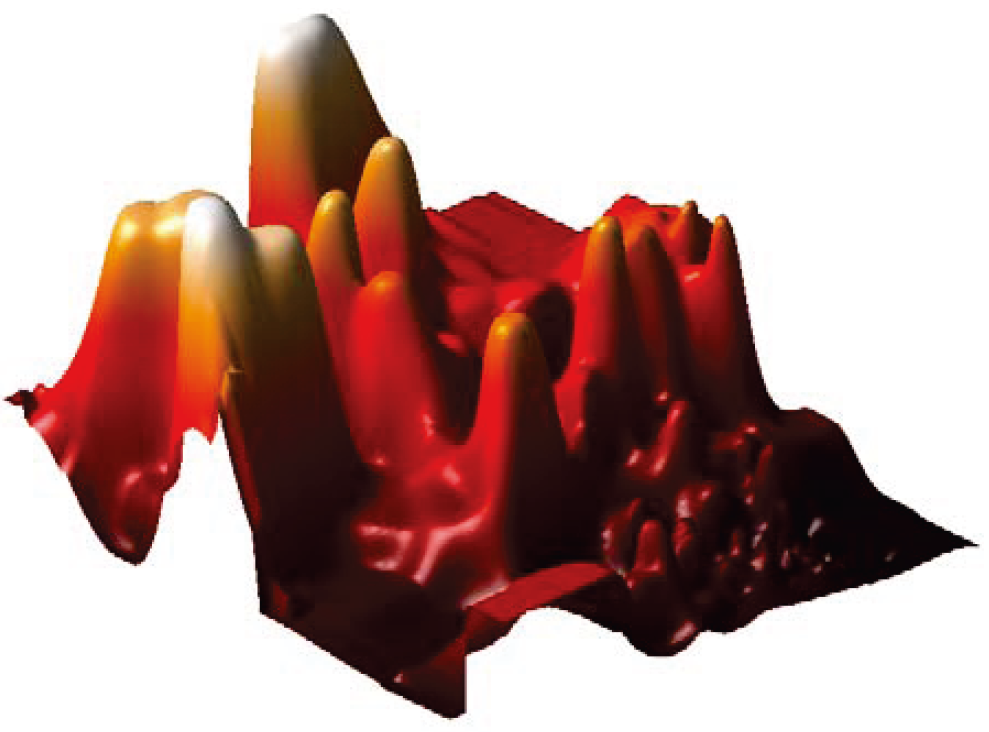
\includegraphics[scale=0.3]{pic/energy_landscape.png} \caption{\footnotesize
\textbf{2D projection of the reduced landscape of Au$_8$Pd$_4$, showing
clustering of low-energy structures in one region.} The landscape was produced
using the method of Oganov \& Valle (2009).}
\label{fig:energy_landscape}
\end{figure}

A major motivation for the development of USPEX was the discovery of the
post-perovskite phase of MgSiO$_3$ (Fig.~\ref{fig:structure_prediction_MgSiO3}),
which was made in 2004 \cite{Oganov2004, Murakami2004} and has significantly
changed models of the Earth's internal structure. In mid-2005 we had the first
working version of USPEX. By September 2010, when USPEX was publicly released,
the user community numbered nearly 200, over 800 users in May 2012, and over
2100 in December 2014.

\begin{figure}[htbp] \centering
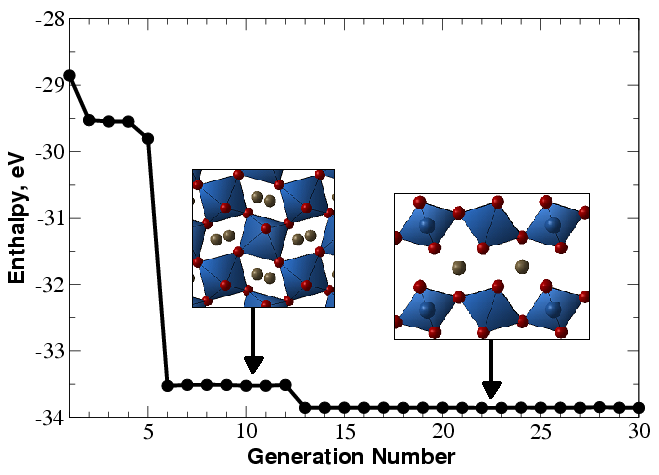
\includegraphics[scale=0.3]{pic/prediction_of_the_crystal_structure_of_MgSiO3.png}
\caption{\footnotesize \textbf{Prediction of the crystal structure of MgSiO$_3$
at 120~GPa (20~atoms/cell).} Enthalpy of the best structure as a function of
generation is shown. Between the 6$^{th}$ and 12$^{th}$ generations the best
structure is perovskite, but at the 13$^{th}$ generation the global minimum
(post-perovskite) is found. This simulation was performed in 2005 using one of
the first versions of USPEX combined with \emph{ab initio} calculations. It used
no experimental information and illustrates that USPEX can find both the stable
and low-energy metastable structures in a single simulation. Each generation
contains 30 structures. This figure illustrates the slowest of $\sim$10
calculations performed by the very first version of USPEX --- and even that was
pretty fast!}
\label{fig:structure_prediction_MgSiO3}
\end{figure}

The popularity of USPEX is due to its extremely high efficiency and reliability.
This was shown in the First Blind Test for Inorganic Crystal Structure
Prediction \cite{Oganov-book2010a}, where USPEX outperformed the other methods
it was tested against (simulated annealing and random sampling). Random sampling
(a technique pioneered for structure prediction by Freeman and Schmidt in 1993
and 1996, respectively, and since 2006 revived by Pickard \cite{Pickard2006}
under the name AIRSS) is the simplest, but also the least successful and
computationally the most expensive strategy. Even for small systems, such as
GaAs with 8 atoms/cell, these advantages are large (random sampling requires on
average 500 structure relaxations to find the ground state in this case, while
USPEX finds it after only $\sim$ 30 relaxations!
(Fig.~\ref{fig:structure_prediction_GaAs})). Due to the exponential scaling of
the complexity of structure search (eq.~\ref{eq:structNum}), the advantages of
USPEX increase exponentially with system size. For instance, 2 out of 3
structures of SiH$_4$ predicted by random sampling to be stable
\cite{Pickard2006}, turned out to be unstable \cite{Martinez-Canales2009}; and
similarly random sampling predictions were shown \cite{Ma2009} to be incorrect
for nitrogen \cite{Pickard2009a} and for SnH$_4$ (compare predictions
\cite{Gao2010} of USPEX and of random sampling \cite{Pickard2009b}).

\begin{figure}[hbtp] \centering
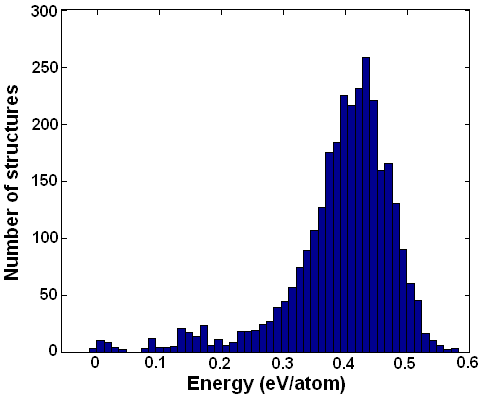
\includegraphics[scale=0.4]{pic/Structure_prediction_for_GaAs_a.png}
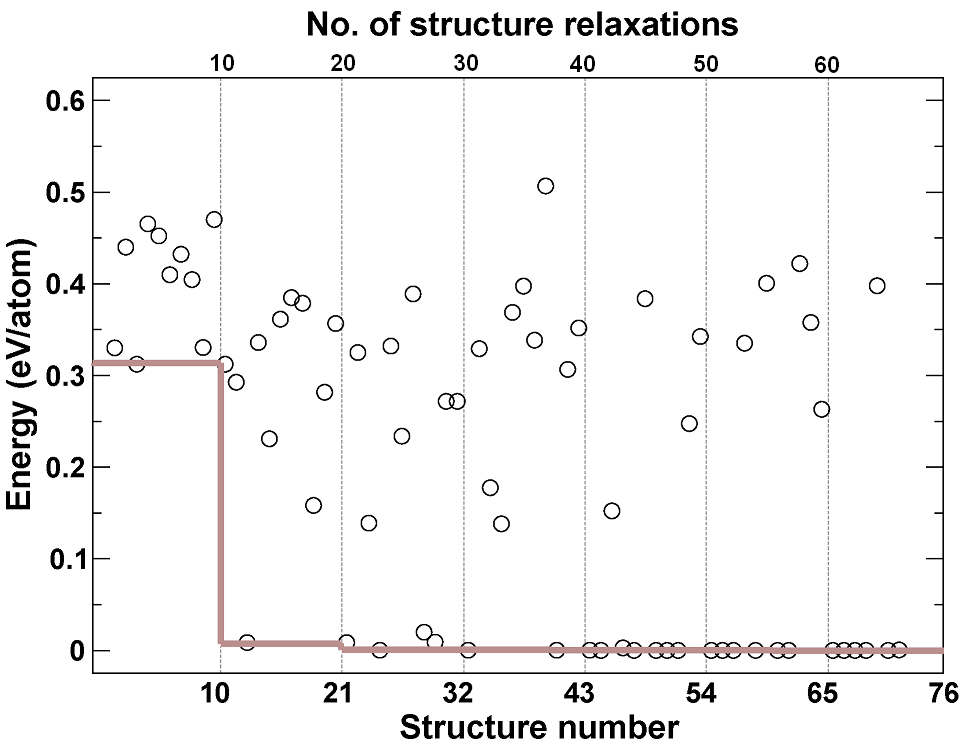
\includegraphics[scale=0.2]{pic/Structure_prediction_for_GaAs_b.png}
\caption{\footnotesize \textbf{Structure prediction for GaAs.} a) Energy
distribution for relaxed random structures, b) progress of an evolutionary
simulation (thin vertical lines show generations of structures, and the grey
line shows the lowest energy as a function of generation). All energies are
relative to the ground-state structure. The evolutionary simulation used 10
structures per generation. In addition, the lowest-energy structure of the
previous generation survived into the next generation.}
\label{fig:structure_prediction_GaAs}
\end{figure}

For larger systems, random sampling tends to produce almost exclusively
disordered structures with nearly identical energies, which decreases the
success rate to practically zero, as shown in the example of MgSiO$_3$
post-perovskite with 40 atoms/supercell --- random sampling fails to find the
correct structure even after 120,000 relaxations, whereas USPEX finds it
after several hundred relaxations (Fig.~\ref{fig:MgSiO3_40atoms}).

\begin{figure}[hbtp] \centering
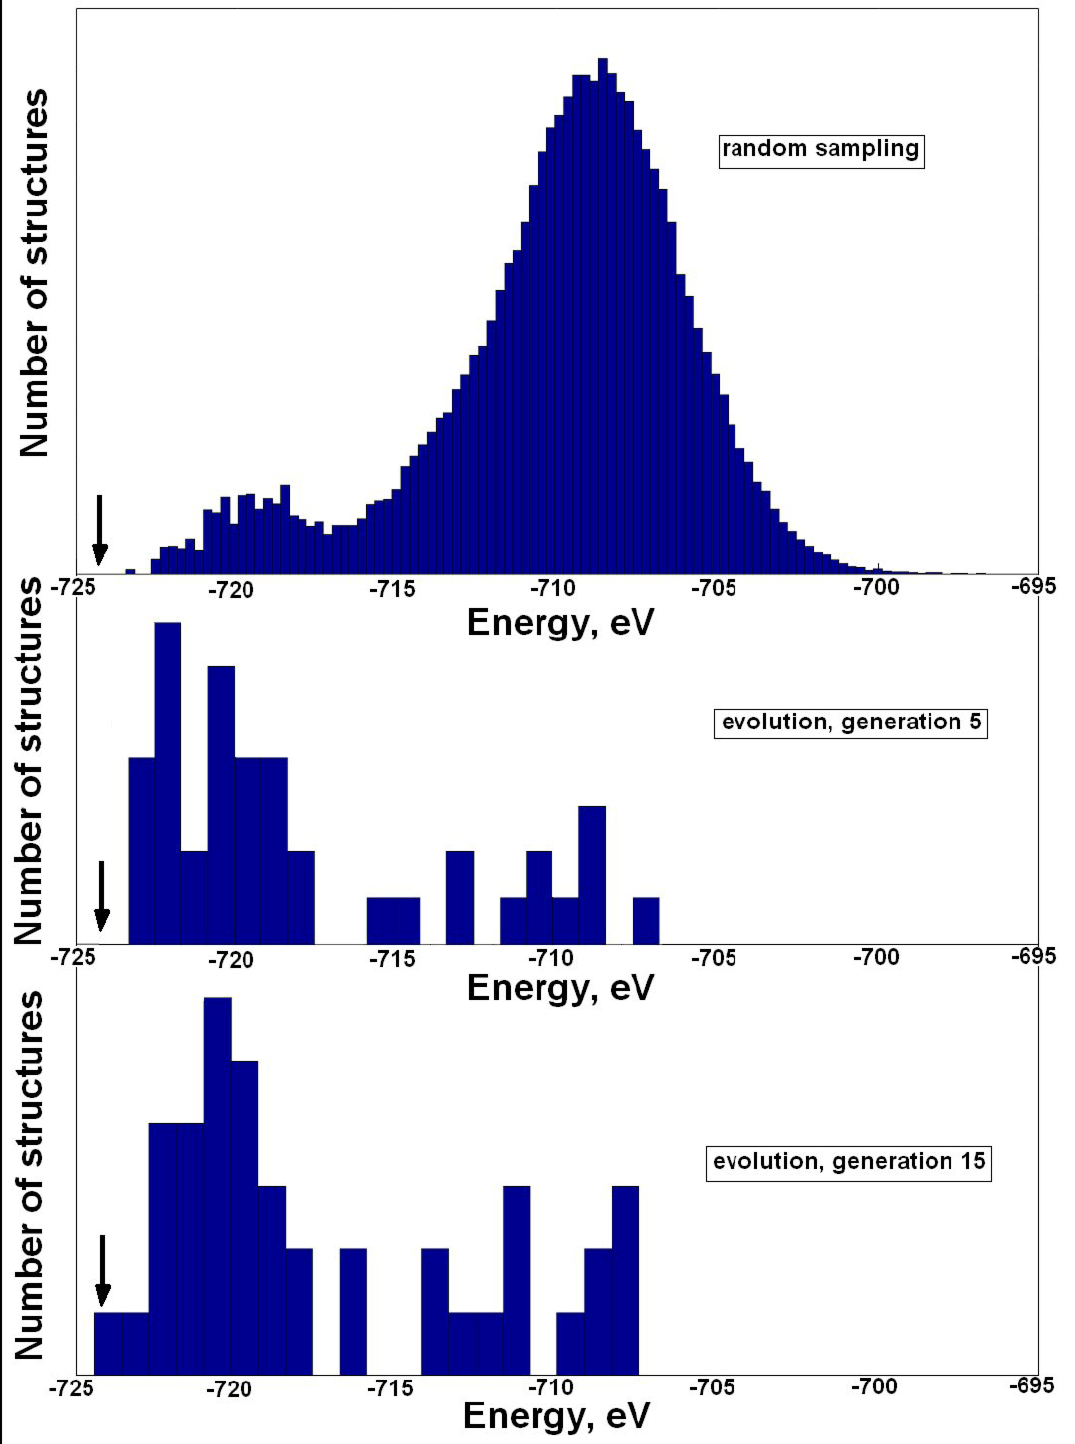
\includegraphics[scale=0.3]{pic/Sampling_of_the_energy_surface.png}
\caption{\footnotesize \textbf{Sampling of the energy surface: comparison of
random sampling and USPEX for a 40-atom cell of MgSiO$_3$ with cell parameters
of post-perovskite.} Energies of locally optimized structures are shown. For
random sampling, $1.2\times 10^{5}$ structures were generated (none of which
corresponded to the ground state). For USPEX search, each generation included 40
structures and the ground-state structure was found within 15 generations. The
energy of the ground-state structure is indicated by the arrow. This picture
shows that ``learning'' incorporated in evolutionary search drives the
simulation towards lower-energy structures.}
\label{fig:MgSiO3_40atoms}
\end{figure}

Random sampling runs can easily be performed with USPEX --- but we see this
useful mostly for testing. Likewise, the Particle Swarm Optimization (PSO)
algorithm for cluster and crystal structure prediction (developed by
A.I.~Boldyrev and re-implemented by Wang, Lu, Zhu and Ma) has been revamped and
implemented on the basis of USPEX with minor programming work as a corrected PSO
(corPSO) algorithm, which outperforms previous versions of PSO. Still, any
version of PSO is rather weak and we see the PSO approach suitable mostly for
testing purposes, if anyone wants to try. A very powerful new method,
complementary to our evolutionary algorithm, is evolutionary metadynamics
\cite{Lyakhov2013}, a hybrid of Marto\v{n}\'{a}k's metadynamics and the
Oganov-Glass evolutionary approach. This method is powerful for global
optimization and for harvesting low-energy metastable structures, and even for
finding possible phase transition pathways. For detailed investigations of phase
transition mechanisms, additional methods are implemented: variable-cell NEB
method \cite{Qian2013} and transition path method \cite{Dellago1998} in the
version \cite{Boulfelfel2012}.

\subsection{Features of USPEX}

\begin{itemize}

\item Prediction of the stable and metastable structures knowing only the
chemical composition. Simultaneous searches for stable compositions and
structures are also possible.

\item Incorporation of partial structural information is possible:
\begin{itemize}
  \item constraining search to fixed experimental cell parameters, or fixed cell
  shape, or fixed cell volume (Subsection~\ref{input_cell});
  \item starting structure search from known or hypothetical structures
  (Subsection~\ref{faq_seeds});
  \item assembling crystal structures from predefined molecules, including
  flexible molecules (Subsection~\ref{molecular_crystals}).
\end{itemize}

\item Efficient constraint techniques, which eliminate unphysical and redundant
regions of the search space. Cell reduction technique (Oganov \& Glass, 2008).

\item Niching using fingerprint functions (Oganov \& Valle, 2009; Lyakhov,
Oganov, Valle, 2010). Subsection~\ref{input_fingerprints} for details.

\item Initialization using fully random approach, or using space groups and cell
splitting techniques (Lyakhov, Oganov, Valle, 2010).

\item On-the-flight analysis of results --- determination of space groups (and
output in CIF-format) (Subsection~\ref{input_space_groups}), calculation of the
hardness, order parameters, \emph{etc}.

\item Prediction of the structure of nanoparticles and surface reconstructions.
See Section~\ref{surfaces} for details.

\item Restart facilities, enabling calculations to be continued from any point
along the evolutionary trajectory (Subsection~\ref{input_restart}).

\item Powerful visualization and analysis techniques implemented in the STM4
code (by M.~Valle), fully interfaced with USPEX
(Subsection~\ref{faq_visualization}).

\item USPEX is interfaced with VASP, SIESTA, GULP, LAMMPS, DMACRYS, CP2K,
Quantum Espresso, FHI-aims, ATK, CASTEP, Tinker, MOPAC codes. See full list of
supported codes in Subsection~\ref{abinitio_codes}. Interfacing with other codes
is easy.

\item Submission of jobs from local workstation to remote clusters and
supercomputers is possible. See Section~\ref{faq_job_submit} for details.

\item Options for structure prediction using the USPEX algorithm (default),
random sampling, corrected particle swarm optimization (Subsection~\ref{pso}),
evolutionary metadynamics (Subsection~\ref{metadynamics}), minima hopping-like
algorithm. Capabilities to predict phase transition mechanisms using
evolutionary metadynamics, variable-cell NEB method (Subsection~\ref{vcneb}),
and TSP method (Subsection~\ref{tps}).

\item Options to optimize physical properties other than the energy ---
\emph{e.g.}, hardness (Lyakhov \& Oganov, 2011), density (Zhu et al., 2011),
band gap and dielectric constant (Zeng et al., 2014), and many other properties.

\item For ease of programming and use, USPEX is written in MATLAB and it also
works under Octave (a free MATLAB-like environment) --- you do not need to
compile anything, just plug and play! To enhance MATLAB-version compatibility,
only basic MATLAB commands have been used. The code has been developed and
tested under Matlab 2012 to 2015 and Octave~3.4 (\emph{newer Octave versions are
not supported yet!}).

\item Starting from version 9.4.1, USPEX has an installer (\file{install.sh}
file) and a Python-based runner of MATLAB code (\file{USPEX} Python module),
providing a number of useful command line options.

\end{itemize}

\subsection{Key USPEX method and application papers}

\begin{enumerate}

\item Oganov A.R., Glass C.W. (2006). Crystal structure prediction using
evolutionary algorithms: principles and applications. \emph{J. Chem. Phys.},
\textbf{124}, 244704.

\item Oganov A.R., Stokes H., Valle M. (2011). How evolutionary crystal
structure prediction works --- and why. \emph{Acc. Chem. Res.}, \textbf{44},
227--237.

\item Lyakhov A.O., Oganov A.R., Stokes H., Zhu Q. (2013). New developments in
evolutionary structure prediction algorithm USPEX. \emph{Comp. Phys. Comm.},
\textbf{184}, 1172--1182.

\item Zhu Q., Oganov A.R., Glass C.W., Stokes H. (2012). Constrained
evolutionary algorithm for structure prediction of molecular crystals:
methodology and applications. \emph{Acta Cryst. B}, \textbf{68}, 215--226.

\item Zhu Q., Li L., Oganov A.R., Allen P.B. (2013). Evolutionary method for
predicting surface reconstructions with variable stoichiometry. \emph{Phys. Rev.
B}, \textbf{87}, 195317.

\item Zhu, Q., Sharma V., Oganov A.R., Ramprasad R. (2014). Predicting polymeric
crystal structures by evolutionary algorithms. \emph{J. Chem. Phys.},
\textbf{141}, 154102.

\item Zhou X.-F., Dong X., Oganov A.R., Zhu Q., Tian Y., Wang H.-T. (2014).
Semimetallic Two-Dimensional Boron Allotrope with Massless Dirac Fermions.
\emph{Phys. Rev. Lett.}, \textbf{112}, 085502.

\item Lyakhov A.O., Oganov A.R., Valle M. (2010). Crystal structure prediction
using evolutionary approach. In: Modern methods of crystal structure prediction
(ed: A.R. Oganov), Berlin: Wiley-VCH.

\item Oganov A.R., Ma Y., Lyakhov A.O., Valle M., Gatti C. (2010). Evolutionary
crystal structure prediction as a method for the discovery of minerals and
materials. \emph{Rev. Mineral. Geochem.}, \textbf{71}, 271--298.

\item Duan, D., Liu, Y., Tian, F., Li, D., Huang, X., Zhao, Z., Yu, H., Liu, B.,
Tian, W., Cui, T. (2014). Pressure-induced metallization of dense
(H$_2$S)$_2$H$_2$ with high-$T_c$ superconductivity. \emph{Sci. Rep.},
\textbf{4}.
 
\end{enumerate}


%%%%%%%%%%%%%%%%%%%%%%%%%%%%%%%%%%%%%%%%%%%%%%%%%%%%%%%%%%%%%%%%%%%%%%%%%%%%%%%%

\subsection{Version history (only important versions listed)}

{\small
\textbf{v.1} --- Evolutionary algorithm without local optimization. Real-space
representation, interface with VASP. Experimental version. October 2004.

\textbf{v.2} --- CMA-ES implementation (CMA-ES is a powerful global optimization
method developed by N.~Hansen). Experimental version. January 2005.

\textbf{v.3} --- Evolutionary algorithm with local optimization.

\textbf{v.3.1} --- Working versions, sequential. Major basic developments. 

3.1.4-3.1.5 --- First production version. Based largely on heredity with
slice-shifting and with minimum-parent contribution (hard-coded to be 0.25). May
2005.

3.1.8 --- Adaptive $k$-point grids. 15/10/2005. 

3.1.11 --- Restart from arbitrary generation. Experimental version. 04/11/2005. 

3.1.12 --- Production version based on v.3.1.11, variable slice-shift mutation.
11/11/2005.

3.1.13 --- Adaptive scaling volume. 29/11/2005.

3.1.14 --- Basic seed technique. 29/11/2005 (debugged 6/12/2005). 

\textbf{v.3.2} --- Massively parallel version. 

\textbf{v.4} --- Unified parallel/sequential version. 

4.1.1 --- Lattice mutation. 20/12/2005 (debugged 10/01/2006).

4.2.1 --- Interfaced with SIESTA. Initial population size allowed to differ from
the running population size. 24/01/2006 (debugged 20/04/2006).

4.2.3 --- Relaxation of best structures made optional. Version with fully
debugged massive parallelism. 25/04/2006.

4.4.1 --- Interfaced with GULP. 08/05/2006.

\textbf{v.5} --- Completely rewritten and debugged version, clear modular
structure of the code.

5.1.1 --- Atom-specific permutation, code interoperability, on-the-fly reading
of parameters from \file{INPUT\_EA.txt}. 20/12/2006.

5.2.1 --- SIESTA-interface for Z-matrix, rotational mutation operator.
01/03/2007.

\textbf{v.6} --- Production version.

6.1.3 --- To efficiently fulfill hard constraints for large systems, an
optimizer was implemented within USPEX. 07/06/2007.

6.2 --- Development version.

6.3.1--6.3.2 --- Introduced angular constraints for cell diagonals. Completely
rewritten remote submission. Improved input format. Further extended standard
tests. 07/12/2007.

6.3.3 --- X-com grid interface (with participation of S.~Tikhonov and
S.~Sobolev). 05/03/2008.

6.4.1 --- Fingerprint functions for niching. 07/04/2008.

6.4.4 --- Space group recognition. Fast fingerprints (from tables). 05/05/2008.

6.5.1 --- Split-cell method for large systems. Easy remote submission.
Variable number of best structures (clustering). 16/07/2008.

6.6.1 --- A very robust version --- improved fingerprint and split-cell
implementations. 13/08/2008.

6.6.3 --- Heredity with multiple parents implemented. 01/10/2008.

6.6.4 --- Added a threshold for parents participating in heredity (niching).
03/10/2008.

6.6.6 --- First implementation of multicomponent fingerprints. 04/12/2008.

6.6.7, 6.7.1 and 6.7.2 --- Implemented quasi-entropy to measure the diversity of
the population. 10/12/2008.

\textbf{v.7} --- Production version, written to include variable composition. 

7.1.1--7.1.7 --- Series of improved versions. Version 7.1.7 has been distributed
to $\sim$200 users. Variable composition partly coded, most known bugs fixed,
improved tricks based on energy landscapes. Improved cell splitting, implemented
pseudo-subcells. Implemented multicomponent fingerprints (much more sensitive to
the structure than one-component fingerprints). 28/04/2009 (version finalized
28/05/2009).

7.2.5 --- First fully functional version of the variable-composition method.
Introduced transmutation operator and compositional entropy. 06/09/2009.

7.2.7 --- Thoroughly debugged, improved restart capabilities, improved seeding,
introduced perturbations within structure relaxation. 25/09/2009, further
improved in versions 7.2.8/9.

7.3.0 --- Full fingerprint support in the variable-composition code, including
niching. ``Fair'' algorithm for producing the first generation of compositions.
22/10/2009.

7.4.1 --- Introduced coordinate mutation based on local order \cite{Oganov2009}.
Heredity and transmutation are also biased by local order. Introduced
computation of the hardness and new types of optimization by hardness and
density. 04/01/2010.

7.4.2 --- Implementation of multiple-parents heredity biased by local order.
15/01/2010.

7.4.3 --- Implementation of new types of optimization (to maximize
structural order and diversity of the population). Implemented antiseeds,
eliminated parameters \keyword{volTimeConst}, \keyword{volBestHowMany}.
24/01/2010.

\textbf{v.8} --- Production version, written to include new types of
optimization.

8.1.1--8.2.8 --- Development versions. Local order and coordinate mutation
operator. Softmutation operator. Calculation and optimization of the hardness.
Optimization of the dielectric susceptibility. Prediction of the structure of
nanoparticles and surfaces. Implementation of point groups. Greatly improved
overall performance. Option to perform PSO simulations (not recommended for
applications, due to PSO's inferior efficiency --- so use only for testing
purposes). Parameter \keyword{goodBonds} transformed into a matrix and used for
building nanoparticles. 22/09/2010.

8.3.1 --- Optimization of dielectric constants, cleaned-up input. 08/10/2010.

8.3.2 --- For clusters, introduced a check on connectivity (extremely useful),
\keyword{dynamicalBestHM}=2 option improved, as well as mechanism for producing
purely softmutated generations. Improved fingerprints for clusters.
Interface to Quantum Espresso and CP2K codes. 11/10/2010.

8.4 --- Improved antiseed functionalities and several improvements for
nanoparticles. Development branches for surface reconstructions,
pseudo-metadynamics, molecular crystals.

8.5.0 --- Initialization of the first random generation using the space group
code of H.~Stokes added. New formulation of metadynamics implemented and
finalized, for now in a separate code. Several debugs for varcomp, antiseeds,
nanoparticles, computation of hardness. 18/03/2011.

8.5.1 --- Space group initialization implemented for cases of fixed unit cell,
variable composition, and subcells. 20/04/2011.

8.6.0 --- Added space group determination program from H.~Stokes. Merger with
the updated code for molecular crystals (including space group initialization).
Fixed a bug for SIESTA (thanks to D.~Skachkov). 06/05/2011.

8.6.1--8.7.2 --- Improved symmetric initialization for the case of a fixed cell.
Implemented optimization of dielectric constants (using GULP and VASP), band gap
(using VASP), and DOS at the Fermi level (VASP). Graphical output enabled.
Improved softmutation (by using better criteria for mode and directional
degeneracies) and heredity (by using energy-order correlation coefficient and
cosine formula for the number of trial slabs) operators. Most variables now have
default values, which enables the use of very short input files. Shortened and
improved the format of log-files. 13/11/2011.

8.7.5 --- Graphical output now includes many extra figures. Added utility to
extract all structures close to convex hull for easier post-processing.
21/03/2012.

\textbf{v.9} --- Production version, made more user-friendly and written to
include new types of functionality and to set the new standard in the field.

9.0.0 --- Evolutionary metadynamics and vc-NEB codes added to USPEX package,
added tensor version of metadynamics, added additional figures and
post-processing tools, cleaned the code output. A few parameters removed from
the input. Improved softmutation. April 2012.

9.1.0 --- Release version. Cleaned up, documented. The user community is $>$800
people. Released 28/05/2012.

9.2.0 --- Working GEM. Constant development of the GEM code. Space group
determination tolerance is now an input parameter. Improved default for number
of permutations. July-August 2012.

9.2.1--9.2.3 --- Improved GEM, more diverse populations and supercell sizes,
improved mode selection. September-October 2012.

9.2.4--9.2.6 --- (9.2.4 is a release version). Intelligent defaults for most
input parameters. Improved symmetric initialization for clusters. Order-enhanced
heredity for nanoparticles. New parameter to tune the tolerance for the space
group determination. New property (quasientropy) can be optimized. Fully
integrated vc-NEB code. November-December 2012.

9.2.7. --- Release version. Enabled optimization of order for alloys, without
structure relaxation (for easy creation of quasirandom structures, based on the
more general definition than the so-called ``special quasi-random structures'').
Symmetry generation was improved (particularly important for fixed-cell
calculations). For fixed-cell calculations, one can now specify the cell
parameters, not only in the form of a 3 $\times$ 3 matrix, but also as a row of
six values (three lengths in Angstroms and three angles in degrees). For the
maximum number of permutation swaps (parameter \keyword{howManySwaps}), we have
introduced an intelligent default. Added new tests, and cleaned and reran the
old ones. Added interface to CASTEP (thanks to Z.~Raza, X.~Dong and AL). User
community 1160 people. 30/12/2012.

9.3.0--9.3.3 --- Fixed a bug in generation of random symmetric structures (this
bug appeared in 9.2.7). Significantly simplified input and output. Created file
\file{OUTPUT.txt} with the most important information. Enabled split-cell trick
for molecular crystals. Improved variable-composition calculations by allowing
one to specify initial compositions. Added interface to CASTEP and LAMMPS. Added
new test cases. 20/03/2013.

9.3.4 --- Release version, cleaned up. 25/03/2013. 

9.3.5 --- Added code for prediction of 2D-crystals. 19/04/2013.

9.3.6 --- Incorporated plane groups for 2D-crystals. 29/04/2013.

9.3.8 --- Incorporated plane groups for 1D-polymer crystals, improved variables
of stoichiometry for surfaces. 19/06/2013.

9.3.9 --- Released version. Significantly improved version, improved
user-friendliness, new functionalities (2D-crystals, GEM) made more robust,
improvements in the variable-composition algorithm (and enabled support for
single-block calculations, \emph{i.e.} fixed-composition searches with variable
number of atoms in the cell), fully functional surface calculations, new
optimization types (can optimize band gaps, dielectric constants, and newly
invented figure of merit of dielectric materials). Interfaces with LAMMPS and
ATK are documented in new test cases. Continuously updated with minor debugs
(last debug 10/02/2014). 19/07/2013.

9.4.1 --- A major upgrade, greatly improved user-friendliness (automatic
estimate of volumes and of percentages of variation operators for each case),
new functionalities (optimization of elastic properties and Chen's model of
hardness, prediction of polymeric structures, anti-compositions, automatic
analysis of statistics, improved seed technique), first release of GEM
(generalized evolutionary metadynamics), provided a set of real-life examples of
USPEX calculations, test cases, documentation.
More than 2100 users. Released 30/12/2014.

9.4.2 --- Release version, compatible with Octave 3.4. Convex hull code
rewritten. Interface with MOPAC implemented. Default values for
\keyword{goodBonds}, \keyword{valences}, \keyword{IonDistances} enabled.
More robust for ternary, quaternary, and more complex variable-composition
searches. Robust TPS implementation (only for developers, will be available for
users soon). More than 2200 users. Released 21/03/2015.

9.4.3 --- Release version. It includes fixing a number of bugs (which should
slightly speed up performance), interface with MOPAC, improved documentation.
Released 10/08/2015.

9.4.4 --- Release version. It includes fix for space group determination and
other problems reported by users, improved documentation and examples, full
Octave 3.4 compatibility and partial Octave 3.6/3.8/4.0 support. This version
should be nearly bug-free and is a milestone towards a very major upgrade, which
will be made available in version 10. Released 05/10/2015.
}

%%%%%%%%%%%%%%%%%%%%%%%%%%%%%%%%%%%%%%%%%%%%%%%%%%%%%%%%%%%%%%%%%%%%%%%%%%%%%%%%
\newpage
\section{Getting started}

\subsection{How to obtain USPEX}

USPEX is an open source code, and can be downloaded at:
\begin{center}
\textcolor{blue}{\url{http://uspex.stonybrook.edu}}
\end{center}

In the download page, there are separate packages for USPEX source code, example
and manual files.

\subsection{Necessary citations}
Whenever using USPEX, in all publications and reports you must cite the original
papers, for example, in the following way:

\begin{quote}
``Crystal structure prediction was performed using the USPEX code
\cite{Oganov2006, Oganov2011, Lyakhov2013}, based on an evolutionary algorithm
developed by Oganov, Glass, Lyakhov and Zhu and featuring local optimization,
real-space representation and flexible physically motivated variation
operators''.
\end{quote}

Consult the \file{OUTPUT.txt} file for some of the most important references.

\subsection{Bug reports}

Like any large code, USPEX may have bugs. If you see strange behavior in your
simulations, please report it to us in USPEX Google group at:

\begin{center}
\textcolor{blue}{\url{https://groups.google.com/forum/#!forum/uspex}}
\end{center}

Please describe your problem in details and attach \file{INPUT.txt},
\file{OUTPUT.txt}, \file{log} and other related files when you report a problem.
You can also send the questions or problem descriptions to USPEX master
(currently --- Qiang Zhu
(\href{mailto:alecfans@gmail.com}{alecfans@gmail.com})).

\subsection{On which machines can USPEX be run}
USPEX can be used on any unix-based platform --- all you need is one CPU where
MATLAB or Octave can be run under Linux or Unix --- using its special remote
submission mechanism, USPEX will be able to connect to any remote machine
(regardless of whether MATLAB is installed there) and use it for calculations.

\subsection{Codes that can work with USPEX} \label{abinitio_codes}

Trial structures generated by USPEX are relaxed and then evaluated by an
external code interfaced with USPEX. Based on the obtained ranking of relaxed
structures, USPEX generates new structures --- which are again relaxed and
ranked. Our philosophy is to use existing well-established \emph{ab initio} (or
classical forcefield) codes for structure relaxation and energy calculations.
Currently, USPEX is interfaced with:

\begin{itemize}
\item VASP --- \url{https://www.vasp.at/}
\item SIESTA --- \url{http://departments.icmab.es/leem/siesta/}
\item GULP --- \url{http://nanochemistry.curtin.edu.au/gulp/}
\item LAMMPS --- \url{http://lammps.sandia.gov/}
\item DMACRYS --- \url{http://www.chem.ucl.ac.uk/basictechorg/dmacrys/index.html}
\item CP2K --- \url{http://www.cp2k.org/}
\item Quantum Espresso --- \url{http://www.quantum-espresso.org/}
\item FHI-aims --- \url{https://aimsclub.fhi-berlin.mpg.de/}
\item ATK --- \url{http://quantumwise.com/}
\item CASTEP --- \url{http://www.castep.org/}
\item Tinker --- \url{http://dasher.wustl.edu/tinker/}
\item MOPAC --- \url{http://openmopac.net/}
\end{itemize}

The choice of these codes was based on 1) their efficiency for structure
relaxation; 2) robustness; and 3) popularity. Of course, there are other codes
that can satisfy these criteria, and in the future we can interface USPEX to
them.

\subsection{How to install USPEX}
After you download the archive with USPEX, you need to unpack it and run the
following command to install USPEX to a user's or system-wide location:
\begin{verbatim}
    bash ./install.sh
\end{verbatim}

The installer does not require root privileges. You will be asked to select
MATLAB or Octave (if it is found in the system), installation directory and to
confirm creation/using of that directory. Then you will be provided with
information about environmental variables, which must be set to make USPEX
available in the system. For example:

{\footnotesize
\begin{verbatim}
   For Bash shell system, add these lines in ~/.bashrc or ~/.profile or /etc/profile:
     export PATH=/home/user/bin/USPEX:$PATH
     export USPEXPATH=/home/user/bin/USPEX/src

   For C shell system, add these lines in ~/.cshrc or ~/.profile or /etc/profile:
     setenv PATH "/home/user/bin/USPEX:$PATH"
     setenv USPEXPATH "/home/user/bin/USPEX/src"
\end{verbatim}
}

If you want to change the path of MATLAB or Octave, you can edit the file
\file{CODEPATH} in the installation directory of USPEX.

\subsection{How to run USPEX}
To run USPEX, you need to have MATLAB (preferred) or Octave and to have the
executable of the external code on the compute nodes that you use for relaxing
structures and computing their energies (see Subsection~\ref{abinitio_codes} for
a list of supported codes). To set up your calculation, find an example (see
Appendix~\ref{appendix_examples} for a list of examples), similar to what you
want to do, and start by editing \file{INPUT.txt}. The variables of this crucial
file are described in Section~\ref{inputs} below. Then, gather the files needed
for the external code performing structure relaxation in the \file{Specific/}
folder --- the executable (\emph{e.g.}, \file{vasp}), and such files as
\file{INCAR\_1}, \file{INCAR\_2}, \ldots, \file{INCAR\_\emph{N}}, and
\file{POTCAR\_\emph{A}}, \file{POTCAR\_\emph{B}}, \ldots, where
\texttt{\emph{A}}, \texttt{\emph{B}}, \ldots are the short symbols of the
chemical elements described in the corresponding \file{POTCAR} files.

There are two ways to run the code --- old and new, and both work.

(i) In the old way, you need to have the entire USPEX code (file \file{USPEX.m},
directory \file{FunctionFolder}, etc.) in your execution folder. Then type
\begin{verbatim}
    nohup matlab < USPEX.m > log &
\end{verbatim}

or, if you use Octave, type
\begin{verbatim}
    nohup octave < USPEX.m > log &
\end{verbatim}

(ii) In the new way, if you used the USPEX installer for the Python-based
runner, all you need to execute the code is just type:
\begin{verbatim}
    nohup USPEX -r > log &
\end{verbatim}

or, if you use Octave, type
\begin{verbatim}
    nohup USPEX -r -o > log &
\end{verbatim}

File \file{log} will contain information on the progress of the simulation and,
if any, errors (send these to us, if you would like to report a bug).

File \file{OUTPUT.txt} will contain details of the calculation and an analysis
of each generation.

\vspace{\baselineskip}
For the USPEX runner, we have a number of user-friendly options:
\begin{itemize}
   \item[] \textbf{-v, -{}-version}:  show program's version number and exit
   \item[] \textbf{-h, -{}-help}:   show this help message and exit
   \item[] \textbf{-p, -{}-parameter}: specify parameter to get help. If no value or 'all' value is specified, all INPUT.txt parameters will be shown
   \item[] \textbf{-e, -{}-example}: show USPEX example details. If no value or 'all' value is specified, all examples will be shown
   \item[] \textbf{-c NUM, -{}-copy=NUM}: copy the INPUT.txt file and Specific Folder of ExampleXX.
   \item[] \textbf{-g, -{}-generate}:  generate directories for preparing an USPEX calculation, including AntiSeeds, Seeds, Specific, Submission folders
   \item[] \textbf{-r, -{}-run}:    run USPEX calculation
   \item[] \textbf{-o, -{}-octave}:    run USPEX calculation with Octave instead of MATLAB
   \item[] \textbf{-{}-clean}:    clean calculation folder
\end{itemize}

When running USPEX in the massively parallel mode, the user needs to do minimal
work to configure files to the user's computers (hence, we cannot guarantee
support for solving problems with massively parallel mode).

There are two modes for job submission --- (1) local submission and (2) remote
submission, depending on whether you submit \emph{ab initio} calculations on the
same machine where you run USPEX and MATLAB, or if you send your jobs to a
remote supercomputer. See the keyword \keyword{whichCluster} and
Subsection~\ref{faq_job_submit} of this Manual.

Please note, that you shoud have \file{bash} shell set by default to make USPEX
working correctly. Users frequently report issues when running USPEX on a
machine with \file{csh} shell, where ``\texttt{echo -e \ldots}'' command might
not be supported.

\subsection{Running USPEX examples: a mini-tutorial}
Once you have downloaded the USPEX package and installed it, you can run the
first USPEX example. The description of the examples is listed in
Appendix~\ref{appendix_examples}. The required external codes to run the
examples (except EX13) are shown below:

{\small\begin{itemize}
\item GULP: EX02, EX03, EX08, EX12, EX15 (VC-NEB), EX16
\item VASP: EX01, EX07, EX09, EX14 (META)
\item LAMMPS: EX04
\item ATK: EX05
\item CASTEP: EX06
\item DMACRYS: EX10
\item Tinker: EX11
\end{itemize}}

Now, let us start our first USPEX experience:

\subsubsection{Test the USPEX python runner}
To get the version information, you can use the following command:

\texttt{>> USPEX -v}

You should get the following information:
{\small\begin{verbatim}
  USPEX Version 9.4.2 (19/03/2015)
\end{verbatim}
}
If it does not work, please check your installation procedure and environment
settings as described above.

\subsubsection{Run the EX13-3D\_special\_quasirandom\_structure\_TiCoO} 
EX13 does not require any external code, you can run it to get familiar with the
USPEX running procedure. The calculation would take $\sim$30 minutes. To start
the calculation, first create a test folder, copy the example files and then run
the calculation through the USPEX Python runner, with the following commands:

\texttt{>> mkdir EX13}\\
\texttt{>> cd EX13}\\
\texttt{>> USPEX -c 13}\\
\texttt{>> USPEX -r}\\

Meanwhile you have some time to get more details about example EX13. In EX13,
the structural order is optimized (minimized) with the evolutionary algorithm.
Therefore in \file{INPUT.txt} the following is set:

{\small\begin{verbatim}
USPEX : calculationMethod
-4    : optType
\end{verbatim}}

and these parameters are used below:
{\small\begin{verbatim}
300   : calculationType

% atomType
Co Ti O
% EndAtomType

% numSpecies
16 16 64
% EndNumSpecies
\end{verbatim}}

to specify USPEX to evaluate the Co$_{16}$Ti$_{16}$O$_{64}$ system. To reduce
calculation time of EX13, you can reduce \keyword{populationSize} and
\keyword{numGenerations}, for example:
{\small\begin{verbatim}
5    : populationSize
5    : numGenerations
\end{verbatim}}

However, with such a small \keyword{populationSize} and
\keyword{numGenerations}, you cannot expect USPEX to find the structure with the
lowest order. Since you do not need to use any external code, you can simply set
{\small\begin{verbatim}
% abinitioCode
0
% ENDabinit
\end{verbatim}}

The \file{Seeds/POSCARS} file contains the initial Ti$_{16}$Co$_{16}$O$_{64}$
structure.

When you find the \file{USPEX\_IS\_DONE} file, congratulations, you have
successfully finished your first USPEX example. Next, you can run calculations
using external codes.

\subsubsection{Run an example using external code}
In this step, we suggest to run examples interfaced with GULP or VASP, starting
from EX02 or EX01. You will also use USPEX runner to get the example information
of EX02, create a separate folder and copy the files, with commands:
 
\texttt{>> mkdir EX02}\\
\texttt{>> cd EX02}\\
\texttt{>> USPEX -c 2}\\

Since in example EX02 GULP code is used, set: 
{\small\begin{verbatim}
% abinitioCode
3 3 3 3
% ENDabinit
\end{verbatim} }

To run a serial job without a job batch system, you should change the following
parameters in the \file{INPUT.txt} below:
{\small\begin{verbatim}
0     : whichCluster 
1     : numParallelCalcs
\end{verbatim} }

In the example \file{INPUT.txt} file \keyword{whichCluster}=QSH, where QSH is
our group's cluster name. We also provide the same way to help users to define
their own cluster. For more details, please see Section~\ref{faq_job_submit}.

In \file{INPUT.txt}, we do not specify how to run GULP, because we assume all
users use the same command:

{\small \begin{verbatim}
% commandExecutable
gulp < input > output
% EndExecutable
\end{verbatim} }

But make sure, this command also works on your machine. If you want to run EX01
with a parallel version of VASP, you should set something like:

{\small\begin{verbatim}
% abinitioCode
1 1 1 1
% ENDabinit

% commandExecutable
mpirun -np 8 vasp
% EndExecutable
\end{verbatim}}

With wrong \keyword{commandExecutable} settings, you will fail to start the
USPEX calculation. When everything is set correctly, we can run the calculation
through USPEX runner using the command:
 
\texttt{>> USPEX -r}


\subsubsection{Checking the results}
After starting the command, you can check the output files in \file{results1/}
folder.

Now, you have a basic experience of using USPEX to run simple calculations.
Please read the following sections of this manual to get more insight into
USPEX.

%%%%%%%%%%%%%%%%%%%%%%%%%%%%%%%%%%%%%%%%%%%%%%%%%%%%%%%%%%%%%%%%%%%%%%%%%%%%%%%% 

\newpage
\section{Overview of input and output files}

Input/output files depend on the external code used for structure relaxation.

An important technical element of our philosophy is the multi-stage strategy for
structure relaxation. Final structures and energies must be high-quality, in
order to correctly drive evolution. Most of the newly generated structures are
far from local minimum and their high-quality relaxation is extremely expensive.
This cost can be avoided if the first stages of relaxation are done with cruder
computational conditions --- only at the last stages of structure relaxation is
there a need for high-quality calculations. The first stages of structure
relaxation can be performed with cheaper approaches. You can change the
computational conditions (basis set, $k$-points sampling, pseudopotentials or
PAW potentials) or the level of approximation (interatomic potentials \emph{vs.}
LDA \emph{vs.} GGA) or even the structure relaxation code (see
Subsection~\ref{abinitio_codes} for a list of supported codes) during structure
relaxation of each candidate structure. We strongly suggest that you initially
optimize the cell shape and atomic positions at constant unit cell volume, and
only then perform full optimization of all structural variables. While
optimizing at constant volume, you do not need to worry about Pulay stresses in
plane-wave calculations --- thus it is OK to use a small basis set; however, for
variable-cell relaxation you will need a high-quality basis set. For structure
relaxation, you can often get away with a small set of $k$-points --- but don't
forget to sufficiently increase this at the last stage(s) of structure
relaxation, to get accurate energies.

\subsection{Input files}

Suppose that the directory where the calculations are performed is
\file{$\sim$/StructurePrediction}. This directory will contain:

\begin{itemize}

\item file \file{INPUT.txt}, thoroughly described in Section~\ref{inputs}.

\item Subdirectory \file{$\sim$/StructurePrediction/Specific/} with VASP,
SIESTA or GULP (\emph{etc.}) executables, and enumerated input files for
structure relaxation --- \file{INCAR\_1}, \file{INCAR\_2}, \ldots, and
pseudopotentials.

\item Subdirectory \file{$\sim$/StructurePrediction/Seeds} --- contains files
with seed structures and with a list of compositions/anti-compositions. Seed
structures should be in VASP5 POSCAR format and concatenated in a file called
\file{POSCARS} or \file{POSCARS\_gen} (\texttt{gen} is the generation number).
The \file{compositions} and \file{Anti-compositions} files are used to control
the compositions during variable-composition or single-block calculations.

\item Subdirectory \file{$\sim$/StructurePrediction/AntiSeeds} --- you may put
here particular structures that you wish to penalize, or use antiseed technique
without specifying any structures explicitly (and penalize structures found
during the run).

\end{itemize}

\subsection{Output files}
There usually is a result folder  \file{$\sim$/StructurePrediction/results1} for
storing the results of a USPEX calculation. If this is a new calculation,
\file{results2}, \file{results3}, \ldots (if the calculation has been restarted
or run a few times), there will be a separate \file{results*} folder for each
calculation.

The subdirectory \file{$\sim$/StructurePrediction/results1} contains the
following files:

\begin{itemize}

\item \file{OUTPUT.txt} --- summarizes input variables, structures produced by
USPEX, and their characteristics.

\item \file{Parameters.txt} --- this is a copy of the \file{INPUT.txt} file
used in this calculation, for your reference.

\item \file{Individuals} --- gives details of all produced structures
(energies, unit cell volumes, space groups, variation operators that were used
to produce the structures, $k$-points mesh used to compute the structures' final
energy, degrees of order, \emph{etc.}). File \file{BESTIndividuals} gives this
information for the best structures from each generation. Example of
\file{Individuals} file:

{\tiny
\begin{verbatim}
Gen   ID    Origin   Composition    Enthalpy   Volume  Density   Fitness   KPOINTS  SYMM  Q_entr A_order S_order
                                      (eV)      (A^3)  (g/cm^3)
  1    1   Random    [   4  8 16 ]  -655.062   201.062   4.700   -655.062 [ 1  1  1]   1   0.140  1.209  2.632
  1    2   Random    [   4  8 16 ]  -650.378   206.675   4.572   -650.378 [ 1  1  1]   1   0.195  1.050  2.142
  1    3   Random    [   4  8 16 ]  -646.184   203.354   4.647   -646.184 [ 1  1  1]   1   0.229  0.922  1.746
  1    4   Random    [   4  8 16 ]  -649.459   198.097   4.770   -649.459 [ 1  1  1]   9   0.128  0.958  2.171
  1    5   Random    [   4  8 16 ]  -648.352   202.711   4.662   -648.352 [ 1  1  1]   2   0.154  1.014  2.148
  1    6   Random    [   4  8 16 ]  -643.161   206.442   4.577   -643.161 [ 1  1  1]   1   0.234  0.946  1.766
  1    7   Random    [   4  8 16 ]  -647.678   207.119   4.562   -647.678 [ 1  1  1]   1   0.224  1.108  2.106
  1    8   Random    [   4  8 16 ]  -644.482   203.844   4.636   -644.482 [ 1  1  1]   1   0.215  0.952  1.857
  1    9   Random    [   4  8 16 ]  -647.287   204.762   4.615   -647.287 [ 1  1  1]  40   0.136  1.142  2.563
  1   10   Random    [   4  8 16 ]  -649.459   198.097   4.770   -649.459 [ 1  1  1]   9   0.128  0.958  2.171
. . . . . . . . . . . . . . . . . . . . . . . . . . . . . . . . . . . . . . . . . . . . . . . . . . . . . . . .
\end{verbatim}
}

\item \file{convex\_hull} --- only for variable-composition calculations, where
it gives all thermodynamically stable compositions, and their enthalpies (per
atom). Example:

{\tiny
\begin{verbatim}
---- generation  1 -------
  10   0     -8.5889
   0  14     -8.5893
  11   3     -8.7679
---- generation  2 -------
  10   0     -8.5889
   0  14     -8.5893
  11   3     -8.8204
---- generation  3 -------
  10   0     -8.5889
   0  14     -8.5893
  12   4     -8.9945
. . . . . . . . . . . . .
\end{verbatim}
}

\item \file{gatheredPOSCARS} --- relaxed structures (in the VASP5 POSCAR
format). Example:

{\tiny
\begin{verbatim}
EA1     9.346  8.002  2.688 90.000 90.000 90.000 Sym.group:    1
1.0000
    9.346156     0.000000     0.000000
    0.000000     8.002181     0.000000
    0.000000     0.000000     2.688367
   Mg   Al  O
   4    8   16 
Direct
    0.487956     0.503856     0.516443
    0.777565     0.007329     0.016443
    0.987956     0.507329     0.016443
    0.277565     0.003856     0.516443
    0.016944     0.178753     0.016443
    0.019294     0.833730     0.516443
    0.746227     0.333730     0.516443
    0.748577     0.678753     0.016443
    0.516944     0.832431     0.516443
    0.519294     0.177455     0.016443
    0.246227     0.677455     0.016443
    0.248577     0.332431     0.516443
    0.416676     0.241774     0.516443
    0.559871     0.674713     0.016443
    0.205650     0.174713     0.016443
    0.348845     0.741774     0.516443
    0.613957     0.380343     0.016443
    0.804054     0.542164     0.516443
    0.113957     0.630842     0.516443
    0.304054     0.469021     0.016443
    0.848845     0.269411     0.016443
    0.705650     0.836472     0.516443
    0.059871     0.336472     0.516443
    0.916676     0.769411     0.016443
    0.651564     0.130842     0.516443
    0.461467     0.969021     0.016443
    0.151564     0.880343     0.016443
    0.961467     0.042164     0.516443
EA2     9.487  4.757  4.580 90.243 90.188 89.349 Sym.group:    1
1.0000
    9.486893     0.000000     0.000000
    0.054041     4.756769     0.000000
   -0.014991    -0.019246     4.579857
   Mg   Al  O
   4    8   16 
Direct
    0.499837     0.633752     0.011361
    0.500082     0.131390     0.482012
    0.813573     0.257696     0.494520
    0.326111     0.625491     0.501746
    0.995267     0.254346     0.992293
    0.160822     0.689054     0.001270
    0.995907     0.760753     0.498354
    0.159742     0.192300     0.491958
    0.811206     0.761223     0.997857
    0.325692     0.125479     0.987935
    0.656355     0.695175     0.503322
    0.656596     0.199917     0.991605
    0.487990     0.763078     0.627771
    0.845518     0.645378     0.347890
    0.623474     0.895186     0.185946
    0.616379     0.395875     0.308861
    0.093745     0.991831     0.185467
    0.092669     0.494591     0.309957
    0.847697     0.118765     0.113434
    0.475636     0.251449     0.875207
    0.327510     0.787484     0.116764
    0.720411     0.975740     0.706398
    0.200804     0.880147     0.683027
    0.975416     0.612789     0.852917
    0.986131     0.108285     0.644081
    0.204805     0.364607     0.830780
    0.718464     0.496262     0.817031
    0.323904     0.257705     0.340590
. . . . . . . . . . . . . . . . . . . . . . . . . . . . . . . . . .
\end{verbatim}
}

\item \file{BESTgatheredPOSCARS} --- the same data for the best structure in
each generation.

\item \file{gatheredPOSCARS\_unrelaxed} --- gives all structures produced by
USPEX before relaxation.

\item \file{enthalpies\_complete.dat} --- gives the enthalpies for all
structures in each stage of relaxation.

\item \file{origin} --- shows which structures originated from which parents and
through which variation operators. Example:

{\tiny
\begin{verbatim}
 ID    Origin    Enthalpy   Parent-E   Parent-ID
   1   Random     -23.395   -23.395  [         0]
   2   Random     -23.228   -23.228  [         0]
   3   Random     -23.078   -23.078  [         0]
   4   Random     -23.195   -23.195  [         0]
   5   Random     -23.155   -23.155  [         0]
   6   Random     -22.970   -22.970  [         0]
   7   Random     -23.131   -23.131  [         0]
   8   Random     -23.017   -23.017  [         0]
   9   Random     -23.117   -23.117  [         0]
  10   Random     -23.195   -23.195  [         0]
. . . . . . . . . . . . . . . . . . . . . . . . .
\end{verbatim}
}

\item \file{gatheredPOSCARS\_order} --- gives the same information as
\file{gatheredPOSCARS}, and in addition for each atom it gives the value of the
order parameter (Ref. \cite{Oganov2009}). Example:

{\tiny
\begin{verbatim}
EA1     9.346  8.002  2.688 90.000 90.000 90.000 Sym.group:    1
1.0000
    9.346156     0.000000     0.000000
    0.000000     8.002181     0.000000
    0.000000     0.000000     2.688367
   Mg   Al  O
   4    8   16 
Direct
    0.487956     0.503856     0.516443     1.1399
    0.777565     0.007329     0.016443     1.1399
    0.987956     0.507329     0.016443     1.1399
    0.277565     0.003856     0.516443     1.1399
    0.016944     0.178753     0.016443     1.1915
    0.019294     0.833730     0.516443     1.2474
    0.746227     0.333730     0.516443     1.2474
    0.748577     0.678753     0.016443     1.1915
    0.516944     0.832431     0.516443     1.1915
    0.519294     0.177455     0.016443     1.2474
    0.246227     0.677455     0.016443     1.2474
    0.248577     0.332431     0.516443     1.1915
    0.416676     0.241774     0.516443     1.2914
    0.559871     0.674713     0.016443     1.1408
    0.205650     0.174713     0.016443     1.1408
    0.348845     0.741774     0.516443     1.2914
    0.613957     0.380343     0.016443     1.2355
    0.804054     0.542164     0.516443     1.2161
    0.113957     0.630842     0.516443     1.2355
    0.304054     0.469021     0.016443     1.2161
    0.848845     0.269411     0.016443     1.2914
    0.705650     0.836472     0.516443     1.1408
    0.059871     0.336472     0.516443     1.1408
    0.916676     0.769411     0.016443     1.2914
    0.651564     0.130842     0.516443     1.2355
    0.461467     0.969021     0.016443     1.2161
    0.151564     0.880343     0.016443     1.2355
    0.961467     0.042164     0.516443     1.2161
EA2     9.487  4.757  4.580 90.243 90.188 89.349 Sym.group:    1
1.0000
    9.486893     0.000000     0.000000
    0.054041     4.756769     0.000000
   -0.014991    -0.019246     4.579857
   Mg   Al  O
   4    8   16 
Direct
    0.499837     0.633752     0.011361     0.9368
    0.500082     0.131390     0.482012     1.0250
    0.813573     0.257696     0.494520     0.9805
    0.326111     0.625491     0.501746     0.9437
    0.995267     0.254346     0.992293     0.9241
    0.160822     0.689054     0.001270     1.1731
    0.995907     0.760753     0.498354     0.9696
    0.159742     0.192300     0.491958     1.2666
    0.811206     0.761223     0.997857     1.0215
    0.325692     0.125479     0.987935     1.0353
    0.656355     0.695175     0.503322     1.2291
    0.656596     0.199917     0.991605     1.2547
    0.487990     0.763078     0.627771     1.1199
    0.845518     0.645378     0.347890     0.9725
    0.623474     0.895186     0.185946     0.9990
    0.616379     0.395875     0.308861     1.0141
    0.093745     0.991831     0.185467     1.1451
    0.092669     0.494591     0.309957     1.1164
    0.847697     0.118765     0.113434     0.8821
    0.475636     0.251449     0.875207     1.0609
    0.327510     0.787484     0.116764     1.0451
    0.720411     0.975740     0.706398     0.9539
    0.200804     0.880147     0.683027     0.9398
    0.975416     0.612789     0.852917     1.1191
    0.986131     0.108285     0.644081     0.9803
    0.204805     0.364607     0.830780     1.0915
    0.718464     0.496262     0.817031     1.0663
    0.323904     0.257705     0.340590     1.1471
. . . . . . . . . . . . . . . . . . . . . . . . . . . . . . . . . .
\end{verbatim}
}

\item \file{goodStructures\_POSCARS} and \file{extended\_convex\_hull\_POSCARS}
(for fixed- and va\-ri\-able-composition calculations correspondingly) are
files, made available in v.9 of USPEX. These files are extremely convenient for
analysis; they report all of the different structures in order of decreasing
stability, starting from the most stable structure and ending with the least
stable.

\item \file{compositionStatistic} is a file containing statistic of the
compositions in terms of which variation operators produced these compositions.
Example:

{\tiny
\begin{verbatim}
      Comp/Ratio        Total     Random Heredity Mutation Seeds  COPEX  Best/Convex
 [  0.0000  1.0000  ]   30( 63)      21       8       1       0       0      33
        0     8          4(  4)       2       2       0       0       0       0
        0     9          2(  2)       2       0       0       0       0       0
        0    10          5(  5)       3       2       0       0       0       0
        0    11          2(  2)       0       1       1       0       0       0
        0    12          6( 35)       6       0       0       0       0      29
        0    13          2(  3)       1       1       0       0       0       1
        0    14          0(  0)       0       0       0       0       0       0
        0    15          2(  2)       2       0       0       0       0       0
        0    16          5(  8)       5       0       0       0       0       3
        0     3          1(  1)       0       1       0       0       0       0
        0     4          1(  1)       0       1       0       0       0       0
 [  0.1250  0.8750  ]   52( 52)      32       9      11       0       0       0
        1     7         20( 20)       4       8       8       0       0       0
        2    14         32( 32)      28       1       3       0       0       0
 [  0.1111  0.8889  ]   25( 25)       9      14       2       0       0       0
        1     8         25( 25)       9      14       2       0       0       0
 [  0.1000  0.9000  ]   16( 16)       9       5       2       0       0       0
        1     9         16( 16)       9       5       2       0       0       0
 [  0.0909  0.9091  ]   11( 11)       5       4       2       0       0       0
        1    10         11( 11)       5       4       2       0       0       0
 [  0.0833  0.9167  ]   17( 17)       8       2       7       0       0       0
        1    11         14( 14)       8       2       4       0       0       0
        2    22          3(  3)       0       0       3       0       0       0
. . . . . . . . . . . . . . . . . . . . . . . . . . . . . . . . . . . . . . . .
\end{verbatim}
}

\item graphical files (\file{*.pdf}) --- for rapid analysis of the results:
\begin{itemize}

\item \file{Energy\_vs\_N.pdf} (\file{Fitness\_vs\_N.pdf}) --- energy (fitness)
as a function of structure number;

\item \file{Energy\_vs\_Volume.pdf} --- energy as a function of volume; \item
\file{Variation-Operators.pdf} --- energy of the child \emph{vs.} parent(s)
energy; different operators are marked with different colors (this graph allows
one to assess the performance of different variation operators);

\item \file{E\_series.pdf} --- correlation between energies from relaxation
steps $i$ and $i+1$; helps to detect problems and improve input for relaxation
files.

\item For variable compositions there is an additional graph
\file{extendedConvexHull.pdf}, which shows the enthalpy of formation as function
of composition.

\item \file{compositionStatistic.pdf} --- visualization of
\file{compositionStatistic} file.

\end{itemize}

\end{itemize}


\subsection{\file{Specific/} folder}

Executables and enumerated input files for structure relaxation should be put
in subdirectory \file{$\sim$/StructurePrediction/Specific/} for different
interfaced code, such as VASP, SIESTA, GULP, \emph{etc.}.

\begin{itemize}
\item For VASP, files \file{INCAR\_1}, \file{INCAR\_2}, \ldots, \emph{etc.},
defining how relaxation and energy calculations will be performed at each stage
of relaxation (we recommend at least 3 stages of relaxation), and the
corresponding \file{POTCAR\_*} files with pseudopotentials. \emph{E.g.},
\file{INCAR\_1} and \file{INCAR\_2} perform very crude structure relaxation of
both atomic positions and cell parameters, keeping the volume fixed,
\file{INCAR\_3} performs full structure relaxation under constant external
pressure with medium precision, \file{INCAR\_4} performs very accurate
calculations. Each higher-level structure relaxation starts from the results of
a lower-level optimization and improves them. \file{POTCAR} files can
alternatively be defined by just putting the files for the elements in
\file{Specific/} folder, for instance \file{POTCAR\_C}, \file{POTCAR\_O},
\emph{etc.}

\item For SIESTA, you need the pseudopotentials files and input files
\file{input\_1.fdf}, \\ \file{input\_2.fdf}, \ldots

\item For GULP, files \file{goptions\_1}, \file{goptions\_2}, \ldots, and
\file{ginput\_1}, \file{ginput\_2}, \ldots must be present. The former specify
what kind of optimization is performed, the latter specify the details
(interatomic potentials, pressure, temperature, number of optimization cycles,
\emph{etc.}).

\item For DMACRYS, \file{fort.22} is the file for general control parameters.
The classical force field is given by the file of \file{fit.pots}. File
\file{cutoff} defines the maximum bond length of the intra-molecular bonds.

\item For CASTEP, structural files are given by \file{cell\_1}, \file{cell\_2},
\ldots, while the computational parameters are given by \file{param\_1},
\file{param\_2}, \ldots. The corresponding pseudopotential files must be present
as well.

\item For CP2K, files \file{cp2k\_options\_1}, \file{cp2k\_options\_2}, \ldots,
must be present. All files should be normal CP2K input files with all parameters
\textbf{except} atom coordinates and cell parameters (these will be written by
USPEX together with the finishing line ``\texttt{\&END FORCE\_EVAL}''). The
``\texttt{name of the project}'' should always be USPEX, since the program reads
the output from files \file{USPEX-1.cell} and \file{USPEX-pos-1.xyz}. We
recommend performing relaxation at least in three steps (similarly to VASP) ---
first optimize only the atom positions with the lattice fixed, and then do a
full relaxation.

\item For Quantum Espresso, files \file{QEspresso\_options\_1},
\file{QEspresso\_options\_2}, \ldots, must be present. All files should be the
normal QE input files with all parameters except atom coordinates, cell
parameters and $k$-points (these will be written by USPEX at the end of the
file). We recommend performing a multi-step relaxation. For instance,
\file{QEspresso\_options\_1} does a crude structure relaxation of atomic
positions with fixed cell parameters, \file{QEspresso\_options\_2} does full
structure relaxation under constant external pressure with medium precision; and
\file{QEspresso\_options\_3} does very accurate calculations.
\end{itemize}


\subsection{\file{INCAR\_*} files in \file{Specific/} folder for VASP}

To run USPEX correctly, there are some hints on the files in \file{Specific/}
folder to control the structure relaxation in USPEX. We take example of VASP as
an external code:

\begin{itemize}

\item Your final structures have to be well relaxed, and energies --- precise.
The point is that your energy ranking has to be correct (to check this, look at
\file{E\_series.pdf} file in the output).

\item Your \file{POTCAR} files: To yield correct results, the cores of your
pseudopotentials (or PAW potentials) should not overlap by more than 10--15\%.

\item To have accurate relaxation at low cost, use the multistage relaxation
with at least three stages of relaxation for each structure,  \emph{i.e.} at
least three \file{INCAR} files (\file{INCAR\_1}, \file{INCAR\_2},
\file{INCAR\_3}, \ldots). We usually set 4--5 stages of relaxation.

\item Your initial structures will be usually very far from local minima, in
such cases it helps to relax atoms and cell shape at constant volume first
(\keyword{ISIF}=4 in \file{INCAR\_1,2}), then do full relaxation
(\keyword{ISIF}=3 in \file{INCAR\_3,4}), and finish with a very accurate
single-point calculation (\keyword{ISIF}=2 and \keyword{NSW}=0 in
\file{INCAR\_5}).

\textbf{Exceptions:} when you do fixed-cell predictions, and also in
evolutionary metadynamics (except full relaxation) you must have
\keyword{ISIF}=2.

\item When your volume does not change, you can use default plane wave cutoff.
When you use \keyword{ISIF}=3, you must increase it by 30--40\%, otherwise you
get a large Pulay stress. Also your convergence criteria can be loose in the
beginning, but have to be tight in the end: \emph{e.g.}, \keyword{EDIFF}=1e-2
and \keyword{EDIFFG}=1e-1 in \file{INCAR\_1}, gradually tightening to
\keyword{EDIFF}=1e-4 and \keyword{EDIFFG}=1e-3 in \file{INCAR\_4}. The maximum
number of timesteps (\keyword{NSW}) should be sufficiently large to enable good
relaxation, but not too large to avoid wasting computer time on poor
configurations. The larger your system, the larger \keyword{NSW} should be.

\item Choosing an efficient relaxation algorithm can save a lot of time. In
VASP, we recommend to start relaxation with conjugate gradients
(\keyword{IBRION}=2 and \keyword{POTIM}=0.02) and when the structure is closer
to local minimum, switch to \keyword{IBRION}=1 and \keyword{POTIM}=0.3.

\item Even if you study an insulating system, many configurations that you will
sample are going to be metallic, so to have well converged results, you must use
``metallic'' treatment --- which works both for metals and insulators. We
recommend the Methfessel-Paxton smearing scheme (\keyword{ISMEAR}=1). For a
clearly metallic system, use \keyword{ISMEAR}=1 and \keyword{SIGMA}=0.1--0.2.
For a clearly insulating system, we recommend \keyword{ISMEAR}=1 and
\keyword{SIGMA} starting at 0.1 (\file{INCAR\_1}) and decreasing to 0.03--0.04.

\end{itemize}


Here we provide an example of \file{INCAR} files for carbon with 16 atoms in
the unit cell, with default \keyword{ENCUT}=400~eV in \file{POTCAR}:

\begin{multicols}{3}
\begin{verbatim}
INCAR_1:
    PREC=LOW
    EDIFF=1e-2
    EDIFFG=1e-1
    NSW=65
    ISIF=4
    IBRION=2
    POTIM=0.02
    ISMEAR=1 
    SIGMA=0.10
\end{verbatim}

\begin{verbatim}
INCAR_2:
    PREC=NORMAL
    EDIFF=1e-3
    EDIFFG=1e-2
    NSW=55
    ISIF=4
    IBRION=1
    POTIM=0.30
    ISMEAR=1 
    SIGMA=0.08
\end{verbatim}

\begin{verbatim}
INCAR_3:
    PREC=NORMAL
    EDIFF=1e-3
    EDIFFG=1e-2
    ENCUT=520.0
    NSW=65
    ISIF=3
    IBRION=2
    POTIM=0.02
    ISMEAR=1 
    SIGMA=0.07
\end{verbatim}
\end{multicols}

\begin{multicols}{2}
\begin{verbatim}
INCAR_4:
    PREC=NORMAL
    EDIFF=1e-4
    EDIFFG=1e-3
    ENCUT=600.0
    NSW=55
    ISIF=3
    IBRION=1
    POTIM=0.30
    ISMEAR=1 
    SIGMA=0.06
\end{verbatim}

\begin{verbatim}
INCAR_5:
    PREC=NORMAL
    EDIFF=1e-4
    EDIFFG=1e-3
    ENCUT=600.0
    NSW=0
    ISIF=2
    IBRION=2
    POTIM=0.02
    ISMEAR=1 
    SIGMA=0.05
\end{verbatim}
\end{multicols}

The philosophy of METADYNAMICS is very similar to USPEX, except that we DO NOT
change the cell shape during the META evolution. Therefore, we need to put
\keyword{ISIF}=2 for all META steps. If the full relaxation mode is on, we can
put \keyword{ISIF}=3 for the steps of full relaxation. Therefore, if we have the
following set up:

\begin{verbatim}
% abinitioCode 
1 1 1 (1 1) 
% ENDabinit
\end{verbatim}

the \keyword{ISIF} should be ``\texttt{2 2 2 3 3}'' for \file{INCAR\_1},
\ldots, \file{INCAR\_5} correspondingly.

Different from USPEX, VC-NEB method doesn't need a structure relaxation from the
external codes, which runs the structure relaxation in VC-NEB itself with the
forces from external code calculation. Thus, there are some differences in the
files. Take VASP \file{INCAR} files for example, we need to set \keyword{NSW}=0
to avoid the structure relaxation, but with \keyword{ISIF}=2 or 3 to extract the
forces on the atoms, and the stress tensor on the lattice in VASP. We also
suggest to use \keyword{PREC}=Accurate to have a good estimation for the forces
and stress to accelerate the calculations for VC-NEB. An example of \file{INCAR}
file for VC-NEB is presented below:

\begin{verbatim}
INCAR_1:
    PREC=Accurate
    EDIFF=1e-4
    EDIFFG=1e-3
    ENCUT=600.0
    NSW=0
    ISIF=2
    IBRION=2
    POTIM=0.02
    ISMEAR=1 
    SIGMA=0.05
\end{verbatim}

% %%%%%%%%%%%%%%%%%%%%%%%%%%%%%%%%%%%%%%%%%%%%%%%%%%%%%%%%%%%%%%%%%%%%%%%%%%%%%%%

\newpage
\section{Input options. The \file{INPUT.txt} file} \label{inputs}
A typical \file{INPUT.txt} file is given in the Appendix~\ref{appendix_inputs}.
Below we describe the most important parameters of the input. Most of the
parameters have reliable default values, which will be used if you skip them in
the input file (this allows you to have extremely short input files!). Those
options that have no default, and should always be specified. Please consult
online utilities at \textcolor{blue}{\url{http://han.ess.sunysb.edu}} --- these
help to prepare the \file{INPUT.txt} file, molecular files, and analyze some of
results. Section~\ref{utilities} of this Manual briefly discusses these
utilities.

\subsection{Type of run and system}
% PPPPPPPPPPPPPPPPPPPP
\paramacro{calculationMethod}{Specifies the method of calculation}{

Possible values (characters):
\begin{itemize}
\item USPEX --- evolutionary algorithm for crystal structure prediction
\item META --- evolutionary metadynamics
\item VCNEB --- transition path determination using the variable-cell nudged
elastic band method
\item PSO --- corrected PSO algorithm
\item TPS --- transition path sampling method (not yet released)
\item MINHOP --- minima hopping method (not yet released)
\item COPEX --- another new technique, to be released soon
\end{itemize}

}{USPEX}{USPEX    : calculationMethod}{}

% PPPPPPPPPPPPPPPPPPPP
\paramacro{calculationType}{Specifies type of calculation, \emph{i.e.}, whether
the structure of a bulk crystal, nanoparticle, or surface is to be predicted.
This variable consists of three indices: \emph{dimensionality},
\emph{molecularity} and \emph{compositional variability}:
\begin{itemize}
	\item dimensionality:
	\begin{itemize}
	  \item[] ``3'' --- bulk crystals
	  \item[] ``2'' --- surfaces, ``--2'' --- 2D-crystals
	  \item[] ``1'' --- polymers
	  \item[] ``0'' --- nanoparticles
	\end{itemize}
	\item molecularity:
	\begin{itemize}
	  \item[] ``0'' --- non-molecular
	  \item[] ``1'' --- molecular calculations
	\end{itemize}
	\item variability of chemical composition in the calculation:
	\begin{itemize}
	  \item[] ``0'' --- fixed composition
	  \item[] ``1'' --- variable composition
	\end{itemize}
\end{itemize}
}{}{300}{
301     : calculationType
}{\textbf{Note:} If \keyword{calculationType}=310, \emph{i.e.}, a prediction for
a molecular crystal is to be performed, then USPEX expects you to provide files
\file{MOL\_1}, \file{MOL\_2}, \ldots with molecular geometries for all types of
molecules, and these molecules will be placed in the newly generated structures
as whole objects. Available options: 300, 301, 310, 000, 200, 201, --200 (and
not yet released: 110, 311).}

%PPPPPPPPPPPPPPPPPPPPPP
\paramacro{optType}{This variable allows you to specify the property that you
want to optimize.}{Possible values (characters):

\begin{center}
\begin{tabular}{|l|c|l|}
\hline
Value        & Number & Description                                           \\
\hline
enthalpy     &  1 & to find the stable phases                                 \\
volume       &  2 & volume minimization                                       \\
             &    & (to find the densest structure)                           \\
hardness     &  3 & hardness maximization                                     \\
             &    & (to find the hardest phase)                               \\
struc\_order &  4 & maximization of the degree of order                       \\
             &    & (to find the most ordered structure)                      \\
aver\_dist   &  5 & maximization of average structural differences within a   \\ 
             &    & generation                                                \\
diel\_sus    &  6 & maximization of the static dielectric susceptibility      \\   
             &    & (only for VASP and GULP)                                  \\
gap          &  7 & maximization of the band gap                              \\
             &    & (only for VASP)                                           \\
diel\_gap    &  8 & maximization of electrical energy storage capacity        \\
             &    & (only for VASP)                                           \\
mag\_moment  &  9 & maximization of the magnetization                         \\
             &    & (only for VASP)                                           \\
quasientropy & 10 & maximization of structural quasientropy                   \\
\hline
\end{tabular}
\end{center}

Elasticity-related properties (``11**''):
\begin{center}
\begin{tabular}{|l|c|l|}
\hline
Value                     &Number& Description                                \\
\hline
K, Bulk Modulus           & 1101 & maximization of bulk modulus               \\
G, Shear Modulus          & 1102 & maximization of shear modulus              \\
E, Young's Modulus        & 1103 & maximization of Young's modulus            \\
v, Poisson's ratio        & 1104 & maximization of Poisson's ratio            \\
G/K, Pugh's modulus ratio & 1105 & maximization of Pugh's modulus ratio       \\
Hv, Vickers hardness      & 1106 & maximization of Vickers hardness           \\
Kg, Fracture toughness    & 1107 & maximization of fracture toughness         \\
D, Debye temperature      & 1108 & maximization of Debye temperature          \\
Vm, sound velocity        & 1109 & maximization of sound velocity             \\
S-wave velocity           & 1110 & maximization of S-wave velocity            \\
P-wave velocity           & 1111 & maximization of P-wave velocity            \\
\hline
\end{tabular}
\end{center}

\textbf{Note:} Elasticity-related properties are supported only for VASP
(starting from VASP 5.1) and GULP. For VASP users, you need to add one more
\file{INCAR\_*} file to the \file{Specific/} folder with the parameters
\keyword{IBRION}=6, \keyword{ISIF}$\geq$3 and \keyword{NFREE}=4. The estimates
of bulk, shear and Young's moduli are the Voigh-Reuss-Hill (VRH) averages. The
Vickers hardness is calculated with the Chen-Niu model \cite{Chen2011}. Fracture
toughness optimization uses the lowest theoretical fracture toughness as
fitness.}{enthalpy}{ enthalpy   :  optType}{\textbf{Notes:}

(1) If you want to do the opposite optimization, add a minus sign. For instance,
to minimize the static dielectric constant, put ``\texttt{-diel\_sus}''.

(2) If \keyword{optType}=\texttt{gap} or \texttt{diel\_gap}, instead of the gap
we use an extended function that also behaves continuously for metals ---
namely, $\Delta E_g - g(E_F)/N$, where $\Delta E_g$ is the gap, $g(E_F)$ is the
density of states at the Fermi level (for metals) and $N$ is the number of atoms
in the unit cell. Thanks to the continuity of this function, global maximization
of gap-related quantities can even be performed for metallic solutions. For
metals it is equal to the DOS at the Fermi level, for semiconductors and
insulators --- to the band gap.}

Fig.~\ref{fig:hardness_example} gives an example of hardness maximization for
TiO$_2$ (\keyword{optType}=hardness), showing maximum possible hardness
$\sim$14~GPa \cite{Oganov2010} and refuting claims of Dubrovinsky (2001) about
ultrahardness of TiO$_2$ \cite{Dubrovinsky2001}. A good example of how a simple
USPEX run can resolve a long-standing dispute.

\begin{figure}[h]
\centering
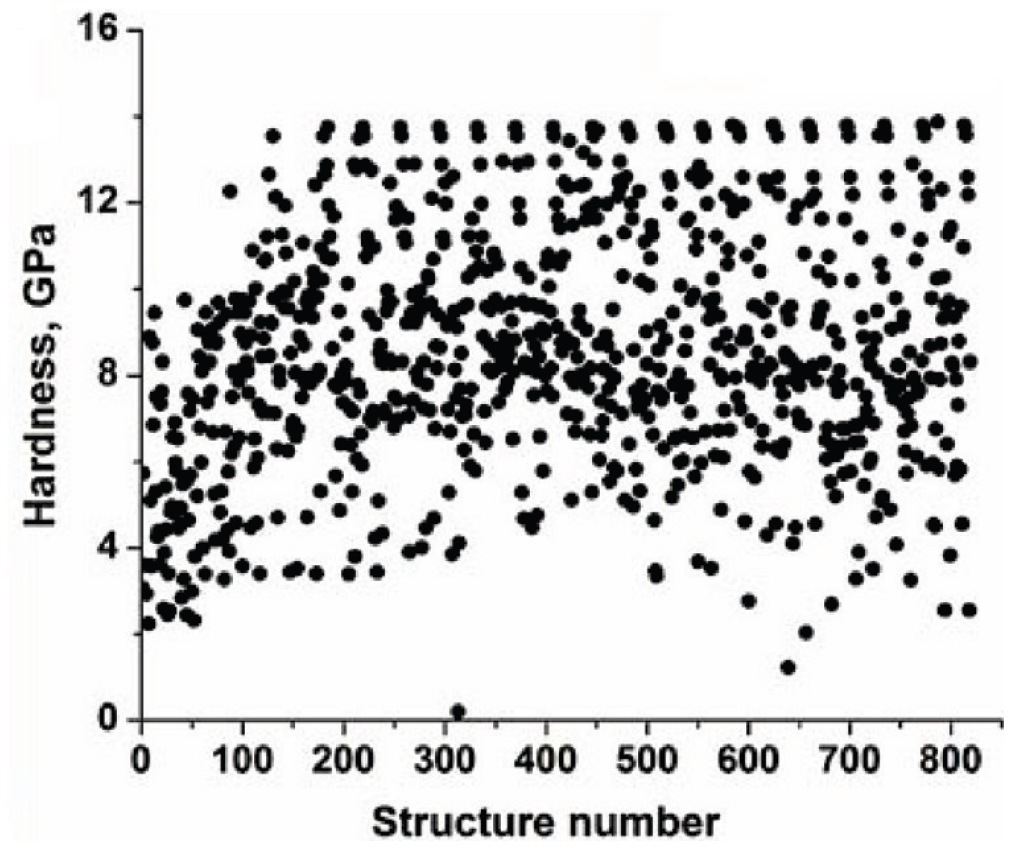
\includegraphics[scale=0.18]{pic/hardness_example}
\caption{\footnotesize \textbf{Predictions of the hardest structure of TiO$_2$.}}
\label{fig:hardness_example}
\end{figure}

\vspace{0.5cm}

Now, you need to specify what you know about the system.

% PPPPPPPPPPPPPPPPPPPPPPPPP
\paramacro{atomType}{Describes the identities of each type of atom.}{}{\rm none,
must specify explicitly}{\textshiftleft{\rm If you prefer to use the atomic
numbers from Mendeleev's Periodic Table of the Elements, specify:}
\% atomType \\
12 14 8 \\
\% EndAtomType}{Or, if you prefer to use atomic names, specify:

\textshift{\% atomType \\
Mg Si O \\
\% EndAtomType
}

You can alternatively specify the full names of the elements, for example:

\textshift{\% atomType \\
Magnesium Silicon Oxygen \\
\% EndAtomType
}}{}


%PPPPPPPPPPPPPPPPPPPPPPPPP
\paramacro{numSpecies}{Describes the number of atoms of each type.}{}{\rm none,
must specify explicitly}{\% numSpecies \\
4 4 12 \\
\% EndNumSpecies}{
This means there are 4 atoms of the first type, 4 of the second type, and 12 of
the third type.

\textbf{Notes:} For variable-composition calculations, you have to specify the
compositional building blocks as follows:

\textshift{\% numSpecies \\
2 0 3 \\
0 1 1 \\
\% EndNumSpecies
}{}

This means that the first building block has formula A$_2$C$_3$ and the second
building block has formula BC, where A, B and C are described in the block
\keyword{atomType}. All structures will then have the formula $x$A$_2$C$_3$ +
$y$BC with $x$, $y$ = (0,1,2,\ldots) --- or A$_{2x}$B$_y$C$_{3x+y}$. If you want
to do prediction of all possible compositions in the A-B-C system, you should
specify:

\textshift{\% numSpecies \\
1 0 0 \\
0 1 0 \\
0 0 1 \\
\% EndNumSpecies
}

You can also do fixed-composition calculations with a variable number of formula
units; in this case set just one line (and \keyword{calculationType}=301), for
example for compound A$_2$BC$_4$:

\textshift{\% numSpecies \\
2 1 4 \\
\% EndNumSpecies
}
}


%PPPPPPPPPPPPPPPPPPPPPPPPP
\paramacro{ExternalPressure}{Specifies external pressure at which you want to
find structures, in GPa.}{} {0}{100 : ExternalPressure}{\textbf{Note:} As of
USPEX 9.4.1 pressure value (in GPa) is set by the tag \keyword{ExternalPressure}
in the \file{INPUT.txt} file. Please NO LONGER specify it in relaxation files in
the \file{Specific/} folder.}


%PPPPPPPPPPPPPPPPPPPPPPPPP
\paramacro{valences}{Describes the valences of each type of atom. Used only to
evaluate bond hardnesses, which are used for computing the approximate dynamical
matrix (for softmutation) and hardness of the crystal.}{}{\rm USPEX has a table
of default valences (see Appendix~\ref{appendix_valences}). Beware, however,
that for some elements (\emph{e.g.}, N, S, W, Fe, Cr, \emph{etc.}) many valence
states are possible. Unless you calculate hardness, this is not a problem and
you can use the default values. If you do calculate the hardness, you need to
carefully specify the valence explicitly.
}{\% valences \\
2 4 2 \\
\% EndValences }{}


% PPPPPPPPPPPPPPPPPPPPPPPPP
\paramacro{goodBonds}{Specifes, in the matrix form, the minimum bond valences
for contacts that will be considered as important bonds. Like the
\keyword{IonDistances} matrix (see below), this is a square matrix cast in an
upper-triangular form. This is only used in calculations of hardness and in
softmutation. One can estimate these values for a given bond type taking
\keyword{goodBonds}=$\frac{valence}{max\_coordination\_number}$ or slightly
smaller.}{}{\rm USPEX can make a reasonable default estimation of
\keyword{goodBonds}, you will see the values in \file{OUTPUT.txt} file. This
should be sufficient for most purposes, but for hardness calculations you may
need to carefully examine these values and perhaps set them manually. For more
details, see Appendix~\ref{appendix_goodbonds}
}{\% goodBonds \\
10.0 10.0  0.2 \\
 0.0 10.0  0.5 \\
 0.0  0.0 10.0 \\
\% EndGoodBonds }
{\textbf{Notes:} The dimensions of this matrix must be equal to either the
number of atomic species or unity. If only one number is used, the matrix is
filled with this number. The matrix above reads as follows: to be considered a
bond, the Mg--Mg distance should be short enough to have bond valence of 10 or
more, the same for Mg--Si, Si--Si, and O--O bonds (by using such exclusive
criteria, we effectively disregard these interactions from the softmutation and
hardness calculations), whereas Mg--O bonds that will be considered for hardness
and softmutation calculations will have a bond valence of 0.2 or more, and the
Si--O bonds will have a bond valence of 0.5 or more.}


% PPPPPPPPPPPPPPPPPPPPPPPPP
\paramacro{checkMolecules}{Switches on/off post-relaxation check that original
molecules (files \file{MOL\_1}, \file{MOL\_2}, \ldots) are intact. Useful for
molecular crystals (\keyword{calculationType}=310, 311).}{Possible values
(integer):
\begin{itemize}
\item 0 --- check is not performed, structures with broken or merged molecules
are considered. (We strongly suggest users not to use this.)
\item 1 --- check is performed, all the structures with broken or merged
molecules are discarded.
\end{itemize}}{1}{1 : checkMolecules}{}


% PPPPPPPPPPPPPPPPPPPPPPPPP
\paramacro{checkConnectivity}{Switches on/off hardness calculation and
connectivity-related criteria in softmutation.}{Possible values (integer):
\begin{itemize}
\item 0 --- connectivity is not checked, no hardness calculations;
\item 1 --- connectivity is taken into account, hardness is calculated.
\end{itemize}
}{0}{1   : checkConnectivity}{}



\subsection{Population}

% PPPPPPPPPPPPPPPPPPPPPPPPP
\paramacro{populationSize}{The number of structures in each generation; initial
generation can be set separately, if needed.}{}{\rm $2 \times N$ rounded to the
closest 10, where $N$ is the number of atoms/cell (or \keyword{maxAt} for
variable composition). The upper limit is 60. Usually, you can trust these
default settings.}{20 : populationSize}{}


% PPPPPPPPPPPPPPPPPPPPPPPPP
\paramacro{initialPopSize}{The number of structures in the initial generation.}{
}{\rm equal to \keyword{populationSize}.}{20 : initialPopSize}{
\textbf{Note:}
In most situations, we suggest that these two parameters be equal. Sometimes
(especially in variable-composition calculations) it may be useful to specify
\keyword{initialPopSize} to be larger than \keyword{populationSize}. It is also
possible to have a smaller initial population, and this is useful if one wants
to generate the first population entirely from a few seed structures.}


% PPPPPPPPPPPPPPPPPPPPPPPPP
\paramacro{numGenerations}{Maximum number of generations allowed for the
simulation. The simulation can terminate earlier, if the same best structure
remains unchanged for \keyword{stopCrit} generations.}{}{100}{50 :
numGenerations}{}


% PPPPPPPPPPPPPPPPPPPPPPPPP
\paramacro{stopCrit}{The simulation is stopped if the best structure did not
change for stopCrit generations, or when \keyword{numGenerations} have expired
--- whichever happens first.}{}{\rm total number of atoms for fixed-composition
runs, maximum number of atoms \keyword{maxAt} for variable-composition runs.}{20
: stopCrit}{}

\subsection{Survival of the fittest and selection}


% PPPPPPPPPPPPPPPPPPPPPPPPP
\paramacro{bestFrac}{Fraction of the current generation that shall be used to
produce the next generation.}{}{0.7}{0.7 : bestFrac}{\textbf{Note:} This is an
important parameter, values between 0.5--0.8 are reasonable.}


% PPPPPPPPPPPPPPPPPPPPPPPPP
\paramacro{keepBestHM}{Defines how many best structures will survive into the
next generation.}{}{0.15$\times$\keyword{populationSize}}{3 : keepBestHM}{}

\paramacro{reoptOld}{Defines reoptimization of the survived structures. If
\keyword{reoptOld}=0, these structures will be left without reoptimization while
if \keyword{reoptOld}=1, they will be reoptimized again. Usually
\keyword{reoptOld}=0 is a reasonable choice (provided your structure relaxation
was high quality).}{}{0}{1 : reoptOld}{}


\subsection{Structure generation and variation operators}

% PPPPPPPPPPPPPPPPPPPPPPPPP
\paramacro{symmetries}{Possible space groups for crystals, plane groups for 2D
crystals/surfaces, or point groups for clusters. A certain number of structures
will be produced using randomly selected groups from this list, using randomly
generated lattice parameters and atomic coordinates. During this process special
Wyckoff sites can be produced from general positions
(Fig.~\ref{fig:Wyckoff_positions}).}{}{\begin{itemize} \item {\rm For 3D
crystals:} 2-230
\item {\rm For 2D crystals/surfaces:} 2-17 \item {\rm For clusters:} E C2 D2 C4
C3 C6 T S2 Ch1 Cv2 S4 S6 Ch3 Th Ch2 Dh2 Ch4 D3 Ch6 O D4 Cv3 D6 Td Cv4 Dd3 Cv6 Oh
Dd2 Dh3 Dh4 Dh6 Oh C5 S5 S10 Cv5 Ch5 D5 Dd5 Dh5 I Ih
\end{itemize}
}{\% symmetries \\
195-198 200 215-230 \\
\% EndSymmetries}{}

\begin{figure}[h]
\centering
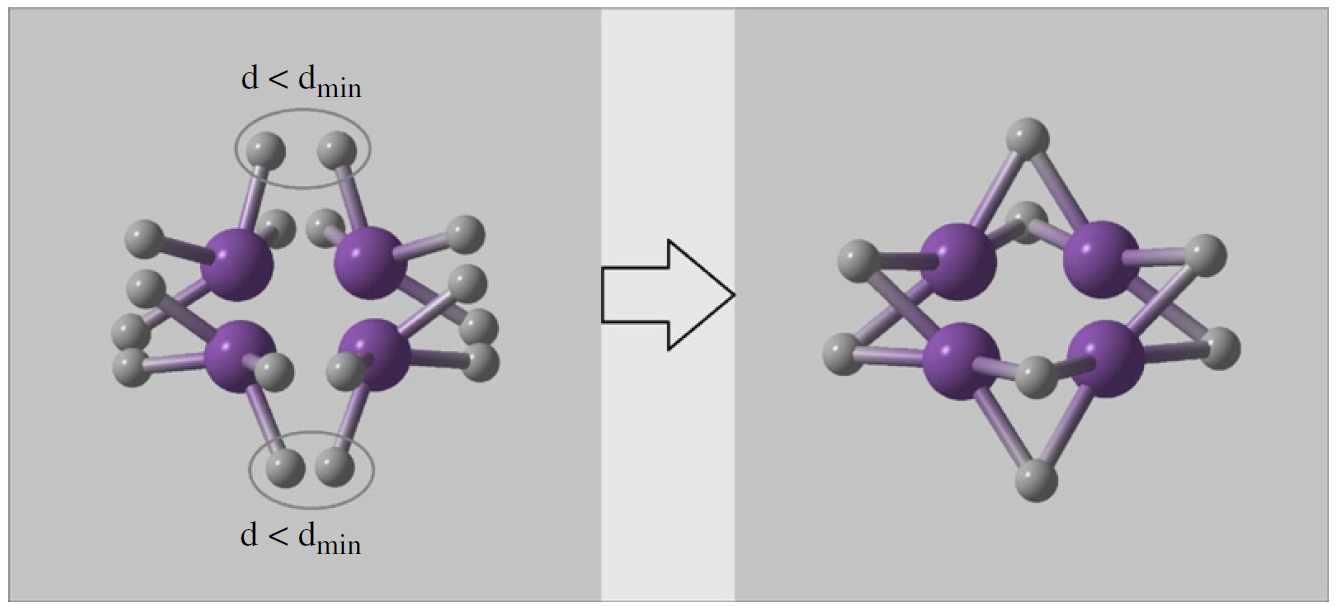
\includegraphics[scale=0.3]{pic/Wyckoff_positions}
\caption{\footnotesize \textbf{Example of merging atoms onto special Wyckoff
positions (from Ref. \cite{Lyakhov2013}).}}
\label{fig:Wyckoff_positions}
\end{figure}


% PPPPPPPPPPPPPPPPPPPPPPPPP
\paramacro{fracGene}{Percentage of structures obtained by heredity; 0.1 means
10\%, \emph{etc}.}{}{0.5}{0.5 : fracGene}{}\label{fracGene}


% PPPPPPPPPPPPPPPPPPPPPPPPP
\paramacro{fracRand}{Fraction of the generation produced randomly from the space
groups specified by the user.}{}{0.2}{0.20  : fracRand}{}\label{fracRand}


% PPPPPPPPPPPPPPPPPPPPPPPPP
\paramacro{fracPerm}{Percentage of structures obtained by permutation; 0.1 means
10\%, \emph{etc.}}{}{0.1 {\rm if there is more than one type of
atom/molecule;} 0 {\rm otherwise.}}{0.1   : fracPerm}{}


% PPPPPPPPPPPPPPPPPPPPPPPPP
\paramacro{fracAtomsMut}{Specifies the percentage of structures obtained by
softmutation or coormutation.}{}{0.1}{0.1   : fracAtomsMut}{\textbf{Note:} You
can use softmutation or coormutation by specifying \keyword{softMutTill}.}


% PPPPPPPPPPPPPPPPPPPPPPPPP
\paramacro{fracRotMut}{Percentage of structures obtained mutating molecular
orientations; 0.1 means 10\%, \emph{etc.}}{}{0.1 {\rm for molecular crystals;} 0
{\rm otherwise.}}{0.1   : fracRotMut}{}


% PPPPPPPPPPPPPPPPPPPPPPPPP
\paramacro{fracLatMut}{Percentage of structures obtained from lattice mutations;
0.1 means 10\%, \emph{etc.}}{}{0 {\rm for fixed cell prediction;} 0.1 {\rm
otherwise.}}{0.1 : fracLatMut}{\textbf{Note: If the sum of all the fractions
(\keyword{fracGene} + \keyword{fracRand} + \keyword{fracPerm} + \ldots) is not
equal to 1, they will be rescaled.}}

% PPPPPPPPPPPPPPPPPPPPPPPPP
\paramacro{howManySwaps}{For permutation, the number of pairwise swaps will be
randomly drawn from a uniform distribution between 1 and
\keyword{howManySwaps}.}{}{0.5$\times$\rm (maximum number of possible swaps).
{\rm If atoms $Na$ and $Nb$, and atoms $Nc$ and $Nd$ are swappable, then the
total number of possible swaps is $\min(Na,Nb)+\min(Nc,Nd)$, and the default for
\keyword{howManySwaps} is $0.5\times[\min(Na,Nb)+\min(Nc,Nd)]$. In most cases,
it is a good idea to rely on this default.}}{5     : howManySwaps}{}

% PPPPPPPPPPPPPPPPPPPPPPPPP
\paramacro{specificSwaps}{Specifies which atom types you allow to swap in
permutation.}{}{\rm blank line, which means no specific swaps and all atoms are
permutable.}{\% specificSwaps \\
1 2 \\
\% EndSpecific}{\textbf{Note:} In this case, atoms of type 1 could be swapped
with atoms of type 2. If you want to try all possible swaps, just leave a blank
line inside this keyblock, or delete the block.}


% PPPPPPPPPPPPPPPPPPPPPPPPP
\paramacro{mutationDegree}{The maximum displacement in softmutation in
$\text{\r{A}}$. The displacement vectors for softmutation or coormutation are
scaled so that the largest displacement magnitude equals
\keyword{mutationDegree}.}{}{3$\times${\rm (average atomic radius)}}{2.5   :
mutationDegree}{}


%PPPPPPPPPPPPPPPPPPPPPPPPP
\paramacro{mutationRate}{Standard deviation of the epsilons in the strain matrix
for lattice mutation. The strain matrix components are selected randomly from
the Gaussian distribution and are only allowed to take values between -1 and 1.
Lattice mutation essentially incorporates the ideas of metadynamics into our
method \cite{Oganov-book2010a, Martonak2005}, where new structures are found by
building up cell distortions of some known structure. Unlike in metadynamics,
the distortions are not accumulated in our method, so the strain components
should be large to obtain new structures.}{}{0.5}{0.5   : mutationRate}{}

\vspace{0.5cm}

It is a good idea to combine lattice mutation with a weak softmutation:


%PPPPPPPPPPPPPPPPPPPPPPPPP
\paramacro{DisplaceInLatmutation}{Specifies softmutation as part of lattice
mutation and sets the maximum displacement in $\text{\r{A}}$.}{}{1.0}{1.0   :
DisplaceInLatmutation}{}

\paramacro{AutoFrac}{Enables automatic evolution of variation operators
(parameter control), which speeds up the calculation by up to $\sim$2 times. To
switch to user defined variation operators, set \keyword{AutoFrac}=0.}{}{0}{1 :
AutoFrac}{}


\subsection{Constraints}

The same structure can be represented in an infinite number of coordinate
systems (``modular invariance''). Most of these equivalent choices will lead to
very flat unit cells, which creates problems for structure relaxation and energy
calculation (\emph{e.g.}, a very large number of $k$-points are needed). The
constraint, well known in crystallography, that the cell angles be between
60$^\circ$ and 120$^\circ$, does not remove all redundancies and problematic
cells (\emph{e.g.}, thus allowed cells with $\alpha=\beta=\gamma \sim 120^\circ$
are practically flat). Therefore, we developed \cite{Oganov2008,
Oganov-book2010b} a special scheme to obtain special cell shapes with the
shortest cell vectors. This transformation can be performed if there is at least
one lattice vector whose projection onto any other cell vector or the diagonal
vector of the opposite cell face is greater (by modulus) than half the length of
that vector, \emph{i.e.}, for pairs $\textbf{a}$ and $\textbf{b}$, or
$\textbf{c}$ and $(\textbf{a}+\textbf{b})$ these criteria are:

\begin{eqnarray}\label{eq:cellCons}
\left|\frac{\bf a \cdot b}{\bf \vert b \vert}\right| &>& \frac{\bf |b|}{2} \label{eq:cellCons1}\\
\left|\frac{\bf a \cdot b}{\bf \vert a \vert}\right| &>& \frac{\bf |a|}{2} \label{eq:cellCons2}\\
\left|\frac{\bf c \cdot (a + b)}{\bf \vert c \vert}\right| &>& \frac{\bf |c|}{2} \label{eq:cellCons3}\\
\left|\frac{\bf c \cdot (a + b)}{\bf \vert a+b \vert}\right| &>& \frac{\bf |a+b|}{2} \label{eq:cellCons4}
\end{eqnarray}

For instance, for the criterion \ref{eq:cellCons1} the new vector $\bf a^*$
equals:

\begin{equation}
{\bf a}^* = {\bf a} - {\rm ceil} \left( \frac{\vert {\bf a} \cdot {\bf b}
\vert}{\vert {\bf b} \vert ^2} \right){\rm sign}({\bf a}\cdot {\bf b}){\bf b}
\end{equation}

This transformation is performed iteratively, completely avoids pathological
cell shapes, and thus solves the problem. During this transformation, the atomic
fractional coordinates are transformed so that the original and transformed
structures are identical (during the transformation, the Cartesian coordinates
of the atoms remain invariant).


% PPPPPPPPPPPPPPPPPPPPPPPPP
\paramacro{minVectorLength}{Sets the minimum length of a cell parameter of a
newly generated structure.}{}{\rm 1.8 $\times$ covalent diameter of the largest
atom. For molecular crystals \\(\keyword{calculationType} = 310, 311) default
value is 1.8 $\times$ max(\keyword{MolCenters}).}{2.0 : minVectorLength}{}

\vspace{0.5cm}

Commonly used computational methods (pseudopotentials, PAW, LAPW, and many
parametric forcefields) break down when the interatomic distances are too small.
This situation needs to be avoided and you can specify the minimum distances
between each pair of atoms using the \keyword{IonDistances} square matrix cast
in an upper-triangular form:


% PPPPPPPPPPPPPPPPPPPPPPPPP
\paramacro{IonDistances}{Sets the minimum interatomic distance matrix between
different atom types. Distances lower than \keyword{IonDistances} are considered
entirely unphysical and will be strictly avoided.}{} {\rm the
\keyword{IonDistances} between atom A and B are estimated as
$0.2\times(V_{A}^{1/3}+V_{B}^{1/3})$ but not larger then 1.2~$\text{\r{A}}$, and
$0.45\times(V_{A}^{1/3}+V_{B}^{1/3})$ in molecular calculations, where $V_A$ and
$V_B$ are the default volumes of atom \emph{A} and \emph{B} estimated in USPEX.
}{\% IonDistances\\
1.0 1.0 0.8 \\
0.0 1.0 0.8 \\
0.0 0.0 1.0 \\
\% EndDistances}{
\textbf{Note:} The dimensions of this matrix must be equal to the number of
atomic species. If the compound in the example above is MgSiO$_3$, the matrix
reads as follows: the minimum Mg--Mg distance allowed in a newly generated
structure is 1.0~$\text{\r{A}}$, the minimum Mg--Si, Si--Si and O--O distances
are also 1.0~$\text{\r{A}}$, and the minimum Mg--O and Si--O distances are
0.8~$\text{\r{A}}$. You can use this keymatrix to incorporate further
system-specific information: \emph{e.g.}, if you know that Mg atoms prefer to be
very far apart and are never closer than 3~$\text{\r{A}}$ in your system, you
can specify this information. Beware, however, that the larger these minimum
distances, the more difficult it is to find structures fulfilling these
constraints (especially for large systems), so strive for a compromise and
remember that \keyword{IonDistances} must be \textbf{much} smaller than the
actual bond lengths.
}


% PPPPPPPPPPPPPPPPPPPPPPPPP
\paramacro{constraint\_enhancement}{Allows one to apply the stricter constraints
of the \keyword{IonDistances} matrix (by \keyword{constraint\_enhancement}
times) for symmetric random structures (for all variation operators, unenhanced
\keyword{IonDistances} matrix still applies). Only use it if you know what you
are doing.}{}{1}{1   :  constraint\_enhancement}{}

\vspace{0.5cm}

For molecular crystals, the following keyblock is extremely important:

% PPPPPPPPPPPPPPPPPPPPPPPPP
\paramacro{MolCenters}{Matrix of minimal distances between the centers of
molecules. Any distances lower than these indicate large overlap of the
molecules, are unphysical and will be strictly avoided.}{}{\rm zero-matrix for
non-molecular calculations, no default for molecular crystals (must specify
explicitly).}{\% MolCenters \\
5.5 7.7 \\
0.0 9.7 \\
\% EndMol}{
\textbf{Note:} In the above example, there are two types of molecules. In all of
the generated structures, the distance between the geometric centers of the
molecules of the first type must be at least 5.5~$\text{\r{A}}$ (A--A distance),
the distance between the centers of the molecules of the first and second type
--- 7.7~$\text{\r{A}}$ (A--B distance), and the distance between the molecules
of the second type --- 9.7~$\text{\r{A}}$ (B--B distance).}


\subsection{Cell} \label{input_cell}

It is useful to create all new structures (before relaxing them) with a unit
cell volume appropriate for given conditions. This can be specified in the
\keyword{Latticevalues} keyblock:

% PPPPPPPPPPPPPPPPPPPPPPPPP
\paramacro{Latticevalues}{Specifies the initial volume of the unit cell or known
lattice parameters.}{}{\rm For cell volumes you don't have to specify values ---
USPEX has a powerful algorithm to find reasonable estimates at any pressure.}
{\% Latticevalues \\
125.00 \\
\% Endvalues}{}


\textbf{Notes:} (1) This volume is only used as an initial guess and only
influences the first generation, each structure is fully optimized and adopts
the volume corresponding to the (free) energy minimum. This keyblock also has
another use: when you know the lattice parameters (\emph{e.g.}, from
experiment), you can specify them in the \keyword{Latticevalues} keyblock
instead of unit cell volume, \emph{e.g.}:

\textshift{\% Latticevalues \\ 
7.49 0.0 0.0 \\
0.0 9.71 0.0 \\
0.0 0.0 7.07 \\
\% Endvalues
}

You can also specify unit cell parameters just by listing \keyword{a},
\keyword{b}, \keyword{c}, $\alpha$, $\beta$, and $\gamma$ values:

\textshift{\% Latticevalues \\ 
10.1 8.4 12.5 90.0 101.3 90.0 \\
\% Endvalues
}

Attention: if you do a calculation with a fixed monoclinic cell, please use
setting with special angle $\beta$ (standard setting).

(2) For variable-composition calculations, you have to specify the volume of
end members of the compositional search space, \emph{e.g.}:

\textshift{\% Latticevalues \\
12.5 14.0 11.0 \\
\% Endvalues 
}

(3) Users no longer need to specify the unit cell or atomic volumes in the
keyblock \keyword{Latticevalues} --- a special algorithm has been implemented
that accurately estimates it at the pressure of interest, without the need for
the user to specify it. This option works well and is available for any
\keyword{calculationType} where input volumes are required: 3**, 2D-crystals,
110, 000. You can also use online program
\textcolor{blue}{\url{http://han.ess.sunysb.edu/volume_estimation}}. The users
can also input the volumes manually.

(4) If you study molecular crystals under pressure, you might sometimes need to
increase the initial volumes somewhat, in order to be able to generate
structures by the random symmetric algorithm.


% PPPPPPPPPPPPPPPPPPPPPPPPP
\paramacro{splitInto}{Defines the number of identical subcells or pseudosubcells
in the unit cell. If you do not want to use splitting, just use the value 1, or
delete the block. Use splitting only for systems with
$>$25--30~atoms/cell.}{}{1}
{\% splitInto (number of subcells into which the unit cell is split) \\
1 2 4 \\
\% EndSplitInto}{}

Subcells introduce extra translational (pseudo)symmetry. In addition to this,
each subcell can be built using a special space groups algorithm developed by
A.R.~Oganov and H.T.~Stokes and implemented by H.T.~Stokes (see Reference
\cite{Lyakhov2013}).


\subsection{Restart} \label{input_restart}

If something goes wrong, you may want to continue the calculation from the point
where it stopped --- or from an earlier point. If all you want to do is
continue the run from where it stopped, you do not need to change any settings
(all information will be stored in the \file{*.mat} files) and it will be
sufficient to remove the file \file{still\_reading} and run USPEX again.

If you want to restart from a particular generation in a particular
\file{results}-folder, then specify \keyword{pickUpGen} = number of the
generation from which you want to start, \file{pickUpFolder} = number of
\file{results}-folder (\emph{e.g.}, 1 for \file{results1}, 2 for
\file{results2}, \ldots) from which the restart needs to be initiated. If
\keyword{pickUpGen}=0, then a new calculation is started. The default options
for all three parameters are 0. For example, to restart a calculation performed
in the folder \file{results5} from generation number 10, specify:

\textshift{10    : pickUpGen \\
5     : pickUpFolder \\ 
}



\subsection{Details of \emph{ab initio} calculations}

USPEX employs a powerful two-level parallelization scheme, making its parallel
scalability exemplary. The first level of parallelization is performed within
structure relaxation codes, the second level of parallelization distributes the
calculation over the individuals in the same population (since structures within
the same generation are independent of each other).

First, you must specify which code(s) you want to use for structure relaxation
and fitness calculation:

% PPPPPPPPPPPPPPPPPPPPPPPPP
\paramacro{abinitioCode}{Defines the code used for every optimization step.}{}{1
{\rm for every optimization step (VASP)}}{\% abinitioCode \\
3 2 2 1 1 \\
\% ENDabinit}{
\textbf{Note:} Numbers indicate the code used at each step of structure
relaxation (see Subsection~\ref{abinitio_codes} for a list of supported codes):

\begin{multicols}{2}
\begin{itemize}
\item[] \texttt{ 1} --- VASP
\item[] \texttt{ 2} --- SIESTA
\item[] \texttt{ 3} --- GULP
\item[] \texttt{ 4} --- LAMMPS
\item[] \texttt{ 5} --- Neural Networks code \\
(unused at the moment)
\item[] \texttt{ 6} --- DMACRYS
\item[] \texttt{ 7} --- CP2K
\item[] \texttt{ 8} --- Quantum Espresso
\item[] \texttt{ 9} --- FHI-aims
\item[] \texttt{10} --- ATK
\item[] \texttt{11} --- CASTEP
\item[] \texttt{12} --- Tinker
\item[] \texttt{13} --- MOPAC
\end{itemize}
\end{multicols}
}

% PPPPPPPPPPPPPPPPPPPPPPPPP
\paramacro{KresolStart}{Specifies the reciprocal-space resolution for $k$-points
generation (units: $2\pi\text{\r{A}}^{-1}$).}{}{\rm from 0.2 to 0.08 linearly}{
\% KresolStart \\
0.2 0.16 0.12 0.08 \\
\% Kresolend}{
\textbf{Note:} You can enter several values (one for each step of structure
relaxation), starting with cruder (\emph{i.e.}, larger) values and ending with
high resolution. This dramatically speeds up calculations, especially for
metals, where very many \emph{k}-points are needed. This keyblock is important
if you use VASP or QuantumEspresso (with GULP it is not needed at all, and with
SIESTA you will have to define \keyword{KresolStart} within SIESTA input
files).}


\vspace{0.5cm}
For \textbf{clusters}, \textbf{2D-crystals}, and \textbf{surfaces}, you have to
specify the thickness of the vacuum region around the cluster (or around the
surface slab):

% PPPPPPPPPPPPPPPPPPPPPPPPP
\paramacro{vacuumSize}{Defines the amount of vacuum added around the structure
(closest distance in $\text{\r{A}}$ between neighboring clusters in adjacent
unit cells). Used only for surfaces, 2D-crystals, and nanoparticles.}{}{10 {\rm
$\text{\r{A}}$ for every step of relaxation}}{\% vacuumSize \\
10 10 15 20 20 \\
\% EndVacuumSize}{}


% PPPPPPPPPPPPPPPPPPPPPPPPP
\paramacro{numParallelCalcs}{Specifies how many structure relaxations you want
to run in parallel.}{}{1}{10   : numParallelCalcs}{}

You need to supply the job submission files or the names of executable files for
each code/mode you are using.


% PPPPPPPPPPPPPPPPPPPPPPPPP
\paramacro{commandExecutable}{Specifies the name of the job submission files or
executables for a given code.}{}{\rm no default, has to be specified by the
user.}{\% commandExecutable \\
gulp < input > output \\
mpirun -np 8 vasp > out \\
mpirun -np 8 vasp > out \\
mpirun -np 8 vasp > out \\
\% EndExecutable}{\textbf{Note:} Every line corresponds to a stage of relaxation
--- the first line describes the execution of the first stage of relaxation,
\emph{etc}. For example, \keyword{abinitioCode} equal to ``\texttt{3 1 1 1}''
means that the first relaxation step will be performed with GULP, while the
subsequent steps will be performed using VASP via the command ``\texttt{mpirun
-np 8 vasp > out}''. If only one line is present in \keyword{commandExecutable},
then the same execution will be performed for all steps of relaxation.}

\vspace{0.5cm}

You can actually use USPEX on virtually any platform in the remote submission
mode. All you need is MATLAB/Octave to be running on your workstation. In that
case, your workstation will prepare input (including jobs), send them to the
remote compute nodes, check when the calculations are complete, get the results
back, analyze them, and prepare new input. The amount of data being sent to and
fro is not large, so the network does not need to be very fast. Job submission
is, of course, machine-dependent.

% PPPPPPPPPPPPPPPPPPPPPPPPP
\paramacro{whichCluster}{Specifies the types of job submission.}{
Possible values (integer):
\begin{itemize}
\item 0 --- no-job-script;
\item 1 --- local submission;
\item 2 --- remote submission.
\end{itemize}}{0}{1     : whichCluster}{}


\paramacro{remoteFolder}{Folder on the remote supercomputer where the
calculation will be performed. This keyword is activated only if
\keyword{whichCluster}=2.}{}{\rm none}{Blind\_test  : remoteFolder}{
\textbf{Note:} there is a similar parameter specified in the remote submission
file --- \keyword{homeFolder}. The actual path to the calculation will be
\file{*homeFolder*/*remoteFolder*/CalcFolderX} where \texttt{X}=1, 2, 3,\ldots.}


\paramacro{PhaseDiagram}{Enables calculation of a phase diagram for
\keyword{calculationType}=300 and 301. It gives an idea (crude one --- just to
get a rough idea!) of which the new phases may be at higher and lower pressures,
and a rough idea of transition pressures.}{} {0}{1 : PhaseDiagram}{}


\subsection{Fingerprint settings} \label{input_fingerprints}

Before changing the following parameters, we encourage you to read the
methodological papers first, so you understand what you are doing (Oganov \&
Valle, 2009 \cite{Oganov2009}).

\paramacro{RmaxFing}{The distance cutoff (in $\text{\r{A}}$).}{}{10.0}{10.0  :
RmaxFing}

\paramacro{deltaFing}{The discretization (in $\text{\r{A}}$) of the fingerprint
function.}{}{0.08}{0.10  : deltaFing}

\paramacro{sigmaFing}{The Gaussian broadening of interatomic distances.}{}{0.03}
{0.05  : sigmaFing}

\keyword{toleranceFing} (default=0.008) and \keyword{toleranceBestHM}
(default=0.02) specify the minimal cosine distances between structures that
qualify them as non-identical --- for participating in the production of child
structures and for survival of the fittest, respectively. They depend on the
precision of structure relaxation and the physics of the system (for instance:
for ordering problems, fingerprints belonging to different structures will be
very similar, and these tolerance parameters should be made small).
\keyword{toleranceBestHM} is used only if \keyword{dynamicalBestHM}=1 (which we
don't use anymore), so this parameter is essentially obsolete.


\subsection{Antiseed settings}

A family of antiseed techniques have been developed and implemented in USPEX,
all based on the idea of penalizing already sampled structures to ensure that
the simulation is not stuck in a local minimum. Here, time-dependent fitness is
the sum of the actual enthalpy (or another fitness property of interest) and a
history-dependent term, which is the sum of the Gaussian potentials added to
already sampled parts of the energy landscape:
\[ f=f_0 + \sum_{a} W_a \exp \left(-\frac{d_{ia}^{2}}{2\sigma_{a}^{2}}\right),
\] where $f$ is fitness ($f_0$ --- the true fitness, $f$ --- history-dependent
fitness), $W_a$ is the height and $\sigma_{a}$ is the width of the Gaussian. In
our approach, Gaussian parameters change depending on the population diversity
and energy spread at each generation.

There are three ways to use this technique. In the first, you can put the
structure that you wish to penalize in the \file{AntiSeeds} folder. For example,
this can be the ground state structure --- in this case, USPEX will try to find
the second lowest-enthalpy structure.

In the second and third methods, you don't specify antiseed structure(s) --- the
calculation either uses all sampled structures as antiseeds (well tested; the
recommended approach) or just the best structure in each generation.
You need to specify a few settings:

% PPPPPPPPPPPPPPPPPPPPPPPPP
\paramacro{antiSeedsActivation}{Specifies from which generation the antiseed
mode will be switched on. When antiSeedsActivation $= N > 0$, Gaussians are
added to all structures starting from generation $N$, and when $N<0$ ---
Gaussians are only added to the best structure of each generation, starting from
generation $N$. When $N=0$, Gaussians are only added to the structures put in
the \file{AntiSeeds} folder. If you don't want to use antiseeds, specify very
large \keyword{antiSeedsActivation} (for example, 5000) and
\keyword{antiSeedsMax}=0.0.}{}{5000}{1 : antiSeedsActivation }{}



% PPPPPPPPPPPPPPPPPPPPPPPPP
\paramacro{antiSeedsMax}{Specifies the height of the Gaussian, in units of the
mean square deviation of the enthalpy in the generation (computed only among
\keyword{bestFrac} structures, \emph{i.e.}, among potential parents). We
recommend \keyword{antiSeedsMax}=0.01.}{}{0.000}{0.005 : antiSeedsMax}{}



% PPPPPPPPPPPPPPPPPPPPPPPPP
\paramacro{antiSeedsSigma}{Specifies the width of the Gaussian, in units of the
average distance between structures in the generation (computed only among
\keyword{bestFrac} structures, \emph{i.e.}, among potential parents). We
recommend \keyword{antiSeedsSigma}=0.005.}{}{0.001}{0.005 : antiSeedsSigma}{}

\vspace{0.5cm}

Fig.~\ref{fig:antiseeds} shows an example of use of antiseed technique.

\begin{figure}[h] \centering 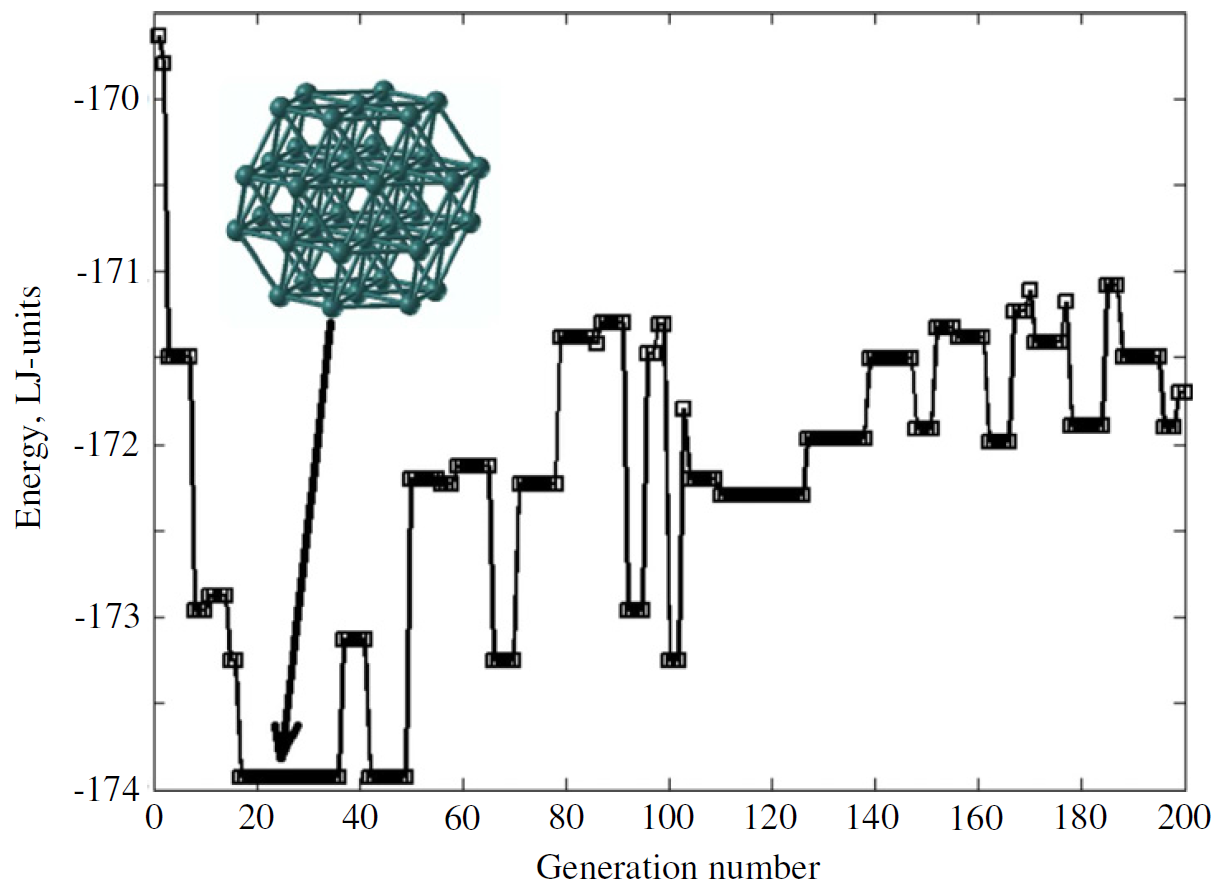
\includegraphics[scale=0.3]{pic/antiseeds}
\caption{\footnotesize \textbf{Example of a calculation of a Lennard-Jones
cluster with 38 atoms with the use of antiseeds.} The energy of the best
structure in every generation is plotted. One can clearly see that the algorithm
does not get stuck for a long time to any of the candidate minima and quickly
finds the ground state. Here we used \keyword{antiSeedsActivation}=1,
\keyword{antiSeedsMax}=0.01, \keyword{antiSeedsSigma}=0.001.}
\label{fig:antiseeds}
\end{figure}


\subsection{Space group determination} \label{input_space_groups}

% PPPPPPPPPPPPPPPPPPPPPPPPP
\paramacro{doSpaceGroup}{Determines space groups and also writes output in the
crystallographic \file{*.CIF}-format (this makes your life easier when preparing
publications, but beware that space groups may sometimes be under-determined if
the relaxation was not very precise and if very stringent tolerances were set
for the symmetry finder). This option is enabled thanks to the powerful symmetry
code provided by H.T.~Stokes.}{}{1, {\rm if} \keyword{calculationType}=3** {\rm
(\texttt{300}, \texttt{301}, \texttt{310}, \texttt{311} --- bulk crystals) and}
0 {\rm otherwise.}}{1 : doSpaceGroup (0 - no space groups, 1 - determine space
groups)}{}


% PPPPPPPPPPPPPPPPPPPPPPPPP
\paramacro{SymTolerance}{Precision for symmetry determination using the symmetry
finder code of H.T. Stokes. Can be specified either as a number (in
$\text{\r{A}}$) or as \texttt{high | medium | low}
(= \texttt{0.05 | 0.10 | 0.20})}{} {medium}{medium : SymTolerance}{}



\subsection{Keywords for developers}

\paramacro{repeatForStatistics}{Number of automatically executed USPEX runs.
USPEX simulations are stochastic, and redoing the simulation with the same input
parameters does not necessarily yield the same results. While the final result
--- the ground state --- is the same (hopefully!), the number of steps it takes
to reach it and the trajectory in chemical space differ from run to run. To
compare different algorithms, you MUST collect some statistics --- do not rely
on just a single run (which may be lucky or unlucky\ldots USPEX does not rely on
luck!). This option is only of interest to developers and it only makes sense to
collect statistics with simple potentials (\emph{e.g.}, using GULP). }{}{1 {\rm
(\emph{i.e.}, no statistics will be gathered)}}{20 : repeatForStatistics}{}

\paramacro{stopFitness}{Specifies the fitness value so that the calculation will
stop after reaching fitness $\leq$ \keyword{stopFitness}.}{}{\rm no default, has
to be specified by the user.}{90.912 : stopFitness}{}

\textbf{Note:} Automatic analysis of statistics is enabled when
\keyword{stopFitness} is specified. It is recommended to set
\keyword{repeatForStatistics} keyword to values $>$1 to collect the statistics
of reachability of \keyword{stopFitness}. Sample output is:

{\tiny
\begin{verbatim}
	Number of files to be processed: 20
	Target enthalpy: 90.912

	Generation: 23    Number: 1326    Enthalpy:    90.9119    Mat-file: /home/USPEX/01/results1/USPEX.mat
	Generation: 22    Number: 1224    Enthalpy:    90.9119    Mat-file: /home/USPEX/02/results1/USPEX.mat
	Generation: 60    Number: 3451    Enthalpy:    90.9119    Mat-file: /home/USPEX/03/results1/USPEX.mat
	Generation: 30    Number: 1739    Enthalpy:    90.9119    Mat-file: /home/USPEX/04/results1/USPEX.mat
	Generation: 17    Number:  956    Enthalpy:    90.9119    Mat-file: /home/USPEX/05/results1/USPEX.mat
	Generation: 36    Number: 2055    Enthalpy:    90.9119    Mat-file: /home/USPEX/06/results1/USPEX.mat
	Generation: 35    Number: 1987    Enthalpy:    90.9119    Mat-file: /home/USPEX/07/results1/USPEX.mat
	Generation: 22    Number: 1241    Enthalpy:    90.9119    Mat-file: /home/USPEX/08/results1/USPEX.mat
	Generation: 18    Number: 1002    Enthalpy:    90.9119    Mat-file: /home/USPEX/09/results1/USPEX.mat
	Generation: 29    Number: 1641    Enthalpy:    90.9119    Mat-file: /home/USPEX/10/results1/USPEX.mat
	Generation: 21    Number: 1197    Enthalpy:    90.9119    Mat-file: /home/USPEX/11/results1/USPEX.mat
	Generation: 27    Number: 1542    Enthalpy:    90.9119    Mat-file: /home/USPEX/12/results1/USPEX.mat
	Generation: 44    Number: 2519    Enthalpy:    90.9119    Mat-file: /home/USPEX/13/results1/USPEX.mat
	Generation: 32    Number: 1821    Enthalpy:    90.9119    Mat-file: /home/USPEX/14/results1/USPEX.mat
	Generation: 15    Number:  835    Enthalpy:    90.9119    Mat-file: /home/USPEX/15/results1/USPEX.mat
	Generation: 43    Number: 2477    Enthalpy:    90.9119    Mat-file: /home/USPEX/16/results1/USPEX.mat
	Generation: 40    Number: 2278    Enthalpy:    90.9119    Mat-file: /home/USPEX/17/results1/USPEX.mat
	Generation: 24    Number: 1358    Enthalpy:    90.9119    Mat-file: /home/USPEX/18/results1/USPEX.mat
	Generation: 14    Number:  757    Enthalpy:    90.9119    Mat-file: /home/USPEX/19/results1/USPEX.mat
	Generation: 27    Number: 1532    Enthalpy:    90.9119    Mat-file: /home/USPEX/20/results1/USPEX.mat

	Found structures numbers : 1326 1224 3451 1739  956 2055 1987 1241 1002 1641 1197 1542 2519 1821  835 2477 2278 1358  757 1532
	Found generations numbers:   23   22   60   30   17   36   35   22   18   29   21   27   44   32   15   43   40   24   14   27

	Success rate: 100 percent
	Average number of generations to get E=90.912: 29
	Average number of structures  to get E=90.912: 1647
	Standard deviation: 670
\end{verbatim}
}


\paramacro{collectForces}{Enable to collect all relaxation information in USPEX
calculation, including forces on the atoms, atomic positions, lattice parameters
and stress tensors during the structure optimizations. The information is stored
in \file{FORCE.mat} file. Only VASP is supported.}{}{0}{1 : collectForces}{}


\subsection{Seldom used keywords}

\paramacro{ordering\_active}{Switch on the biasing of variation operators by
local order parameters.}{}{1}{1 : ordering\_active}{}

\paramacro{symmetrize}{Switches on a transformation of all structures to
standard symmetry-adapted crystallographic settings.}{}{0}{1 : symmetrize}{}

\paramacro{valenceElectr}{Number of valence electrons for each type of
atoms.}{}{\rm these numbers are constants for all atoms, and we have
tabulated them, no need to specify explicitly.}{\% valenceElectr \\
2 6\\
\% EndValenceElectr}{}

\paramacro{percSliceShift}{Probability of shifting slabs (used in heredity) in
all dimensions, 1.0 means 100\%.}{}{1.0}{0.5 : percSliceShift}{}

% PPPPPPPPPPPPPPPPPPPPPPPPP
\paramacro{dynamicalBestHM}{Specifies whether the number of surviving best
structures will vary during the calculation, with \keyword{keepBestHM} as the
upper limit.

Possible values (integer): 0 = no variation, 1 and 2 = see note}{}{ 2 }{1 :
dynamicalBestHM}{}

\textbf{Note:} If you set \keyword{dynamicalBestHM}=1, the code will choose up
to \keyword{keepBestHM} lowest-energy structures (without duplicate structures,
which are defined as having fingerprint distance below user-defined
\keyword{toleranceBestHM}). If \keyword{dynamicalBestHM}=2 (our preferred
choice), then clustering algorithm selects exactly \keyword{keepBestHM}
maximally different structures in the entire energy interval corresponding to
\keyword{bestFrac}, and optimum \keyword{toleranceBestHM} is determined
automatically --- this promotes diversity while retaining memory of good
structures.


%PPPPPPPPPPPPPPPPPPPPPPPPP
\paramacro{softMutOnly}{How many generations should be produced by softmutation
only.}{}{0}{\% softMutOnly \\
1-5 \\
\% EndSoftOnly}{}

\textbf{Note:} In the example above, the generations up to 5$^{th}$ generation
(excluding, of course, the first generation) are produced by softmutation alone.
Note that upon softmutation, each parent produces TWO softmutants. You can also
specify particular generations to be softmutated throughout the run, for example
to softmutate every 10$^{th}$ generation you can write:
\begin{verbatim}
% softMutOnly 
2 12 22 32 42
% EndSoftOnly
\end{verbatim}


% PPPPPPPPPPPPPPPPPPPPPPPPP
\paramacro{maxDistHeredity}{Specifies the maximal cosine distances between
structures that participate in heredity. This specifies the radius on the
landscape within which structures can mate. Use with care (or do not use at
all).}{}{0.5}{0.5 : maxDistHeredity}{}


% PPPPPPPPPPPPPPPPPPPPPPPPP
\paramacro{manyParents}{Specifies whether more than two slices (or more than two
parent structures) should be used for heredity. This may be beneficial for very
large systems.}{

Possible values (integer): 

0 --- only 2 parents are used, 1 slice each.

1 --- many structures are used as parents, 1 slice each.

2 --- two structures are used as parents, many slices (determined dynamically
using parameters \keyword{minSlice} and \keyword{maxSlice}) are chosen
independently from each one.

3 --- two structures are used as parents, many slices (determined dynamically
using parameters \keyword{minSlice} and \keyword{maxSlice}) are cut from the
cell with a fixed offset. This is the preferred option for large systems. For
example, we cut both structures into slices of approximately the same thickness
and then choose the even slices from parent 1 and odd slices form parent 2,
making a multilayered ``sandwich'', or a ``zebra''.
}{0}{3 : manyParents }{}

\vspace{0.5cm}

\keyword{\color{blue} minSlice, maxSlice}: Determines the minimal and maximal
thickness of the slices in $\text{\r{A}}$ that will be cut out of the parent
structures to participate in creation of the child structure. We want the slices
to be thick enough to carry some information about the parent (but not too thick
to make heredity ineffective). Reasonable values for these parameters are around
1 and 6~$\text{\r{A}}$, respectively.

\vspace{0.5cm}

For clusters, you can directly specify the number of parents participating in
heredity (but we found this to be of little use):

%PPPPPPPPPPPPPPPPPPPPPPPPP
\paramacro{numberparents}{Defines the number of parents in heredity for
clusters.}{}{2}{2 : numberparents}{}



%%%%%%%%%%%%%%%%%%%%%%%%%%%%%%%%%%%%%%%%%%%%%%%%%%%%%%%%%%%%%%%%%%%%%%%%%%%%%%%%
\newpage
\section{Additional input for special cases}

\subsection{\file{MOL\_1}, \file{MOL\_2}, \ldots files for molecular crystals}
\label{molecular_crystals}
 
\subsubsection{Molecular Crystals, \keyword{calculationType}=310/311} 

For a molecular crystal, the \file{MOL\_1} file describes the structure of the
molecule from which the structure is built. This file also defines which torsion
angles will be mutated if the molecule is flexible. This file and its format
differ from SIESTA's \file{Z\_Matrix} file (\file{MOL\_1} gives the Cartesian
coordinates of the atoms, whereas \file{Z\_Matrix} file defines the atomic
positions from bond lengths, bond angles and torsion angles). The
\file{Z\_Matrix} file is created using the information given in the
\file{MOL\_1} file, \emph{i.e.}, bond lengths and all necessary angles are
calculated from the Cartesian coordinates. The lengths and angles that are
important should be used for the creation of \file{Z\_Matrix} --- this is
exactly what columns 5--7 specify. Let's look at the \file{MOL\_1} file for
benzene C$_6$H$_6$:

\begin{figure}[htbp] \centering
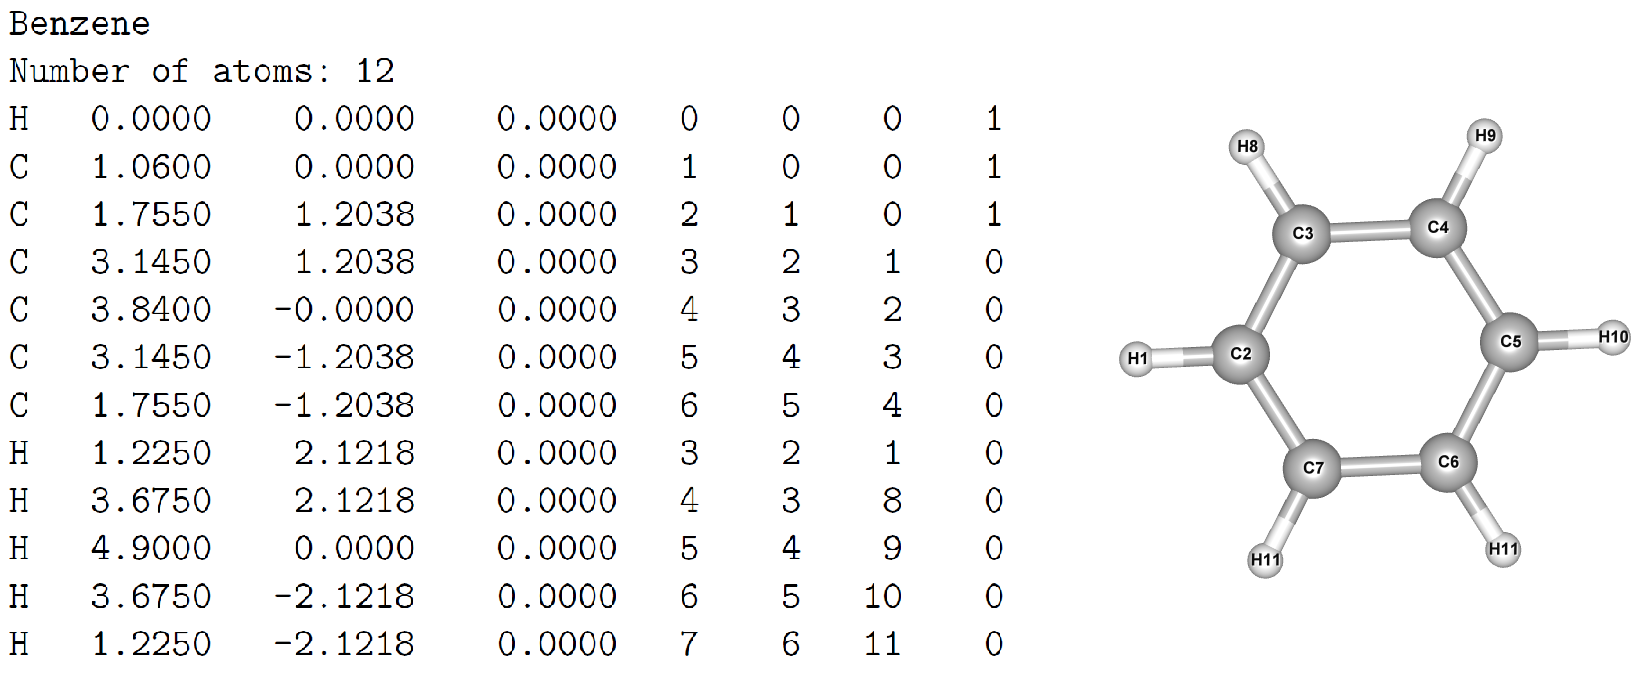
\includegraphics[scale=0.36]{pic/benzene}
\caption{\footnotesize \textbf{Sample of \file{MOL\_1} file and illustration of
the corresponding molecular structure.}}
\label{fig:benzene}
\end{figure}

The 1$^{st}$ atom is H, its coordinates are defined without reference to other
atoms (``0 0 0'').

The 2$^{nd}$ atom is C, its coordinates (in molecular coordinate frame) in
\file{Z\_matrix} will be set only by its distance from the 1$^{st}$ atom
(\emph{i.e.} H described above), but no angles --- (``1 0 0'').

The 3$^{rd}$ atom is C, its coordinates will be set by its distance from the
2$^{nd}$ atom, and the bond angle 3-2-1, but not by torsion angle --- hence we
use ``2 1 0''.

The 4$^{th}$ atom is C, its coordinates will be set by its distance from the
3$^{rd}$ atom, bond angle 4-3-2, and torsion angle 4-3-2-1 --- hence, we use
``3 2 1'' and so forth\ldots until we reach the final, 12$^{th}$ atom, which is
H, defined by its distance from the 7$^{th}$ atom (C), bond angle 12-7-6 and
torsion angle 12-7-6-11 --- hence ``7-6-11''.

The final column is the flexibility flag for the torsion angle. For example, in
C4, the tosion angle is defined by 4-3-2-1. Ideally, this flag should be 1 for
the first three atoms, and 0 --- for the others. If any other flexible torsion
angle exists, specify 1 for this column.


\subsubsection{Polymeric Crystals, \keyword{calculationType}=110 (``linear
chain model'')}

For polymers, the \file{MOL\_1} file is used to represent the geometry of a
monomeric unit, in the same style as for molecular crystals, except that we use
the last column to specify the reactive atoms as shown in the \file{MOL\_1} file
for PVDF:

\begin{figure}[htbp] \centering 
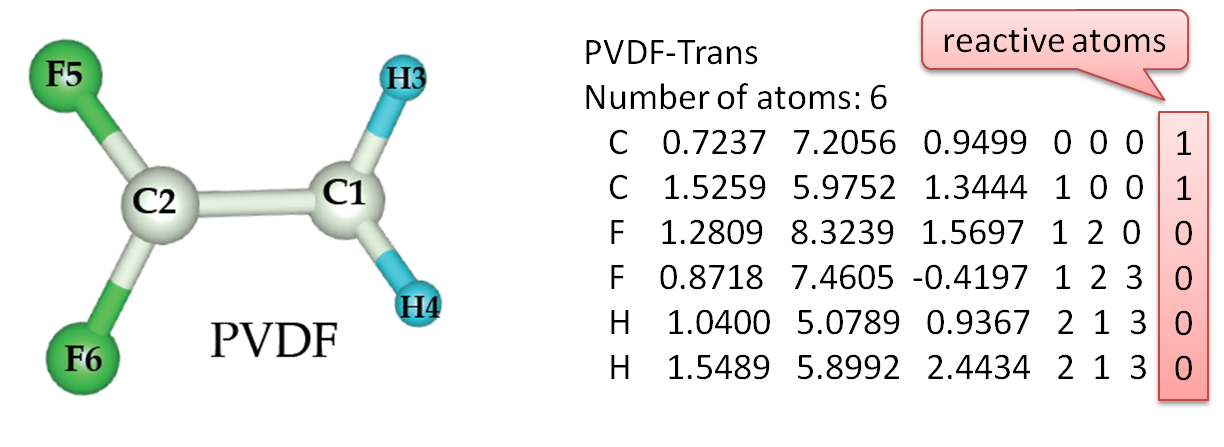
\includegraphics[scale=0.72]{pic/PVDF_MOL}
\caption{\footnotesize \textbf{Sample of \file{MOL\_1} file of PVDF and
illustration of the corresponding monomeric structure.}}
\label{fig:pvdf}
\end{figure}


\subsubsection{Additional inputs for classical forcefields}

The above \file{MOL\_1} files can be used for general cases in USPEX. However,
some classical forcefield based codes need additional information. For instance,
GULP needs to specify the chemical labels and charge. The \file{MOL\_1} file for
aspirin can be written in the following way:
\begin{verbatim}
Aspirin_charge
Number of atoms: 21
H_1     0.2310     3.5173     4.8778     0  0  0   1     0.412884
O_R     0.7821     4.3219     4.9649     1  0  0   1    -0.676228
C_R     0.4427     5.0883     6.0081     2  1  0   1     0.558537
O_2    -0.5272     4.5691     6.6020     3  2  1   0    -0.658770
C_R     1.0228     6.3146     6.3896     3  2  4   0     0.116677
C_R     2.1330     6.8588     5.6931     5  3  2   0     0.311483
C_R     0.4810     7.0546     7.4740     5  3  6   0    -0.119320
O_R     2.8023     6.2292     4.6938     6  5  3   0    -0.574557
C_R     2.6211     8.1356     6.0277     6  5  8   0    -0.083091
C_R     0.9966     8.3146     7.8237     7  5  3   0    -0.103442
H_2    -0.3083     6.6848     8.0128     7  5 10   0     0.198534
C_R     3.6352     5.1872     4.9079     8  6  5   0     0.609295
C_R     2.0623     8.8613     7.0940     9  6  5   0    -0.119297
H_2     3.3963     8.5283     5.4906     9  6 13   0     0.174332
H_2     0.5866     8.8412     8.6013    10  7 13   0     0.205960
O_2     3.9094     4.7941     6.0632    12  8  6   0    -0.588433
C_3     4.2281     4.5327     3.7638    12  8 16   0    -0.271542
H_2     2.4227     9.7890     7.3367    13  9 10   0     0.196738
H_2     3.4269     4.1906     3.1183    17 12  8   0     0.151315
H_2     4.8283     3.6848     4.0792    17 12 19   0     0.131198
H_2     4.8498     5.2464     3.2337    17 12 19   0     0.127726
\end{verbatim}
Here, the keyword \keyword{charge} in the title tells the program to read the 
charge in the additional (last) column.

To work with Tinker, the additional column is used to specify the atomic label
as follows:
\begin{verbatim}
Urea
Number of atoms: 8
C     0.000000    0.000000    0.000000   0 0 0 1  189  
O     0.000000    0.000000    1.214915   1 0 0 1  190  
N     1.137403    0.000000   -0.685090   1 2 0 1  191  
N    -1.137403    0.000000   -0.685090   1 2 3 0  191  
H     1.194247    0.000000   -1.683663   4 1 3 0  192  
H    -1.194247    0.000000   -1.683663   4 1 3 0  192  
H     1.998063    0.000000   -0.138116   2 1 3 0  192  
H    -1.998063    0.000000   -0.138116   2 1 3 0  192  
\end{verbatim}


\subsubsection{How to prepare the \file{MOL} files}

There are plenty of programs which can generate Zmatrix style files, such as
Molden, Avogadro, and so on. The experienced users might have their own way to
prepare these files. For the users' convenience, we have created an online
utility to allow one to generate the USPEX-style \file{MOL} file just from a
file in XYZ format. Please try this utility at
\textcolor{blue}{\url{http://han.ess.sunysb.edu/zmatrix}}.


\subsection{Surfaces} \label{surfaces}
To perform a prediction of surface reconstructions, you have to:
\begin{itemize}
\item Specify \texttt{200} or \texttt{201 : calculationType}.
\item Provide a file containing substrate in VASP5 POSCAR format, as shown
on Fig.~\ref{fig:surface}.
\item Specify the following parameters:
\end{itemize}

\begin{figure}[hbtp]
\centering
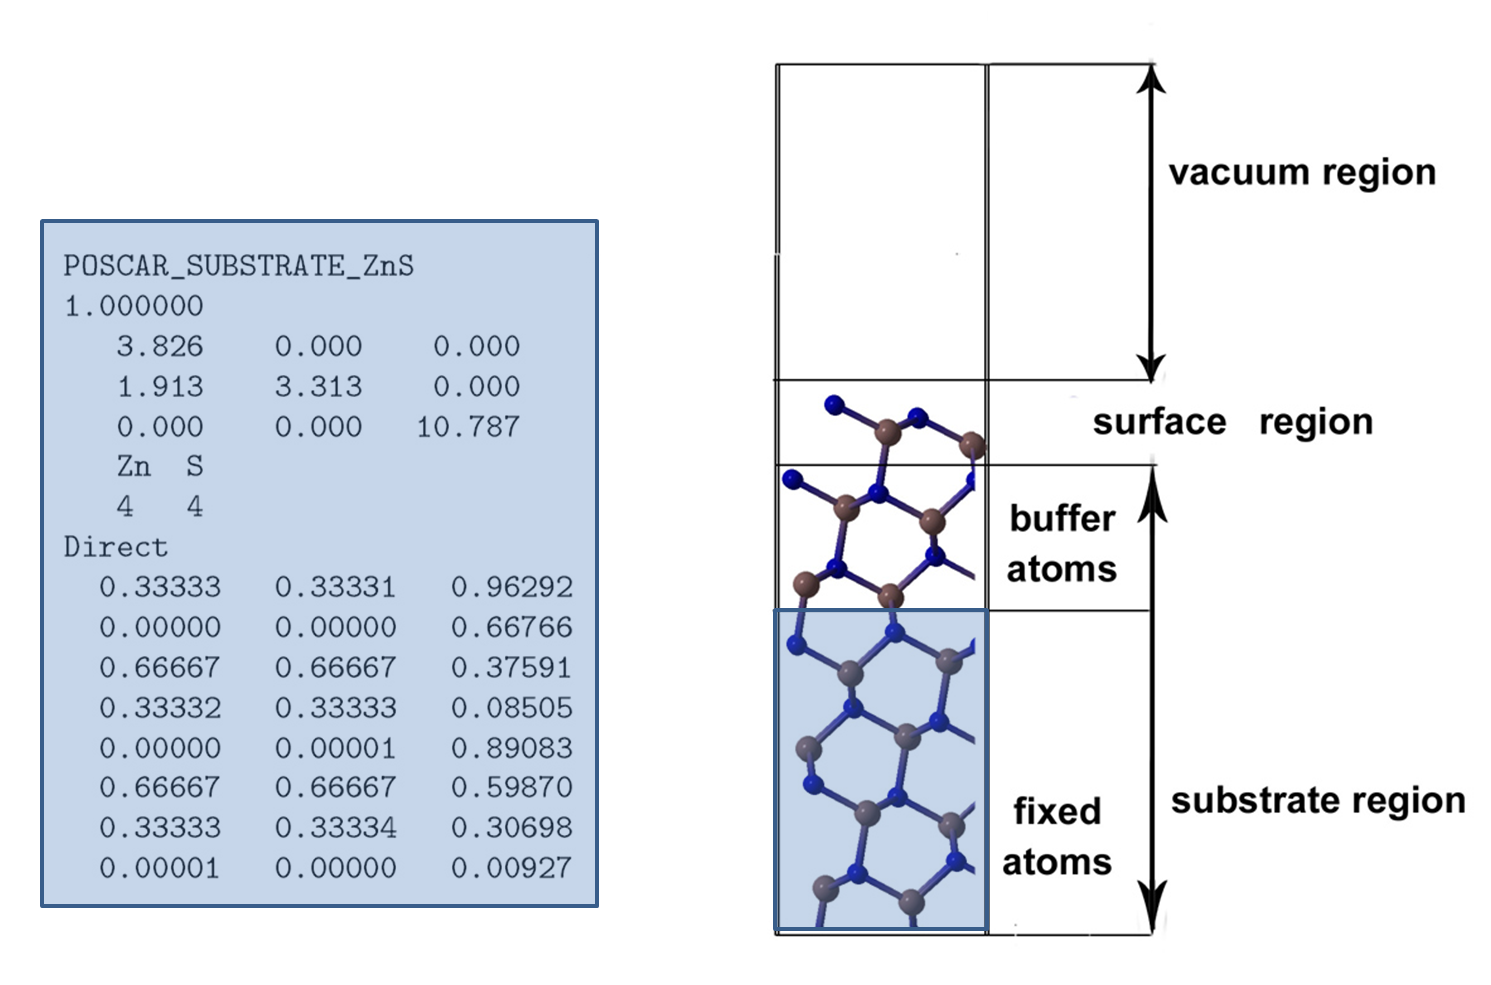
\includegraphics[scale=0.5]{pic/Surface.png}
\caption{\footnotesize \textbf{The surface model used in USPEX.} Note that
\file{POSCAR\_SUBSTRATE} shall exactly represent the geometrical information of
its bulk crystal without vacuum. If the input has large vacuum region, the
program will automatically delete it and provide a new file called
\file{POSCAR\_SUBSTRATE\_NEW}, and this file has to be used in the calculation
(renamed as \file{POSCAR\_SUBSTRATE}).}
\label{fig:surface}
\end{figure}

\begin{verbatim}
% symmetries
2-17
% endSymmetries
\end{verbatim}

\textbf{Note:} If the \keyword{symmetries} tag is present, USPEX will try to
generate structures using plane groups.

\paramacro{thicknessS}{Thickness of surface region. Adatoms are allowed only in
this region.}{}{2.0 \rm $\text{\r{A}}$}{3.5 : thicknessS}{}

\paramacro{thicknessB}{Thickness of buffer region in substrate. This region is
part of \file{POSCAR\_SUBSTRATE}, allowed to relax.}{}{3.0 \rm
$\text{\r{A}}$}{3.0 : thicknessB}{}

\paramacro{reconstruct}{Maximum multiplications of the surface cell, to allow
for complex reconstructions.}{}{1}{1 : reconstruct}{}

\vspace{0.5 cm}

USPEX also provides the possibility of studying the stable configurations with
variable number of surface atoms (to be released in USPEX~10.1). In this case,
stable surface reconstructions are dictated by chemical potentials
\cite{Zhu2013}. A typical set of input is the following:

\begin{verbatim}
******************************************
*      TYPE OF RUN AND SYSTEM            *
******************************************
USPEX  : calculationMethod (USPEX, VCNEB, META)
201    : calculationType (dimension: 0-3; molecule: 0/1; varcomp: 0/1)

% atomType
Si O
% EndAtomType

% numSpecies
2 4
% EndNumSpecies
\end{verbatim}

Here we specify the maximum number of surface atoms in a $1 \times 1$ cell.

\begin{verbatim}
******************************************
*               SURFACES                 *
******************************************
% symmetries
2-17
% endSymmetries

% StoichiometryStart
1 2
% StoichiometryEnd
\end{verbatim}

This defines the stoichiometry of the bulk.

\begin{verbatim}
-23.7563 : E_AB (DFT energy of AmBn compound, in eV per formula unit)
-5.4254  : Mu_A (DFT energy of elemental A, in eV/atom)
-4.9300  : Mu_B (DFT energy of elemental B, in eV/atom)

3.5      : thicknessS (thickness of surface region, 2 A by default )
3.0      : thicknessB (thickness of buffer region in substrate, 3 A by default)
4        : reconstruct (maximum multiplications of cell)
\end{verbatim}

At the moment, USPEX supports variable-composition calculation for the following
cases of surfaces:
\begin{itemize}
\item Reconstructions of elemental surfaces (such as C@diamond(100) surface).
\item Reconstructions of surfaces at binary compounds (such as GaN(0001)
surface).
\item Reconstructions involving foreign species on elemental surfaces (such as
PdO@Pd(100) surface).
\end{itemize}


\subsection{Variable-composition code}

To switch on the variable-composition mode, you have to:
\begin{enumerate}
\item Specify \texttt{301} or \texttt{311} or \texttt{201  : calculationType}.
\item Specify compositional building blocks in \keyword{numSpecies} (see the
description of \keyword{numSpecies} variable).
\item Optionally specify the approximate atomic volumes for each atom type (or
for each compositional block) using keyblock \keyword{Latticevalues}.
\item Specify the following \textit{varcomp-only} options:
\end{enumerate}


\paramacro{firstGeneMax}{How many different compositions are sampled in the
first generation. If 0, then the number is equal to \keyword{initialPopSize}/4.
For binaries, we recommend \keyword{firstGeneMax}=11, for ternaries a higher
value is needed, \emph{e.g.} 30.}{}{11}{10 : firstGeneMax}{}

% PPPPPPPPPPPPPPPPPPPPPPPPP
\paramacro{minAt}{Minimum number of atoms (for
\keyword{calculationType}=301/201/300) or molecules (for
\keyword{calculationType}=311) in the unit cell for the first generation.}{}{No
default}{10  : minAt}{}
 
% PPPPPPPPPPPPPPPPPPPPPPPPP
\paramacro{maxAt}{Maximum number of atoms (for
\keyword{calculationType}=301/201/300 or in META calculations) or molecules (for
\keyword{calculationType}=311) in the unit cell for the first generation.}{}{No
default}{20  : maxAt}{}

% PPPPPPPPPPPPPPPPPPPPPPPPP
\paramacro{fracTrans}{Percentage of structures obtained by transmutation. In
this operator, a randomly selected atom is transmuted into another chemical
species present in the system --- the new chemical identity is chosen randomly
by default, or you can specify it in the block \keyword{specificTrans}, just
like with specific permutation swaps.}{ }{0.1}{0.1   : fracTrans}{}

% PPPPPPPPPPPPPPPPPPPPPPPPP
\paramacro{howManyTrans}{Maximum percentage of atoms in the structure that are
being transmuted (0.1 = 10\%). The fraction of atoms that will be transmuted is
drawn randomly from a homogeneous distribution bounded between 0 and the
fractional parameter \keyword{howManyTrans}.}{}{0.2}{0.2  : howManyTrans}{}

% PPPPPPPPPPPPPPPPPPPPPPPPP
\paramacro{specificTrans}{Specifies allowed transmutations.}{}{\rm blank
line (no specific transmutations)}{\% specificTrans \\
1 2 \\
\% EndTransSpecific}{\textbf{Note:} In this case, atoms of type 1 could be
transmuted into atoms of type 2 and vice versa. If you want to try all possible
transmutations, just leave a blank line inside this keyblock.}

\vspace{0.5cm}

In the case of variable-composition runs, parameter \keyword{keepBestHM} takes a
new meaning --- all structures on the convex hull (\emph{i.e.},
thermodynamically stable states of the multicomponent system) survive, along
with a few metastable states closest to the convex hull --- the total number is
\keyword{keepBestHM}.

For variable-composition runs, it is particularly important to set up the first
generation wisely. Choose a suitably large initial generation size
\keyword{initialPopSize}. Choose a reasonably large number of different
compositions \keyword{firstGeneMax} to be sampled in the first generation (but
not too large --- each composition needs to be sampled several times at least).
Finally, \keyword{minAt} and \keyword{maxAt} should not differ by more than 2
times, and you may need a few calculations with different system sizes:
\emph{e.g.}, 4--8, 8--16, 16--30 atoms, \emph{etc.}

\begin{figure}[htbp] \centering 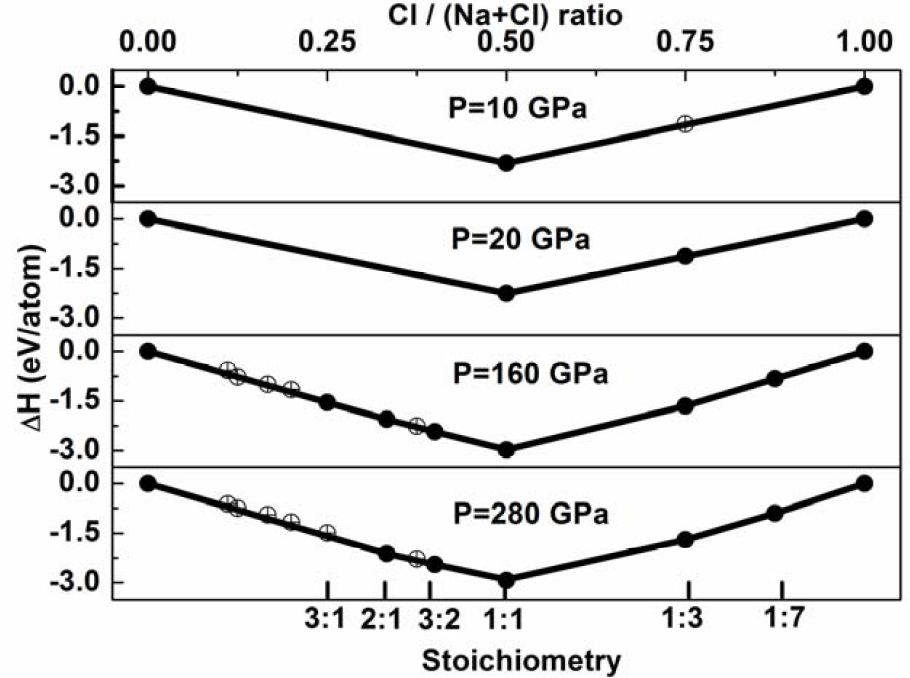
\includegraphics[scale=0.4]{pic/NaCl}
\caption{\footnotesize \textbf{Convex hull diagram for Na-Cl system at selected
pressures.} Solid circles represent stable compounds; open circles ---
metastable compounds.}
\label{fig:NaCl}
\end{figure}

An additional comment for VASP users --- if you want to perform a
variable-composition run, let's say for the Na-Cl system, you should make sure
the atomic types are given correctly in \file{INPUT.txt}, and put
pseudopotential files \file{POTCAR\_Na} and \file{POTCAR\_Cl} in the folder
\file{$\sim$/StructurePrediction/Specific/}. USPEX will then recognize each atom
and take each atom's \file{POTCAR} file appropriately for the calculations.
Fig.~\ref{fig:NaCl} shows thermodynamics of stable sodium chlorides discovered
using USPEX and confirmed by experiment \cite{Zhang2013}.


\subsection{Evolutionary metadynamics code} \label{metadynamics}

This is a very powerful method for finding the global minimum, as well as many
low-energy metastable structures that are potentially kinetically accessible
from the starting structure. The starting structure has to be high-quality and
is given in the file \file{POSCAR\_1}.

Evolutionary metadynamics is only enabled with the VASP and GULP codes at the
moment.

To switch on the evolutionary metadynamics mode, you have to:

\begin{enumerate}
\item Specify

\texttt{META  : calculationMethod}

\texttt{300   : calculationType}

\item Create file \file{POSCAR\_1} in the VASP5 format in your folder
(evolutionary metadynamics requires a good starting structure, relaxed at the
pressure of interest).

\item Specify the population size (in this case, this is the number of
softmutations at each metastep):

\texttt{30    : populationSize}

\item Specify the pressure:

%PPPPPPPPPPPPPPPPPPPPPPPPP
\paramacro{ExternalPressure}{The pressure at which you want to perform the
calculation, in GPa.}{}{\rm no default}{10  : ExternalPressure (GPa)}{}

\item Specify the following metadynamics-only options:
\end{enumerate}

% PPPPPPPPPPPPPPPPPPPPPPPPP
\paramacro{GaussianWidth}{The width of each of the Gaussians added to the energy
surface to accelerate phase transitions. A good rule of thumb is to choose a
value close to 0.10--0.15$L$, where $L$ is the minimum length of the unit cell,
in Angstroms.}{}{$0.10 \times L$ \rm ($\text{\r{A}}$)}{0.80  : GaussianWidth}{}

% PPPPPPPPPPPPPPPPPPPPPPPPP
\paramacro{GaussianHeight}{The height of each of the Gaussians added to the
energy surface to accelerate phase transitions. A good rule of thumb
(Marto\v{n}\'{a}k \emph{et al.}, 2005) is to choose a value close to $L(\delta
h)^2 G$, where $L$ is the average length of the unit cell in Angstroms, $\delta
h$ is the Gaussian width in Angstroms (see below), and $G$ is the shear modulus
in kbars.}{}{$1000 \times (0.10 \times L)^2 \times L = 10 \times L^3$ \rm
($\text{\r{A}}^3$kbar)}{2000 : GaussianHeight}{}

% PPPPPPPPPPPPPPPPPPPPPPPPP
\paramacro{FullRelax}{Metadynamics as such only relaxes structures within a
fixed cell. For analysis, you need to perform complete structure relaxation
(\emph{i.e.} relaxing also the cell).}{
\begin{itemize}
  \item \keyword{FullRelax}=0 --- no full relaxation will be performed
  (very fast option, but inconvenient for analysis of the results).
  
  \item \keyword{FullRelax}=1 --- only the best structure of the generation
  will be fully relaxed (also fast, sometimes sufficient).
  
  \item \keyword{FullRelax}=2 --- all inequivalent structures are fully relaxed
  (still fast, only $\sim$2 times slower than \keyword{FullRelax}=1, but
  provides a lot more insight. Strongly recommended for most cases).
\end{itemize}
}{2}{2 : FullRelax }{}

\vspace{0.5 cm}
For full relaxation, when performing evolutionary metadynamics the
format of the block \keyword{abinitioCode} is slightly different, for example:
\begin{verbatim}
    abinitioCode
    3 3 3 3 (3 3)
    ENDabinit
\end{verbatim}

In the example above, there are four stages of relaxation within a fixed cell,
and two stages of full relaxation (in parentheses). Remember that in the last
fixed-cell stage of relaxation, pressure tensor must be accurate --- this is
what drives metadynamics. Only VASP, SIESTA, and GULP codes are supported at the
moment.

%\paramacro{maxCellIncrease}{Maximum cell multiplication factor when supercell is
%built.}{}{5}{4 : maxCellIncrease}{}

\paramacro{maxVectorLength}{Together with \keyword{minVectorLength} the boundary
values for basic cell lengths in evolutionary metadynamics (note that this is a
different meaning for \keyword{minVectorLength} from normal calculations, and
\keyword{maxVectorLength} is only used in evolutionary metadynamics). When any
of the basic cell lengths becomes smaller than \keyword{minVectorLength} or
larger than \keyword{maxVectorLength}, we add a steep correction ``force'' in
metadynamics, which drives cell evolution towards ``good'' values. The
correction forces are exactly zero when all basic cell lengths are in the
``good'' range.}{}{No default}{12.0 : minVectorLength}{}

%\paramacro{maxModesPerVectorPerAtom}{Limits the number of modes per
%k-vector (not found in USPEX SVN!).}{}{}{}{}

\vspace{0.5cm}

\begin{figure}[htbp] \centering
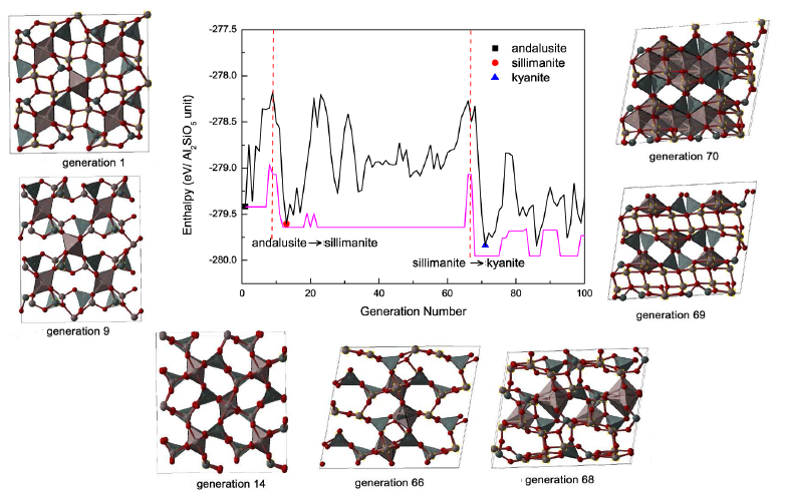
\includegraphics[scale=0.8]{pic/evolutionary_metadynamics}
\caption{\footnotesize \textbf{Enthalpy evolution during the compression on
andalusite (Al$_2$SiO$_5$) at 10 GPa (black line: enthalpies for best structures
with constant h; magenta line: enthalpies for best structures after full
relaxation).} Sequence of structures obtained in this run: generation 1
(andalusite) $\rightarrow$ generation 9 (sillimanite) $\rightarrow$ generation
14 $\rightarrow$ generation 66 $\rightarrow$ generation 68 $\rightarrow$
generation 69 $\rightarrow$ generation 70 (kyanite).}
\label{fig:evolutionary_metadynamics}
\end{figure}

When you run metadynamics, additional files will be found in the \file{results1}
folder, most importantly:

\begin{itemize}
  \item \file{force.dat} --- analysis of forces on the cell, internal
  (\keyword{f\_c}) and from the Gaussians (\keyword{f\_g});
  \item \file{presten} --- pressure tensor;
  \item \file{lattice.dat}  --- cell shape change during the simulation;
  \item \file{enthalpies} and \file{enthalpies\_relaxed} --- enthalpies of
  structures at each metastep at fixed cell and after full relaxation,
  respectively;
  \item \file{gatheredPOSCARS} and \file{gatheredPOSCARS\_relaxed} ---
  structures at fixed cell and after full relaxation, respectively.
\end{itemize}

Fig.~\ref{fig:evolutionary_metadynamics} shows an example of use of evolutionary
metadynamics: starting from one Al$_2$SiO$_5$ polymorph (andalusite), we
obtained the other two known polymorphs (kyanite and sillimanite) and
non-trivial phase transformation mechanisms.


\subsection{Particle swarm optimization (PSO) code} \label{pso}

In the field of crystal and cluster structure prediction, several approaches
proved to be successful for small systems. Particle Swarm Optimization (PSO),
pioneered in this field by Boldyrev \cite{Boldyrev2007}, is a special class of
evolutionary algorithms where a population (swarm) of candidate solutions
(called ``particles'') is moved in the search space according to a few simple
formulae. The movements of the particles are guided by their own best known
position in the search space as well as the entire swarm's best known position.
Initially, the coordinates $\chi$ and 'velocities' $\upsilon$ of the particles
are generated randomly. Then at every step, the positions and velocities are
updated according to the formulae:

\begin{equation}\label{eq:pso}
\begin{aligned}
\upsilon'_{i} &= \omega \cdot \upsilon_{i} + \varphi_{p} \cdot r_{p} \cdot
(p_{i} - \chi_{i}) + \varphi_{g} \cdot r_{g} \cdot (g - \chi_{i}),\\
\chi'_{i} &= \chi_{i} + \upsilon'_{i}.
\end{aligned}
\end{equation}

Here $\omega$, $\varphi_{p}$ and $\varphi_{g}$ are weight factors that control
the behavior and efficiency of the PSO algorithm; $r_{p}$ and $r_{g}$ are random
numbers in the [0; 1] range generated separately for every particle at every
step; $p_{i}$ is the best known position of particle $i$ and $g$ is the best
known position of the entire swarm.

Such an algorithm, despite its simplicity, can work \cite{Boldyrev2007}. Key
points to improve with respect to previous implementations \cite{Boldyrev2007,
Wang2010} are (1) metric of the search space (it is not trivial to map crystal
structures uniquely onto a coordinate system) and (2) ways to evolve structures
in PSO, \emph{i.e.} variation operators.

\begin{figure}[htbp] \centering
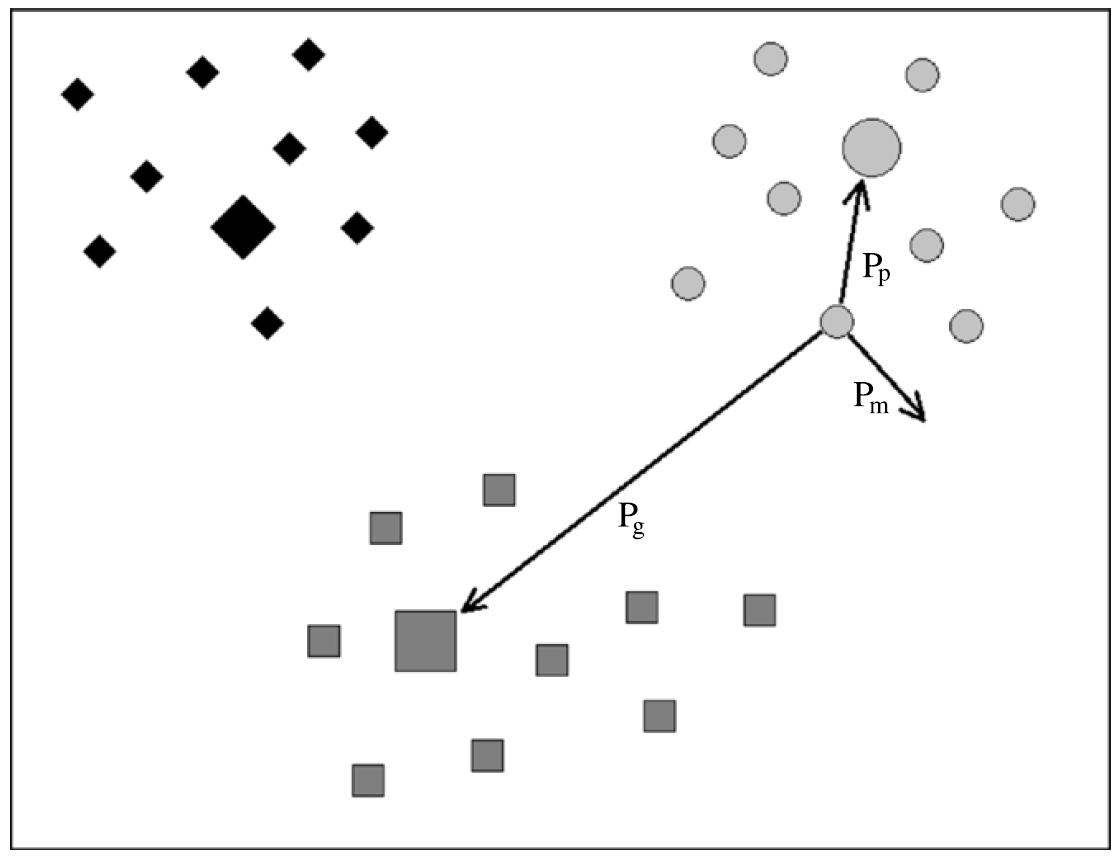
\includegraphics[scale=0.3]{pic/PSO}
\caption{\footnotesize \textbf{Illustration of PSO-USPEX hybrid algorithm for
the population of three individuals (marked by diamonds, squares and circles)
after 10 generations.} Best position for each particle is marked by an enlarged
symbol. The best structure is the big square. The structure shown by circle can
be either mutated, create a child with its historically best position (large
circle) or the best position of entire population (large square) using heredity
operator with probabilities $P_{m}$, $P_{p}$ and $P_{g}$, respectively.}
\label{fig:pso}
\end{figure}

Evolving the particles by determining the speed $\upsilon_{i}$ (\ref{eq:pso})
directly from coordinates of the atoms and cell parameters of two structures (as
in Ref. \cite{Wang2010}) cannot be productive. Our solution is to use
fingerprint distances \cite{Oganov2009} as the most natural metric for the
energy landscape, and variation operators of USPEX for evolving the 'PSO
particles' (\emph{i.e.} structures) as the most efficient unbiased ways to
evolve a population of structures. Namely, the particle is either mutated (to
imitate a random move), or participates in heredity with its best known position
or in heredity with the best known population position (to imitate PSO moves in
the direction of these positions). Instead of applying at each step all moves
with some weights (see Eq.~\ref{eq:pso}), we apply them one at a time with
probabilities described by formulae:

\begin{equation}\label{eq:pso2}
\begin{aligned}
P_{m} = \frac{\omega}{\Sigma};\qquad
&P_{p} = \frac{\varphi_{p} \cdot r_{p} \cdot D_{p}}{\Sigma};\qquad
P_{g} = \frac{\varphi_{g} \cdot r_{g} \cdot D_{g}}{\Sigma};\\
&\Sigma = \omega + \varphi_{p} \cdot r_{p} \cdot D_{p} + \varphi_{g} \cdot
r_{g} \cdot D_{g},
\end{aligned}
\end{equation}

where $D_{p}$ is a fingerprint distance between current and best position of a
particle, while $D_{g}$ is a fingerprint distance between the current position
of the particle and best known position of the entire population. Our tests,
performed on a few diverse systems, show that this approach (which we call
``cor-PSO'', \emph{i.e.} corrected PSO) is relatively successful and works
better than previous versions of PSO, but still cannot compete with the USPEX
algorithm \cite{Oganov2006, Lyakhov2010} for success rate or efficiency.

The following variables are unique for \keyword{calculationMethod}=PSO:

\paramacro{PSO\_softMut}{Weight of softmutation ($\omega$ in
eq.~\ref{eq:pso2}).}{}{1}{1 : PSO\_softMut}{}

\paramacro{PSO\_BestStruc}{Weight of heredity with the best position of the same
PSO particle ($\varphi_{p}$ in eq.~\ref{eq:pso2}).}{}{1}{1 : PSO\_BestStruc}{}

\paramacro{PSO\_BestEver}{Weight of heredity with the globally best PSO particle
($\varphi_{g}$ in eq.~\ref{eq:pso2}).}{}{1}{1 : PSO\_BestEver}{}


%%%%%%%%%%%%%%%%%%%%%%%%%%%%%%%%%%%%%%%%%%%%%%%%%%%%%%%%%%%%%%%%%%%%%%%%%%%%%%%%
\newpage
\section{Prediction of Phase Transition Pathways}

Phase transitions determine many aspects of the behavior of materials. Thus, it
is essential to reveal possible mechanisms of structural phase transitions.


\subsection{Variable-Cell Nudged-Elastic-Band (VCNEB) method} \label{vcneb}

Prediction of a phase transition mechanism can be considered as a double-ended
problem, in which the algorithm has to locate the intermediate states. The
nudged elastic band (NEB) \cite{Mills1995, Henkelman2000a, Henkelman2000b}
method is a widely used technique for solving double-ended problems, an
efficient and robust approach for seeking the reaction paths and the saddle
points along the ``minimum energy path'' (MEP) on the potential energy surface
between the two endpoints. The NEB method has been successfully applied to
molecular chemical reactions, surfaces, and defect migration, in particular it
could provide the energy barrier between the given initial and final states of a
phase transition process. Unfortunately, most of the problems treated by the NEB
method are considered under the constraint of constant unit cell --- which
precludes it from being used for phase transitions (which involve the variation
of the unit cell along the transition path).

\begin{figure}[htbp] \centering
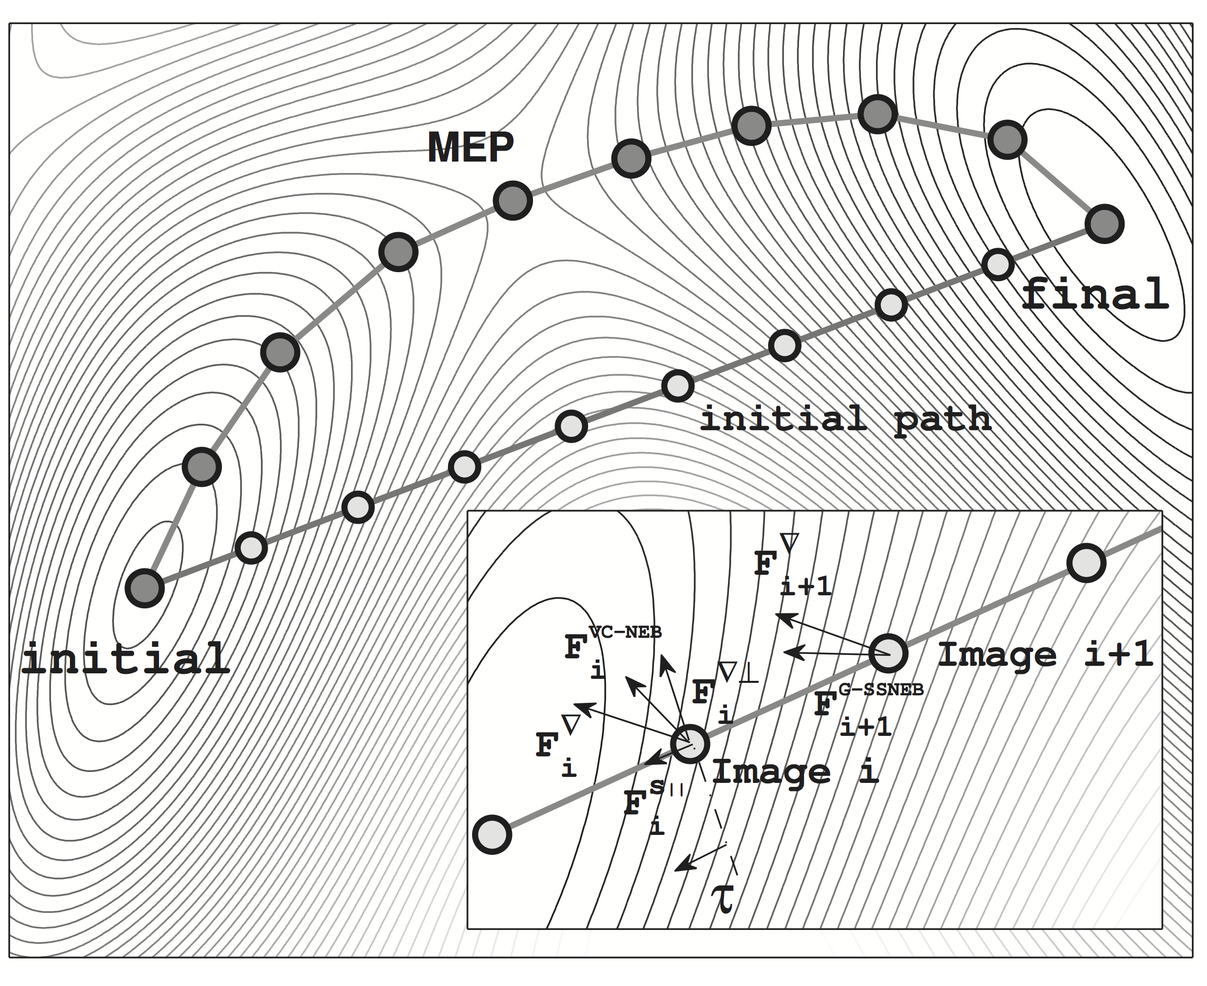
\includegraphics[scale=0.95]{pic/VCNEB}
\caption{\footnotesize \textbf{The minimum energy path (line with gray circles)
and initial path on a model 2D enthalpy surface.} {The forces in the VC-NEB
method on Image $i$ are shown in the inset. $\mathbf{F}^{\nabla}_{i}$ is the
potential force in the gradient direction. $\mathbf{F}^{\nabla\bot}_{i}$ and
$\mathbf{F}^{s\parallel}_{i}$ are the transverse component of
$\mathbf{F}^{\nabla}_{i}$ and the spring force, respectively.}}
\label{fig:VCNEB}
\end{figure}

The variable cell NEB (VC-NEB) method \cite{Qian2013}, which we have developed
with somewhat different formulation, treats the cell and atomic coordinates on
an equal footing and operates in an expanded configuration space under the
condition of constant pressure. Our VC-NEB method within the first principles
framework has been added to USPEX code as a new part. The VC-NEB method is a
more general tool for exploring the activation paths between the two endpoints
of a phase transition process within a larger configuration space. Every
structure on the pathway in the VCNEB method is regarded as an ``Image''.


\subsection{Input options for VCNEB}

The VCNEB method is only enabled with the VASP, GULP and Quantum Espresso codes
at the moment.

To switch on the VCNEB mode, you have to:

\begin{enumerate}
  \item Specify

  \texttt{VCNEB  : calculationMethod}
  
  \item Create a file \file{Images} in the VASP4 format in your folder (VCNEB
  requires at least two structures, initial and final phases, to run the phase
  transition pathway prediction).
  
  \item Specify the following VCNEB options:
\end{enumerate}

%PPPPPPPPPPPPPPPPPPPPPPPPP

% PPPPPPPPPPPPPPPPPPPP
\paramacro{vcnebType}{Specifies type of the VCNEB calculation. This variable
consists of three indices: \emph{calculation option}, \emph{Image number
variability}, and \emph{spring constant variability}:
\begin{itemize}
  \item calculation option:
  \begin{itemize}
    \item[] ``1'' --- the VCNEB method;
    \item[] ``2'' --- structure relaxation mode with no VCNEB calculation.
  \end{itemize}
  \item \texttt{Variable-Image-Number} method:
  \begin{itemize}
    \item[] ``0'' ---  the number of Images in VCNEB calculation is fixed;
    \item[] ``1'' ---  the number of Images in VCNEB calculation is variable.
  \end{itemize}
  \item variability of spring constant:
  \begin{itemize}
    \item[] ``0'' --- fixed spring constant;
    \item[] ``1'' --- variable spring constant.
  \end{itemize}
\end{itemize}
}{}{110}{
111    : vcnebType
}{\textbf{Note:} If \keyword{vcnebType}=111, \emph{i.e.}, a calculation for
VCNEB calculation with variable number of Images and variable spring constant is
to be performed. We strongly suggest users to run a variable number of Images in
VCNEB calculations when investigating the reconstructive phase transitions.}

\paramacro{numImages}{Initial number of Images to perform the
calculation.}{}{9}{13  : numImages}{}

\paramacro{numSteps}{Maximum steps of performing the VCNEB calculation.}{}
{200}{500  : numSteps}{\textbf{Notes:} (1) When \keyword{numSteps}=-1, the
initial pathway will only be generated without running energy calculations.
(2) Convergence of VCNEB pathways is usually rather slow. We recommend to set
\keyword{numSteps} to at least 500.}

\paramacro{optReadImages}{Options for reading the \file{Images} file:
\begin{itemize}
  \item ``0'' --- All images (\keyword{numImages}) are needed and specified in
  \file{Images} file;
  \item ``1'' --- Only initial and final images are needed and would be read in
  \file{Images} file;
  \item ``2'' --- The initial, final and any specified intermediate Images will
  be read in \file{Images} file.
\end{itemize}
}{}{2}{1  : optReadImages}
{\textbf{Note:} In all options, the initial and final images must be specified. 
Automatic linear interpolation will be applied to generated the initial Images
in option 1 and 2.}

\paramacro{optimizerType}{Optimization algorithm option of structure relaxation: 
\begin{itemize}
  \item ``1'' --- Steep Descent (SD);
  \item ``2'' --- FIRE (Fast Inertial Relaxation Engine) Algorithm
  \cite{Bitzek2006}.
\end{itemize}
}{}{1 {\rm (SD) --- for VCNEB calculations;} 2 {\rm (FIRE) --- for structure
relaxation}}{1  : optimizerType}{}

\paramacro{optRelaxType}{Structure relaxation mode:
\begin{itemize}
  \item ``1'' --- relax only atomic positions (with cell fixed), \emph{e.g.}
  as in the classical NEB method;
  \item ``2'' --- relax only cell lattice (used only for testing);
  \item ``3'' --- full relaxation of atomic positions and cell lattice.
\end{itemize}
}{}{3}{3  : optRelaxType}{}

\paramacro{dt}{Time step for structure relaxation.}{}{0.05}{0.1  : dt}{}
{\textbf{Note:} If \keyword{dt} is very small, the calculations will be very
slow. If \keyword{dt} is too large, the calculation will be unstable and often 
generate meaningless pathways.}

\paramacro{ConvThreshold}{Halting criteria condition for RMS (Root Mean Square
forces) on images.}{}{0.003~\rm{eV/$\text{\r{A}}$}}{0.005  : ConvThreshold}{}

\paramacro{VarPathLength}{Criterion for path length between Images for variable
Image method. When the length between two neighbor images is larger than 1.5
times of \keyword{VarPathLength}, a new image will be added between the two
images using linear interpolation; when less then 0.5 the value, the second
image will be removed.}{}{\rm The average pathlength between Images of the
initial pathway}{0.3  : VarPathLength}{}

\paramacro{K$\_$min}{Minimum spring constant, only used in variable-spring
constant VCNEB (in eV/$\text{\r{A}}^2$).}{}{5}{3  : K$\_$min}{}

\paramacro{K$\_$max}{Maximum spring constant, only used in variable-spring
constant VCNEB (in eV/$\text{\r{A}}^2$).}{}{5}{6  : K$\_$max}{}

\paramacro{Kconstant}{Spring constant, Only used in fixed-spring constant
VCNEB (in eV/$\text{\r{A}}^2$).}{}{5}{4  : Kconstant}{}

\paramacro{optFreezing}{Option for freezing the Image structure. Image structure
will be frozen when \keyword{ConvThreshold} is achieved if enabled. Image
structure freezing options:
\begin{itemize}
  \item ``0'' --- no Images freeze any time;
  \item ``1'' --- freeze when \keyword{ConvThreshold} is achieved.
\end{itemize}
}
{}{0}{1  : optFreezing}{}

\paramacro{optMethodCIDI}{Option for Climbing-Image (CI) and Downing-Image (DI)
method. This method is only suggested to be used when you have a reasonable and
well converged pathway. CI/DI-Image method options:
\begin{itemize}
  \item ``0''  --- CI/DI method not used;
  \item ``1''  --- single CI method, only the highest energy or user-provided
  transition state (TS) will be used for CI;
  \item ``-1'' --- single DI method, only the lowest energy or user-provided
  local minimum state (LM) will be used for DI;
  \item ``2''  --- mixed multi-CI/DI method, the sequential numbers of TS and
  LM states need to be provided;
\end{itemize}
}
{}{0}{1  : optMethodCIDI}{}

\paramacro{startCIDIStep}{CI/DI method starting step number, only available when
\keyword{optMethodCIDI}=1.} {}{100}{200  : startCIDIStep}{}


\paramacro{pickupImages}{Images ID picked up for CI/DI-Image method. }{}{\rm
Image ID of transition state and  local minimum state Images}{\% pickupImages \\
9 11 17 \\
\% EndPickupImages}{ \textbf{Note:} In this case, the 9$^{th}$, 11$^{th}$ and
17$^{th}$ Images will be picked up for applying CI/DI-Image method. The Image at
transition state will be applied with CI-Image method and the Image at local
minimum state will be applied DI-Image method automatically.}

\paramacro{FormatType}{ The format of structures in pathway output file, locates
at \file{results1/PATH/}. Pathway structures output format:
\begin{itemize}
  \item ``1'' --- XCRYSDEN format (.xsf file);
  \item ``2'' --- VASP POSCAR;
  \item ``3'' --- XYZ format with cell lattice.
\end{itemize}
}
{}{2}{1  : FormatType}{}

\paramacro{PrintStep}{Save the VNCEB restart files locating at
\file{results1/STEP/} every \keyword{PrintStep} steps.}{}{1}{10  : PrintStep}
{\textbf{Note:} For empirical code, such as GULP, we suggest users to set
\keyword{PrintStep}=10 to reduce time cost of saving the restart files.}

\begin{figure}[htbp] \centering
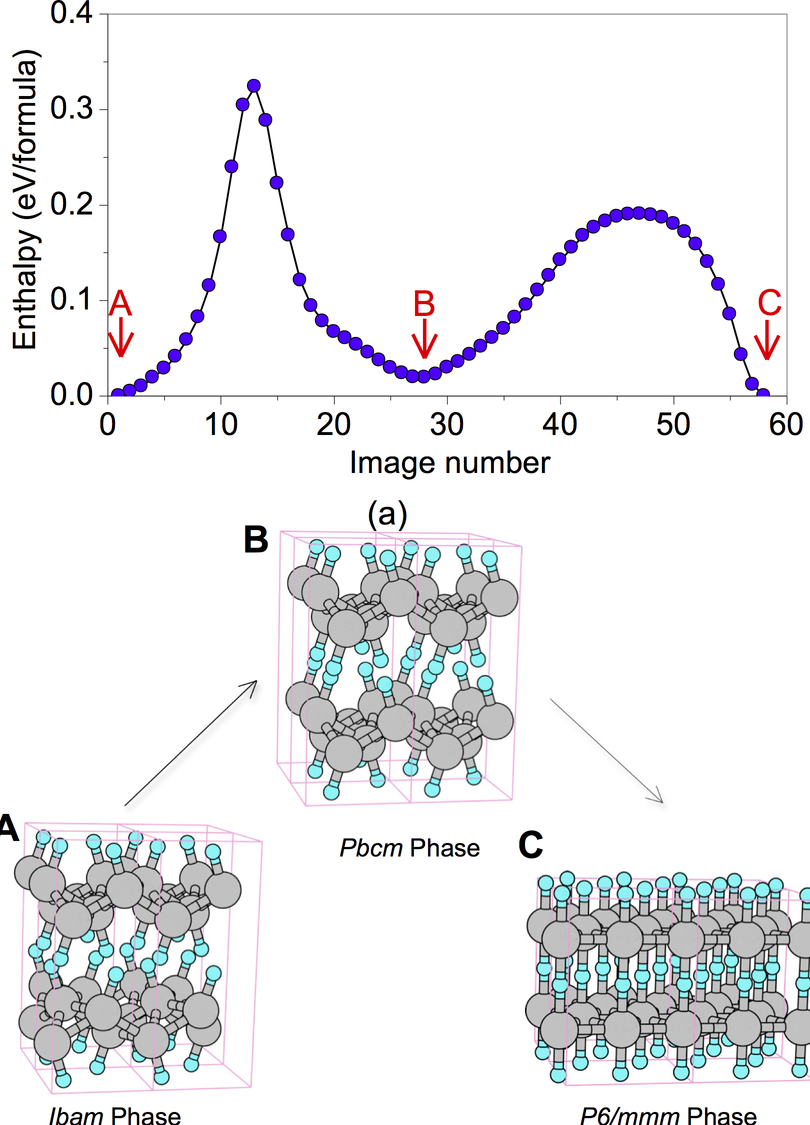
\includegraphics[scale=1.3]{pic/VCNEB_BH}
\caption{\footnotesize \textbf{The $Ibam$$\rightarrow$$P6/mmm$ transition of BH
at 168~GPa \cite{Qian2013}}. A $Pbcm$ intermediate phase is revealed. The saddle
points on $Ibam$$\rightarrow$$Pbcm$ and $Pbcm$$\rightarrow$$P6/mmm$ segments
have barriers of 0.32 and 0.19~eV/f.u., respectively.}
\label{fig:VCNEB_BH}
\end{figure}

\vspace{1.0cm}

Fig.~\ref{fig:VCNEB_BH} shows an example of use of the VCNEB method: phase
transition mechanism and energy barrier starting from the
$Ibam$$\rightarrow$$P6/mmm$ transition of BH system at 168~GPa, we obtained a
$Pbcm$ intermediate phase.

\newpage
\subsection{How to set the initial pathway in the VC-NEB calculation}

The VC-NEB method is very efficient for finding the phase transition path, but
we must also carefully prepare the initial path. The cell rotations happen near
the initial and final structures during the VC-NEB calculation, where the
pathway includes a lot of  identical structures near the initial and finial
images. To remove these useless rotations, our improved
\texttt{Variable-Image-Number} method will prevent cell rotations automatically,
which saves quite a lot of time.

Alternatively, you can apply the rotation-avoiding technique before you apply
the VC-NEB method when generating the initial image set. The general $3 \times
3$ rotation matrix with Euler angles $R(\phi, \theta, \psi)$ and the lattice
mirror operator $M(x, y, z)$ matrix are defined. Before performing a VC-NEB
calculation, the global numerical search in space of Euler angles and mirror
operator are used to find the minimal lattice cell transformation distance
$\Delta h$:

\begin{equation}
\Delta h = \left| {h_{initial} - R(\phi,\theta,\psi) M(x,y,z)h_{final}}\right|.
\end{equation}

The rotation-avoiding lattice vector of the final image $\tilde h_{final}$ is
assigned as the endpoint image:

\begin{equation}
\tilde h_{final} = R(\phi,\theta,\psi)M(x,y,z)h_{final}.
\end{equation}

More important, we need to prevent the arbitrariness assigning the atomic
fractional coordinates $\mathbf{r}_{v}$ of the initial and finial images
(correctly mapping the atoms at the initial and final structures). Otherwise,
the calculation will be hard to converge or several identical paths can be found
in a calculation, as shown in Fig.~\ref{fig:VCNEB_pathway}. For more complicated
systems, you will get some unreasonable or messy pathways if you don't have a
good initial pathway. Global numerical search for minimizing the distance
between the atoms from two endpoint images helps the VC-NEB method to reassign
the atom sequence. The ability to automatically create model paths before the
VC-NEB calculation is crucial for the stability and convergence of the
algorithm, and is a prerequisite for studying large and complex systems.

\begin{figure}[htbp] \centering
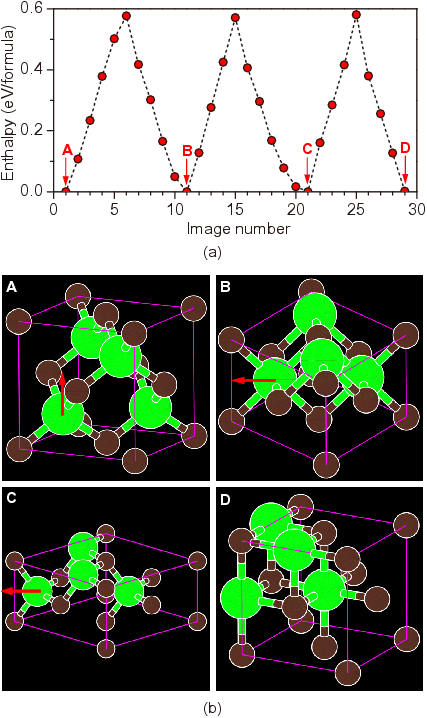
\includegraphics[scale=0.8]{pic/VCNEB_pathway}
\caption{\footnotesize \textbf{Identical pathways found when setting up a
``bad'' initial Image file}. The pathway is for the B3$\rightarrow$B1 phase
transition in GaN at the equilibrium pressure 45.0~GPa. At Images 11 and 21, B1
and B3 structures in a monoclinic cell are found during the MEP searching,
respectively. The Ga atoms move along the arrow directions during the phase
transition.}
\label{fig:VCNEB_pathway}
\end{figure}


%%%%%%%%%%%%%%%%%%%%%%%%%%%%%%%%%%%%%%%%%%%%%%%%%%%%%%%%%%%%%%%%%%%%%%%%%%%%%%%%
\newpage
\section{Online utilities} \label{utilities}
We have created a number of useful online utilities, which can be used for
preparing USPEX input and for post-processing. The utilities are available at:

\begin{center}
\textcolor{blue}{\url{http://han.ess.sunysb.edu}}
\end{center}

Below you can find information about each one of them.

\subsection{Structure characterization}
Here we have 4 utilities:
\begin{itemize}

\item \textcolor{blue}{\href{http://han.ess.sunysb.edu/fingerprints}{Fingerprints}}
--- the utility calculates and plots fingerprint function, which is a crystal
structure descriptor, a 1D-function related to the pair correlation function
and diffraction patterns. It does not depend on absolute atomic coordinates, but
only on interatomic distances. Small deviations in atomic positions will
influence fingerprints only slightly, \emph{i.e.} they are numerically robust.

\item \textcolor{blue}{\href{http://han.ess.sunysb.edu/multifingerprint}{Multifingerprint}}
--- the utility calculates average quasi-entropy, A-order and S-order for a set
of structures. Also it filters unique structures by cosine distances difference
$\geq$~0.003, identifies the symmetry of these structures and lists them in the
\file{uniq\_gatheredPOSCARS} file.

\item \textcolor{blue}{\href{http://han.ess.sunysb.edu/poscar2cif}{POSCAR2CIF}}
--- determines space group and prepares a \file{CIF} file from a \file{POSCAR}
file.

\item \textcolor{blue}{\href{http://han.ess.sunysb.edu/cif2poscar}{CIF2POSCAR}}
--- prepares a \file{POSCAR} file from a \file{CIF} file.

\item \textcolor{blue}{\href{http://han.ess.sunysb.edu/xsf2poscar}{XSF2POSCAR}}
--- prepares a \file{POSCAR} file from a \file{XSF} (XCRYSDEN) file.

\end{itemize}

\subsection{Properties calculation}
Here we have 2 utilities:
\begin{itemize}

\item \textcolor{blue}{\href{http://han.ess.sunysb.edu/hardness}{Hardness}}
--- the utility is to calculate hardness based on the Lyakhov-Oganov model.

\item \textcolor{blue}{\href{http://han.ess.sunysb.edu/EELS}{EELS}}
--- the utility calculates the Electron Energy Loss Spectrum (EELS). Written by
Priya Johari.

\end{itemize}

\subsection{Molecular crystals}
Here we have 2 utilities:
\begin{itemize}

\item \textcolor{blue}{\href{http://han.ess.sunysb.edu/MOL_precheck}{MOL precheck}}
--- the utility allows you to check \file{MOL\_1} files before running USPEX
calculations with \keyword{calculationType}=310/311/110.

\item \textcolor{blue}{\href{http://han.ess.sunysb.edu/zmatrix}{Zmatrix}}
--- the utility converts \file{XYZ} file to USPEX \file{MOL\_1} file.

\end{itemize}

\subsection{Surfaces}
\textcolor{blue}{\href{http://han.ess.sunysb.edu/substrate}{Substrate}} 
--- a program which prepares a substrate from a \file{POSCAR}/\file{CIF} file
and specified Miller indices, thickness of the layer, and shift. The resulting
\file{POSCAR} file can be used for \keyword{calculationType}=200/201 as a
substrate for surface calculations.


\subsection{Miscellaneous}
Here we have the following:
\begin{itemize}

\item \textcolor{blue}{\href{http://han.ess.sunysb.edu/input_generator}{Input generator}}
--- USPEX \file{INPUT.txt} generator. The utility can help beginners to create a
correct input for USPEX calculations.

\item \textcolor{blue}{\href{http://han.ess.sunysb.edu/volume_estimation}{Volume estimation}}
---  the utility estimates volumes of non-molecular and molecular crystals for
USPEX (for \file{INPUT.txt} file). 

\item \textcolor{blue}{\href{http://han.ess.sunysb.edu/uspex_manual}{USPEX manual}}
--- online version of this manual.

\item \textcolor{blue}{\href{http://han.ess.sunysb.edu/uspex_examples}{USPEX examples}}
--- archives with USPEX examples for versions 9.3.9 and 9.4.2.

\end{itemize}


%%%%%%%%%%%%%%%%%%%%%%%%%%%%%%%%%%%%%%%%%%%%%%%%%%%%%%%%%%%%%%%%%%%%%%%%%%%%%%%%
\newpage
\section{Frequently Asked Questions}

\subsection{How can I visualize the results?} \label{faq_visualization}
USPEX produces a large set of numbers (structures, energies, \emph{etc}).
Post-processing, or analysis of the data, is extremely important. Analysis of
these data ``by hand'' can be quite tedious and time-consuming. By employing
efficient visualization, analysis can be carried out much more quickly and can
produce valuable additional insights. In this aspect USPEX occupies a unique
niche, benefiting from an interface specifically developed for USPEX by Mario
Valle to read and visualize USPEX output files using his STM4 visualization
toolkit \cite{Valle2005}, which we recommend to use in conjunction with USPEX.
This includes analysis of thousands of structures in a matter of a few minutes,
determination of structure-property correlations, analysis of algorithm
performance, quantification of the energy landscapes, state-of-the-art
visualization of the structures, determination of space groups, \emph{etc.},
including even preparation of movies showing the progress of the simulation!
Fig.~\ref{fig:STM4} shows typical figures produced by STM4. To use STM4, you
need to have AVS/Express installed on your computer. AVS/Express is not public
domain and requires a license. STM4 is available at
\textcolor{blue}{\url{http://mariovalle.name/STM4}}.

\begin{figure}[hbtp]
\centering
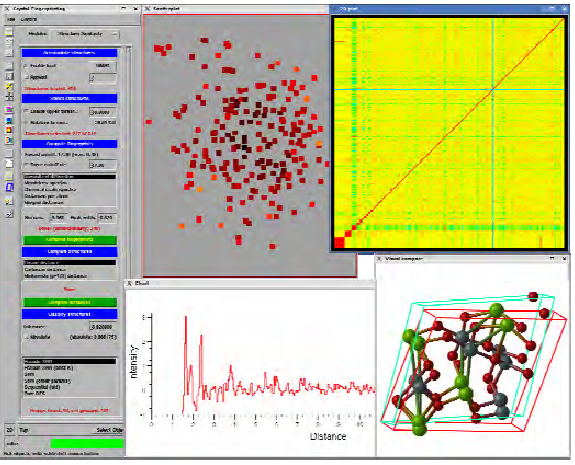
\includegraphics[scale=0.3]{pic/STM_screenshot.png} 
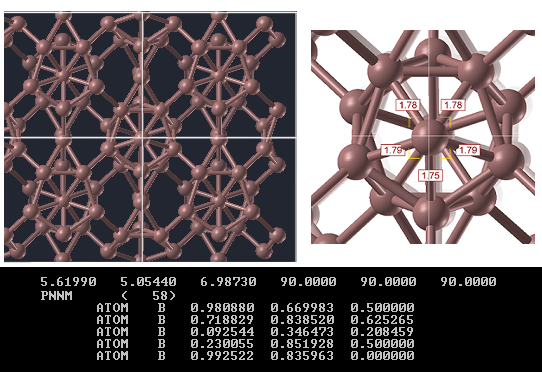
\includegraphics[scale=0.4]{pic/B_structure}
\caption{\footnotesize \textbf{STM4 interface for USPEX.}}
\label{fig:STM4}
\end{figure}

Alternatively, you can visualize USPEX results with other software, \emph{e.g.},
OpenDX, VESTA, \emph{etc.} VESTA already includes a feature for reading USPEX
structure files directly.

\subsection{How can I avoid trapping?} \label{faq_trapping}
First, use a sufficiently large population size. Second, USPEX by default uses a
powerful fingerprint niching method. Anything that increases the diversity of
the population will reduce the chances of trapping in a local minimum. To make
sure that your simulation is not trapped, it is useful to run a second
simulation with different parameters. A powerful trick to avoid trapping is the
antiseed technique.

\subsection{What is a single block calculation?} \label{faq_single_block}
The single block feature was introduced in USPEX~9.3.9, and enables USPEX users
to run structure predictions with a variable number of formula units 
of the same composition. For example:

{\footnotesize
\begin{verbatim}
% atomType
Si O
% EndAtomType

% numSpecies
1 2
% EndNumSpecies

12 : minAt
24 : maxAt
\end{verbatim}
}

This means we sample structures of compound SiO$_2$ (with the ratio of 1:2)
with a variable number of formula units with 12--24 atoms.

Starting from USPEX~9.4.1, the single block feature has been moved from
\keyword{calculationType} = 301/311 to 300/310. The settings are still the same,
users just need to set up the \keyword{minAt}, \keyword{maxAt} and
\keyword{numSpecies} keywords.


\subsection{How do I use the seed technique?} \label{faq_seeds}
This technique is useful, if instead of starting with random structures, you
would like to input some structures that you already know for the compound or
related materials. Just create a file \file{Seeds/POSCARS} for the next
generation, or \file{Seeds/POSCARS\_gen} (\texttt{gen} is the generation number)
for the specific generation of an USPEX calculation, in the format of
concatenated \file{POSCAR} files in VASP5 format. Don't miss letter
``\texttt{S}'' in the file name.

Example:

{\footnotesize
\begin{verbatim}
    EA33 2.69006 5.50602 4.82874 55.2408 73.8275 60.7535 no SG
    1.0
    2.690100  0.000000  0.000000
    2.690100  4.804100  0.000000
    1.344900  2.402100  3.967100
    Mg Al O
    1  2  4
    Direct
    0.799190  0.567840  0.859590
    0.793520  0.230950  0.544750
    0.793540  0.916090  0.174450
    0.050972  0.816060  0.859610
    0.172230  0.194810  0.859600
    0.438250  0.655170  0.406880
    0.438230  0.202440  0.312330
    EA34 7.61073 2.85726 2.85725 60.0001 79.1809 79.1805 no SG
    1.0
    7.610700  0.000000  0.000000
    0.536350  2.806500  0.000000
    0.536330  1.352000  2.459300
    Mg Al O
    1  2  4
    Direct
    0.708910  0.507440  0.068339
    0.374050  0.285730  0.846630
    0.023663  0.069185  0.630090
    0.889560  0.780560  0.341460
    0.350470  0.626920  0.187820
    0.597290  0.211310  0.772210
    0.116440  0.371590  0.932500
\end{verbatim}
}

One can add  seeds at any time during the calculation. USPEX will look for new
seeds at the beginning of each generation. The corresponding information will be
recorded to \file{results1/Seeds\_history} and the seeds files (\file{POSCARS}
or \file{POSCARS\_gen}) will be kept as \file{POSCARS\_gen} in \file{Seeds/}
folder.

Whenever seeds are added, we suggest users to check the
\file{results1/Seeds\_history} and \file{Warnings} files. There will be a
warning message ``\texttt{Meet a problem when reading Seeds - ...}'' if your
seeds are problematic. When an error appears in the seeds file, such as missing
lines, the structures after the error point will not be added.

\textbf{Note:} Make sure you specified all atomic symbols at the 6$^{th}$ line
of each structure. For example, to add the $P6_{3}/mc$ H$_2$ structure to a H-O
variable-composition calculation, you should edit the file as:

{\footnotesize
\begin{verbatim}
    H_I-P63/mc
    1
    4.754726  -2.74514  0.000000
    -0.00000  5.490285  0.000000
    0.000000  0.000000  4.508715
    H
    16
    Direct
    ...
    (the atomic positions information is omitted here)
\end{verbatim}
}

% We should teach USPEX to deal with this:
%It is very \textbf{IMPORTANT} that you write the oxygen name tag even if there
%are no oxygen atoms in the $P6_{3}/mc$ H$_2$ structure, otherwise USPEX will
%complain and skip the structure.


\subsection{How do I play with the compositions?}\label{faq_compositions}

For variable-composition and single block calculations, as soon as the
calculation starts, it produces a file \file{Seeds/compositions} with all
possible compositions, from which the code randomly takes compositions for the
random structure generator. You can edit this file, leaving the compositions you
are most interested in --- only these compositions will be used for random
structure production in the second and subsequent generations.
\file{Seeds/compositions} file lists the numbers of atoms of each type in the
cell, \emph{e.g.}, for the C-O system:

\begin{verbatim}
    8 0
    0 8
    2 4
\end{verbatim}

means that you are interested in randomly producing C$_8$, O$_8$, and C$_2$O$_4$
structures. Other compositions will be sampled too, thanks to the heredity and
transmutation operators.

When you want to generate structures with specific compositions, you can use the
anti-compositions feature --- write the list of all unwanted compositions to the
file named \file{Seeds/Anti-compositions}. There are three ways to do so:

\begin{enumerate}

\item For all unwanted compositions with the same ratios, you can write
stoichiometric ratio to ban these compositions. For example, you can use
``\texttt{1 2 1}'' to ban all the composition with the same ratio, such as
``\texttt{1 2 1}'', ``\texttt{2 4 2}'', ``\texttt{3 6 3}'' and so on.

\item Only for the specific composition, but not for other compositions with the
same ratio. You can write the compositions with a minus sign. For example, you
can use ``\texttt{-3 2 0}'' or ``\texttt{3 -2 0}'' to ban the ``\texttt{3 2 0}''
composition, but not to ban ``\texttt{6 4 0}'' or ``\texttt{9 6 0}''
composition. (Notice: ``\texttt{3 2 -0}'' does not work for this case).

\item For all single/binary/ternary compounds. If you don't want to sample all
single/binary/ternary compounds, just write the keyword
\keyword{single/binary/ternary} in \file{Anti-compositions} file.

\end{enumerate}

Example:

\begin{verbatim}
    single
    binary
    1 1 2
   -2 2 1
\end{verbatim}

If you don't clearly know what you are doing, please leave
\file{Anti-compositions} file empty. For more information about the compositions
you don't want, you can have a look at \file{results1/compositionStatistic}
file.

\textbf{Note:} 
\begin{itemize}

\item Even if \file{compositions} or \file{Anti-compositions} files exist before
the calculation starts, they will be ignored. \file{Anti-compositions} file will
be renamed to a backup file \file{Anti-compositions-back}. Therefore, please
edit \file{compositions} or \file{Anti-compositions} files after the calculation
starts.

\item Please also be aware, that in USPEX calculations with compositional
blocks, the compositions usually mean the numbers of these blocks. Therefore, to
have the correct format of \file{Anti-compositions} file, please check
\file{compositions} file first.

\end{itemize}

\subsection{How do I set up a passwordless connection from a local machine to a
remote cluster?} \label{faq_passwordless}

You will need to copy the public key from your local machine (directory
\file{./ssh} or \file{./ssh2}) to the remote cluster.
Here is the list of commands you need to execute:

{\footnotesize
\begin{verbatim}
local # ssh-keygen -t dsa
local # scp ~/.ssh2/id_dsa.pub oganov@palu.cscs.ch:~/.ssh/tmp.pub
remote # cd ~/.ssh/
remote # ssh-keygen -f tmp.pub -i >> authorized_keys
remote # rm tmp.pub
\end{verbatim}
}

\subsection{How do I restart a calculation with a corrupt \file{*.mat} file?}
\label{faq_mat_files}

When there is a problem in file system, e.g. the disk is full, the file system
is overloaded, USPEX could have a problem in writing these \file{*.mat} files
correctly, and meet a message during the calculation like:

\begin{verbatim}
 ???Error using ==> load
 Unable to read MAT file /home/USPEX/Current_POP.mat
 
 File may be corrupt.
\end{verbatim}

When you meet an error with a corrupt \file{*.mat} file, please recover the
broken \file{*.mat} file with the backup one, delete the \file{matfilelocker}
file, then restart the calculation. Unfortunately, when the backup \file{*.mat}
file is empty or also corrupt, you have to restart the calculation with a
generation pickup.

\subsection{What should I do when USPEX is not running for a while?}
\label{faq_uspex_hang}

When you found USPEX is not running for a while, with file \file{still\_running}
existing for a long time (usually longer than 30 minutes; use ``\texttt{ls -l}''
command to check the timestamp of the \file{still\_running} file), you should
consider that there is something wrong with the calculation. In this situation,
what you need to do is to follow a checking procedure below:

\begin{itemize}

\item Make sure your MATLAB calculation is not running, use ``\texttt{top}''
command to check it. Sometimes USPEX can take long time in structure generation
and softmutation. Once you are sure that MATLAB stopped, you can continue with
the next step.

\item Stop your crontab or job running script to avoid USPEX running during the
checking procedure. This is very important, otherwise you will mess up your
USPEX calculations.

\item Delete the \file{still\_running} file.

\item Run USPEX with command ``\texttt{USPEX -r}'' or ``\texttt{matlab <
USPEX.m}'' to check what will happen. If you meet errors or bugs, you can try to
fix them, or report a bug to our USPEX Google forum.

\item If everything is fine, just restart your crontab or job running script to
continue the calculation.

\end{itemize}

\subsection{How do I set up a calculation using a job submission script?}
\label{faq_job_submit}

To set up a job submission script, we expect users to know some basic knowledge
of MATLAB programing and your job submission systems, at least the basic idea of
how to work with strings in MATLAB and how to get the job information.

There are two modes for job submission: \textbf{local} submission or
\textbf{remote} submission, depending on whether you submit \emph{ab initio}
calculations to the local machine where you run USPEX and MATLAB, or to a remote
supercomputer.

\subsubsection{Step 1: Configuring files in \file{Submission/} folder}

\textbf{Case I: Local submission. }

Please edit in \file{INPUT.txt} file the following tag:

{\footnotesize
\begin{verbatim}
1   : whichCluster (0: no-job-script, 1: local submission, 2: remote submission)
\end{verbatim}}

Then, go to the directory \file{Submission/}, where you need to edit two files:
\file{submitJob\_local.m} and \file{checkStatus\_local.m}.

One can find the detailed instructions in these files. In general, one just
needs to tell USPEX how to submit the job and check if the job has completed or
not.

\vspace{0.5cm}
In \file{submitJob\_local.m}:
%{\footnotesize
%\begin{verbatim}

\begin{lstlisting}
function jobNumber = submitJob_local()
%-------------------------------------------------------------
%This routine is to check if the submitted job is complete or not
%One needs to do a little edit based on your own situation.
%1   : whichCluster (default 0, 1: local submission, 2: remote submission)
%-------------------------------------------------------------

%Step 1: to prepare the job script that is required by your supercomputer
fp = fopen('myrun', 'w');    
fprintf(fp, '#!/bin/sh\n');
fprintf(fp, '#PBS -l nodes=1:ppn=8,walltime=1:30:00 -q cfn_short\n');
fprintf(fp, '#PBS -N USPEX\n');
fprintf(fp, '#PBS -j oe\n');
fprintf(fp, '#PBS -V \n');
fprintf(fp, 'cd ${PBS_O_WORKDIR}\n');
fprintf(fp, 'mpirun -np 4 vasp1 > vasp.out\n');
fclose(fp);

%Step 2: to submit the job with a command like qsub, bsub, llsubmit, etc.

[a,b]=unix(['qsub myrun'])

%Step 3: to get the jobID from the screen message
%It will output some message on the screen like '2350873.nano.cfn.bnl.local'

end_marker = findstr(b,'.');
jobNumber = b(1:end_marker(1)-1); 
\end{lstlisting}
%\end{verbatim}
%}

In \file{checkStatus\_local.m}:
%{\footnotesize
%\begin{verbatim}
\begin{lstlisting}
function doneOr = checkStatus_local(jobID)
%--------------------------------------------------------------------
%This routine is to check if the submitted job is complete or not
%One needs to do a little edit based on your own case.
1   : whichCluster (0: no-job-script, 1: local submission, 2: remote submission)
%--------------------------------------------------------------------

%Step1: the command to check job by ID. 
    [a,b] = unix(['qstat ' jobID ''])

%Step2: to find the keywords from the screen message to determine if the job is complete
%Below is just a sample:
%-------------------------------------------------------------------------------
%Job id                    Name             User            Time Use S Queue
%------------------------- ---------------- --------------- -------- - ---------
%2455453.nano              USPEX            qzhu            02:28:42 R cfn_gen04
%-------------------------------------------------------------------------------
%If the job is still running, it will show as above.
%If there are no key words like 'Q/R Cfn_gen04', it indicates the job is complete.
%Therefore, we can use a small MATLAB function findstr to apply this argument.
    if isempty(findstr(b,'R cfn_')) & isempty(findstr(b,'Q cfn_'))   
       doneOr = 1
       unix('rm USPEX*');    % to remove the log file
	end
\end{lstlisting}
%\end{verbatim}
%}

\textbf{Case II: Remote submission.}

Please edit in \file{INPUT.txt} file the following tag:

{\footnotesize
\begin{verbatim}
2       : whichCluster (default 0, 1: local submission; 2: remote submission)
C-20GPa : remoteFolder
\end{verbatim}
}

Finally, go to the directory \file{Submission/}, where you need to edit two
files: \\
\file{submitJob\_remote.m} and \file{checkStatus\_remote.m}

\newpage
In \file{submitJob\_remote.m}:
%{\footnotesize
%\begin{verbatim}
\begin{lstlisting}
function jobNumber = submitJob_remote(USPEX, Index)
%-------------------------------------------------------------
%This routine is to check if the submitted job is complete or not
%2   : whichCluster (default 0, 1: local submission; 2: remote submission)
%C-20GPa : remoteFolder
%-------------------------------------------------------------

%-------------------------------------------------------------
%Step1: To prepare the job script, runvasp.sh
  fp = fopen('runvasp.sh', 'w');
  fprintf(fp, '#!/bin/sh\n');
  fprintf(fp, '#PBS -l nodes=2:ppn=2,walltime=1:30:00\n');
  fprintf(fp, '#PBS -N USPEX\n');
  fprintf(fp, '#PBS -j oe\n');
  fprintf(fp, '#PBS -V \n');
  fprintf(fp, 'cd ${PBS_O_WORKDIR}\n');
  fprintf(fp, '/usr/local/pkg/openmpi-1.4.5/bin/mpirun -np 4 vasp1 > vasp.out\n');
  fclose(fp);
%-------------------------------------------------------------------------------
%Step 2: Copy the files to the remote machine

%Step2-1: Specify the PATH to put your calculation folder
Home = ['/nfs/user08/qiazhu']; %'pwd' of your home directory on remote machine
Address = 'qiazhu@seawulf.stonybrook.edu'; %your target server: username@address
Path = [Home '/' USPEX '/CalcFold' num2str(Index)];  %Just keep it

%Step2-2: Create the remote directory 
% Please change the ssh/scp command if necessary! 
% Sometimes you don't need the -i option
try
[a,b]=unix(['ssh -i ~/.ssh/seawulf ' Address ' mkdir ' USPEX ]);  
catch
end

try
[a,b]=unix(['ssh -i ~/.ssh/seawulf ' Address ' mkdir ' Path ]);
catch
end

%Step2-3: Copy the necessary files (for VASP calculations, we need POSCAR, INCAR, POTCAR,
% KPOINTS and job script)
unix(['scp -i ~/.ssh/seawulf POSCAR   ' Address ':' Path]);
unix(['scp -i ~/.ssh/seawulf INCAR    ' Address ':' Path]);
unix(['scp -i ~/.ssh/seawulf POTCAR   ' Address ':' Path]);
unix(['scp -i ~/.ssh/seawulf KPOINTS  ' Address ':' Path]);
unix(['scp -i ~/.ssh/seawulf runvasp.sh ' Address ':' Path]);

%------------------------------------------------------------------------------
%Step 3: to submit the job and get JobID, i.e., the exact command to submit the job.
[a,v]=unix(['ssh -i ~/.ssh/seawulf ' Address ' /usr/local/pkg/torque/bin/qsub ' 
           Path '/runvasp.sh'])

% format: Job 1587349.nagling is submitted to default queue <mono>
end_marker = findstr(v,'.');
if strfind(v,'error')
   jobNumber=0;
else
   jobNumber = v(1:end_marker(1)-1);
end
\end{lstlisting}
%\end{verbatim}
%}

\newpage
In \file{CheckStatus\_remote.m}:
%{\footnotesize
%\begin{verbatim}

\begin{lstlisting}
function doneOr = checkStatus_remote(jobID, USPEX, Folder)
%--------------------------------------------------------------------
%This routine is to check if the submitted job is complete or not
%One needs to do a little edit based on your own situation.
%--------------------------------------------------------------------

%Step1: Specify the PATH to put your calculation folder
Home = ['/nfs/user08/qiazhu']; %'pwd' of your home directory of your remote machine
Address = 'qiazhu@seawulf.stonybrook.edu';  %Your target: username@address.
Path = [Home '/' USPEX '/CalcFold' num2str(Folder)]; %just keep it
%Step2: Check JobID, the exact command to check job by jobID
[a,b]=unix(['ssh -i ~/.ssh/seawulf ' Address ' /path/to/qstat ' num2str(jobID)])
    tempOr1 = strfind(b, 'R batch');
    tempOr2 = strfind(b, 'Q batch');
    if isempty(tempOr1) & isempty(tempOr2)
      doneOr = 1;
% for vasp, we usually need OSZICAR for reading energy and CONTCAR for reading 
%structure OUTCAR, EIGENVAL, DOSCAR might be needed for reading other properties.
%   unix(['scp -i ~/.ssh/seawulf ' Address ':' Path '/OUTCAR ./']) 
%OUTCAR is not necessary by default
      unix(['scp -i ~/.ssh/seawulf ' Address ':' Path '/OSZICAR ./']) 
%For reading enthalpy/energy
      unix(['scp -i ~/.ssh/seawulf ' Address ':' Path '/CONTCAR ./']) 
%For reading structural info
end
\end{lstlisting}
%\end{verbatim}
%}

It might take some time to correctly configure these files. To test if it works
or not, you can type ``\texttt{USPEX -r}'' twice and then track the
screen information. The first attempt is to check if the jobs are submitted,
while the second attempt is to check if USPEX can correctly check the status of
the submitted jobs. All of the related information can be found in the screen
output message. If MATLAB exits without any errors, you are almost ready to go.

\subsubsection{Step 2: Running USPEX periodically}

The real calculation starts with the command ``\texttt{USPEX -r > log}''. Each
time the MATLAB process will check the status of the running \emph{ab initio}
calculations. If the job is complete, MATLAB will go the the calculation folder
to read the results, and then submit new calculations. After that, MATLAB will
exit. Therefore, one needs to periodically call the command (for example, every
5 minutes). The periodic script can be executed by using either \texttt{crontab}
or a shell script.

\subsubsection{Crontab}
This can be performed using a \texttt{crontab} daemon on your Linux machine. In
your user home directory, there should now be the files:

\lstset{language=csh, frame=None, basicstyle=\footnotesize}
\begin{verbatim}
~/call_job
~/CronTab
\end{verbatim}

Here is an example of a 1-line \file{CronTab} file from one of our clusters:

%\begin{verbatim}
\begin{lstlisting}
*/5 * * * * sh call_job
\end{lstlisting}
%\end{verbatim}

It states that the interval between job submissions is 5 minutes and points to
the file \file{call\_job}, which should contain the address of the directory
where USPEX will be executed, and the file \file{call\_job} looks like this:

%\begin{verbatim}
\begin{lstlisting}
#!/bin/sh
source $HOME/.bashrc
cd /ExecutionDirectory
date >> log
USPEX -r >> log
\end{lstlisting}
%\end{verbatim}

To activate \keyword{crontab}, type

%\begin{verbatim}
\begin{lstlisting}
crontab ~/CronTab
\end{lstlisting}
%\end{verbatim}

If you want to terminate this run, either edit \file{call\_job} or remove this
\keyword{crontab} by typing

%\begin{verbatim}
\begin{lstlisting}
crontab -r
\end{lstlisting}
%\end{verbatim}

To check if crontab works well, one should also keep tracking the updates of the
log file at the beginning of the calculation.

\subsubsection{Shell script}
You can also prepare the script by using the \keyword{sleep} command in Linux
shell. Below is a rather simple script \file{run-uspex.sh}:

%\begin{verbatim}
\begin{lstlisting}
#!/bin/sh
while [ ! -f ./USPEX_IS_DONE ]; do
   date >> log 
   USPEX -r >> log
   sleep 300
done
\end{lstlisting}
%\end{verbatim}

\textbf{Note:} keep in mind that this calculation can only be terminated by
killing the process ID of this script.


\subsection{How do I work with symmetry codes on 32-bit machines?}
\label{faq_32bit}
Execute ``\file{./install-32bit.sh}'' shell script under
\file{FunctionFolder/Tool/32bit/} folder to replace the default 64-bit binary
codes by the 32-bit executables.


%%%%%%%%%%%%%%%%%%%%%%%%%%%%%%%%%%%%%%%%%%%%%%%%%%%%%%%%%%%%%%%%%%%%%%%%%%%%%%%%
\newpage
\section{Appendices}

\subsection{List of Examples} \label{appendix_examples}

\begin{itemize}
\item  \texttt{EX01-3D\_Si\_vasp}: Silicon (8 atoms/cell) at zero pressure.
Variable-cell DFT calculation using VASP, PBE96 functional. Many thanks to
G.~Kresse for permission to include his PAW files (\file{POTCAR}) in our
distribution.

\item \texttt{EX02-3D\_MgAl2O4\_gulp}: MgAl$_2$O$_4$ (28 atoms/cell) at
100~GPa pressure. Variable-cell calculation using Buckingham potentials, GULP
code. Beware that for reliable, you should better do \emph{ab initio}
calculations.

\item \texttt{EX03-3D-const\_cell\_MgSiO3\_gulp}: this example shows how to do
structure prediction when you know cell parameters. MgSiO$_3$ (20 atoms/cell)
with Buckingham potentials, GULP code. Cell parameters correspond to
post-perovskite. The discovery of post-perovskite (\textit{Oganov \& Ono, Nature
2004; Murakami et al., Science 2004}) was a major breakthrough in Earth
sciences.

\item \texttt{EX04-3D\_C\_lammps}: this example shows how to do crystal
structure prediction using USPEX together with the LAMMPS code. In this a simple
example: 8 carbon atoms, and Tersoff potential.

\item \texttt{EX05-3D\_Si\_atk}: Example of crystal structure prediction of Si
with 8 atoms/cell using the density-functional tight binding approximation and
ATK code.

\item \texttt{EX06-3D\_C\_castep}: DFT-based prediction of the crystal structure
of carbon with 8 atoms/cell at 10~GPa, using the CASTEP code.

\item \texttt{EX07-2D\_Si\_vasp}: prediction of the 2D-crystal of silicon using
DFT and VASP. Simple and powerful.

\item \texttt{EX08-0D\_LJ\_gulp}: Nanoparticle structure prediction.
Lennard-Jones nanoparticle with 30 atoms, using the GULP code.

\item \texttt{EX09-3D-molecules\_CH4\_vasp}: methane with 4 molecules/cell,
at the pressure of 20~GPa. DFT, VASP. Molecule is described in the file
\file{MOL\_1}.

\item \texttt{EX10-3D-molecules\_CH4\_dmacrys}: methane with 8
molecules/cell, with forcefield and DMACRYS code, at normal pressure. Molecule
is described in the file \file{MOL\_1}, but note its slightly unusual format for
DMACRYS calculations. Please put executables \file{dmacrys},
\file{neighcrys-pp}, \file{neighcrys-vv} in the \file{Specific/} folder.

\item \texttt{EX11-3D-molecules\_urea\_tinker}: urea with 2 molecules/cell, with
forcefield and TINKER code, at normal pressure. Molecule is described in the
file \file{MOL\_1}.

\item \texttt{EX12-3D\_varcomp\_LJ\_gulp}: Lennard-Jones binary system with fake
``Mo'' and ``B'' atoms, GULP, and variable-composition USPEX (\textit{Lyakhov
and Oganov, 2010}).

\item \texttt{EX13-3D\_special\_quasirandom\_structure\_TiCoO}: USPEX can easily
find the most disordered (or the most ordered) alloy structure. Here, this is
shown for Ti$_x$Co$_{(1-x)}$O. You need to specify the initial structure in
\file{Seeds/POSCARS} and use only the permutation operator. In this case, you
don't need to use any external codes. In this example, we optimize (minimize)
the structural order (\textit{Oganov and Valle (2009); Lyakhov, Oganov, Valle
(2010)}) without relaxation (\keyword{abinitioCode} = 0). Seed structure
(supercell of Ti-Co-O-structure) is permutated to find the structure the
minimum/maximum order. Minimizing order in this situation, one gets a
generalized version of the ``special quasirandom structure''.

\item \texttt{EX14-GeneralizedMetadynamics\_Si\_vasp}: simple example of a
powerful capability to find complex low-energy structures starting with a simple
seed structure (\textit{Zhu et al, 2013}). Silicon, up to 16 atoms/cell, DFT,
VASP. Pay special attention to \file{INCAR} files. Best of all, just keep the
files that you see here, changing only \keyword{ENCUT}, perhaps \keyword{SIGMA}.
Evolutionary metadynamics not only predicts low-energy structures, but also
gives an idea of transition mechanisms between crystal structures.

\item \texttt{EX15-VCNEB\_Ar\_gulp}: example of a variable-cell nudged elastic
band (\textit{VCNEB: Qian et al., 2013}) calculation fcc-hcp transition in a
model system, argon, at 0~GPa pressure. Lennard-Jones potential, GULP code.

\item \texttt{EX16-USPEX-performance\_SrTiO3\_gulp}: SrTiO$_3$ (50 atoms/cell)
at zero pressure. Variable-cell calculation using Buckingham potentials, GULP
code. Running this example you can see that even for such a relatively large
system USPEX code scores a $>$90\% success rate and remarkable efficiency. This
contrasts with a 7-12\% success rate reported for the same system and using the
same potential by Zurek \& Lonie. Clearly, USPEX outperforms the poor
reimplementation of our method by Zurek and Lonie. We have witnessed excellent
performance of our code also for much larger systems.

\item \texttt{EX17-3D\_DebyeTemp\_C\_vasp}: example of optimization of the
elasticity-related properties (bulk or shear moduli, Poisson ratio, Chen-Niu
hardness, or Debye temperature). In this example, we maximize the Debye
temperature of carbon using the VASP code.

\item \texttt{EX18-3D\_varcomp\_ZnOH\_gulp}: as you know, USPEX has unique
capabilities for variable-composition searches. This example shows a pretty
challenging case --- variable-composition calculation for the ternary system
Zn-O-H. This calculation uses a ReaxFF forcefield in GULP code. USPEX can do
calculations for any number of components --- \emph{e.g.} quaternary,
quinternary, \emph{etc.} systems are within its reach. Of course, the more
components you have, the more expensive (and the more risky) your calculation
is. No reference results at the moment.

\item \texttt{EX19-Surface-boron111}: Prediction of (111) surface reconstruction
of alpha-boron, with variable number of atoms (Zhou \emph{et al.}, Phys. Rev.
Lett. 113, 176101 (2014)).

\item \texttt{EX20-0D\_Cluster\_C60\_MOPAC}: Cluster structure prediction (000)
for C$_{60}$ using MOPAC.

\item \texttt{EX21-META\_MgO\_gulp}: Evolutionary metadynamics, with GULP code
and Buckingham potentials, MgO with 8~atoms/cell. Starting structure is of
rocksalt type, and evolutionary metadynamics finds a number of low-energy
structures and structural relations.

\item \texttt{EX22-GEM\_MgO\_gulp}: Generalized evolutionary metadynamics, with
GULP code and Buckingham potentials. Starting structure is of rocksalt type,
with 8~atoms/cell, the calculation is allowed to increase system size up to
16~atoms/cell, and generalized evolutionary metadynamics (GEM) finds a number of
low-energy structures and structural relations.

\end{itemize}

\newpage
\subsection{Test runs}

\begin{figure}[htbp] \centering
	\begin{tabular}{c c}
		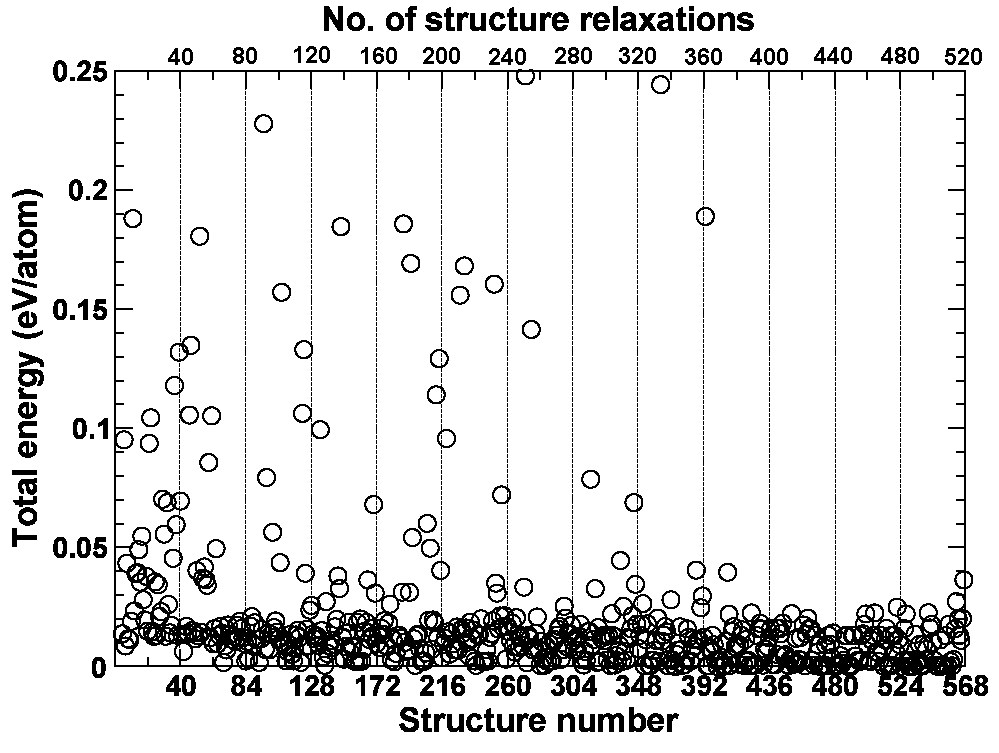
\includegraphics[scale=0.2]{pic/testrun_a} &
		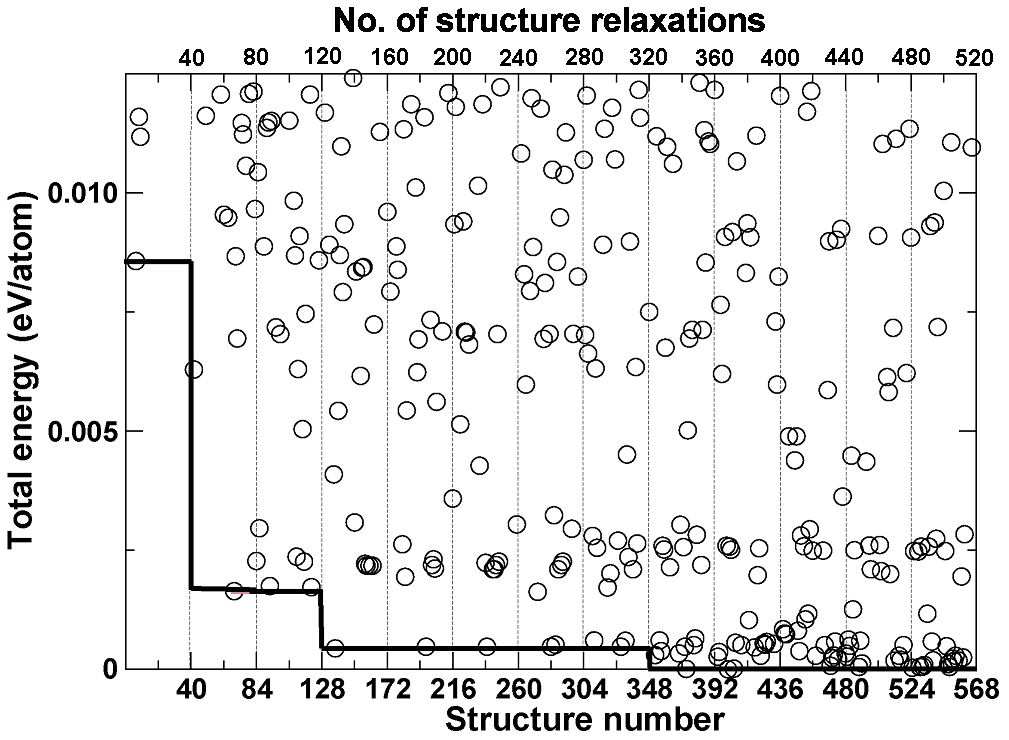
\includegraphics[scale=0.2]{pic/testrun_b} \\
		(a) & (b) \\
		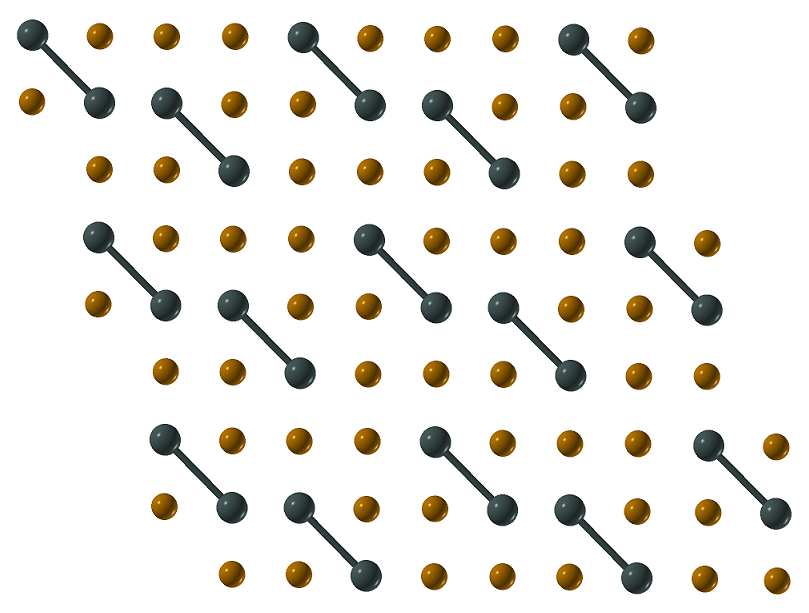
\includegraphics[scale=0.25]{pic/testrun_c} &
		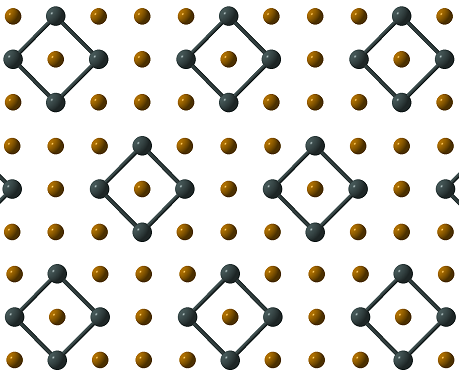
\includegraphics[scale=0.35]{pic/testrun_d} \\
		(c) & (d)
	\end{tabular}
\caption[]{\footnotesize
\textbf{Evolutionary structure search for Au$_8$Pd$_4$.} a, b --- evolution of
the total energy (for clarity, panel (b) zooms in on the lowest-energy region of
the same data set), c --- the lowest-energy structure found in our evolutionary
simulation, and d --- the lowest-energy structure found by cluster expansion
calculations of Zunger. Note that our structure (c) is the lowest-energy known
structure for this compound. This establishes the power of our method (even in
its ancient, 2007, version).}
\end{figure}

%%%%%%%%%%%%%%%%%%%%%%%%%%%%%%%%%%%%%%%%%%%%%%%%%%%%%%%%%%%%%%%%%%%%%%%%%%%%%%%%
\newpage
\subsection{Sample \file{INPUT.txt} files} \label{appendix_input_files}

\subsubsection{Fixed-composition USPEX calculation
(\keyword{calculationType}=300):}

\lstset{language=MATLAB, frame=single, basicstyle=\small}
\begin{lstlisting}
PARAMETERS EVOLUTIONARY ALGORITHM
% Example of the short input, using most options as defaults

% atomType
Mg Al O
% EndAtomType

% numSpecies
2 4 8
% EndNumSpecies

50   : numGenerations 
50.0 : ExternalPressure

% abinitioCode 
3 3 3 3 3
% ENDabinit

% commandExecutable
gulp < input > output
% EndExecutable
\end{lstlisting}

\newpage
\subsubsection{Variable-composition USPEX calculation
(\keyword{calculationType}=301):}

\lstset{language=MATLAB, frame=single, basicstyle=\small}
\begin{lstlisting}
USPEX : calculationMethod (USPEX, VCNEB, META)
301   : calculationType (dimension: 0-3; molecule: 0/1; varcomp: 0/1)
1     : AutoFrac

% atomType
Mo B
% EndAtomType

% numSpecies
1 0
0 1
% EndNumSpecies

80    : populationSize
200   : initialPopSize
60    : numGenerations 
20    : stopCrit

11    : firstGeneMax 
8     : minAt
18    : maxAt

% abinitioCode 
3 3 3
% ENDabinit

% commandExecutable
gulp < input > output
% EndExecutable
\end{lstlisting}


\newpage
\subsubsection{Evolutionary metadynamics (\keyword{calculationMethod}=META):}

\lstset{language=MATLAB, frame=single, basicstyle=\small}
\begin{lstlisting}
META  : calculationMethod (USPEX, VCNEB, META)
301   : calculationType (dimension: 0-3; molecule: 0/1; varcomp: 0/1)

% valences
4
% endValences

% IonDistances
1.2
% EndDistances

0.0001 : ExternalPressure

16    : maxAt
2.0   : minVectorLength 
8.0   : maxVectorLength

15    : populationSize
40    : numGenerations
3.0   : mutationDegree
250.0 : GaussianHeight
0.3   : GaussianWidth
2     : FullRelax

abinitioCode 
1 1 1 (1 1)
ENDabinit

% KresolStart
0.12 0.10 0.09 0.10 0.08
% Kresolend

% commandExecutable
mpirun -np 4 vasp > log
% EndExecutable
\end{lstlisting}

\newpage
\subsubsection{vcNEB calculation
(\keyword{calculationMethod}=VCNEB):}

\lstset{language=MATLAB, frame=single, basicstyle=\small}
\begin{lstlisting}
VCNEB : calculationMethod

% numSpecies
4
% EndNumSpecies

% atomType
Ar
% EndAtomType

0.0   : ExternalPressure

111   : vcnebType   
15    : numImages
500   : numSteps
1     : optimizerType
2     : optReadImages
3     : optRelaxType
0.25  : dt
0.003 : ConvThreshold

0.3   : VarPathLength
3     : K_min
6     : K_max
0     : optFreezing
0     : optMethodCIDI

2     : FormatType 
10    : PrintStep

abinitioCode
3
ENDabinit

% commandExecutable
gulp < input > output
% EndExecutable
\end{lstlisting}

%%%%%%%%%%%%%%%%%%%%%%%%%%%%%%%%%%%%%%%%%%%%%%%%%%%%%%%%%%%%%%%%%%%%%%%%%%%%%%%%
\newpage
\subsection{List of space groups} \label{appendix_space_groups}

\begin{center}
{\scriptsize
\begin{tabular}{|r|l||r|l||r|l||r|l|}
\hline
   1 & $P1$                                   &   2 & $P\mbox{-}1$                           &   3 & $P2$                                   &   4 & $P2_{1}$                               \\
   5 & $C2\ (A2)$\footnotemark[1]             &   6 & $Pm$                                   &   7 & $Pc\ (Pa)$\footnotemark[1]             &   8 & $Cm\ (Am)$\footnotemark[1]             \\
   9 & $Cc\ (Aa)$\footnotemark[1]             &  10 & $P2/m$                                 &  11 & $P2_{1}/m$                             &  12 & $C2/m\ (A2/m)$\footnotemark[1]         \\
  13 & $P2/c\ (P2/a)$\footnotemark[1]         &  14 & $P2_{1}/c\ (P2_{1}/a)$\footnotemark[1] &  15 & $C2/c\ (A2/a)$\footnotemark[1]         &  16 & $P222$                                 \\
  17 & $P222_{1}$                             &  18 & $P2_{1}2_{1}2$                         &  19 & $P2_{1}2_{1}2_{1}$                     &  20 & $C222_{1}$                             \\
  21 & $C222$                                 &  22 & $F222$                                 &  23 & $I222$                                 &  24 & $I2_{1}2_{1}2_{1}$                     \\
  25 & $Pmm2$                                 &  26 & $Pmc2_{1}$                             &  27 & $Pcc2$                                 &  28 & $Pma2$                                 \\
  29 & $Pca2_{1}$                             &  30 & $Pnc2$                                 &  31 & $Pmn2_{1}$                             &  32 & $Pba2$                                 \\
  33 & $Pna2_{1}$                             &  34 & $Pnn2$                                 &  35 & $Cmm2$                                 &  36 & $Cmc2_{1}$                             \\
  37 & $Ccc2$                                 &  38 & $Amm2\ (C2mm)$\footnotemark[1]         &  39 & $Aem2\ (C2mb)$\footnotemark[1]         &  40 & $Ama2\ (C2cm)$\footnotemark[1]         \\
  41 & $Aea2\ (C2cb)$\footnotemark[1]         &  42 & $Fmm2$                                 &  43 & $Fdd2$                                 &  44 & $Imm2$                                 \\
  45 & $Iba2$                                 &  46 & $Ima2$                                 &  47 & $Pmmm$                                 &  48 & $Pnnn$                                 \\
  49 & $Pccm$                                 &  50 & $Pban$                                 &  51 & $Pmma$                                 &  52 & $Pnna$                                 \\
  53 & $Pmna$                                 &  54 & $Pcca$                                 &  55 & $Pbam$                                 &  56 & $Pccn$                                 \\
  57 & $Pbcm$                                 &  58 & $Pnnm$                                 &  59 & $Pmmn$                                 &  60 & $Pbcn$                                 \\
  61 & $Pbca$                                 &  62 & $Pnma$                                 &  63 & $Cmcm$                                 &  64 & $Cmce\ (Cmca)$\footnotemark[1]         \\
  65 & $Cmmm$                                 &  66 & $Cccm$                                 &  67 & $Cmme\ (Cmma)$\footnotemark[1]         &  68 & $Ccce\ (Ccca)$\footnotemark[1]         \\
  69 & $Fmmm$                                 &  70 & $Fddd$                                 &  71 & $Immm$                                 &  72 & $Ibam$                                 \\
  73 & $Ibca$                                 &  74 & $Imma$                                 &  75 & $P4$                                   &  76 & $P4_{1}$                               \\
  77 & $P4_{2}$                               &  78 & $P4_{3}$                               &  79 & $I4$                                   &  80 & $I4_{1}$                               \\
  81 & $P\mbox{-}4$                           &  82 & $I\mbox{-}4$                           &  83 & $P4/m$                                 &  84 & $P4_{2}/m$                             \\
  85 & $P4/n$                                 &  86 & $P4_{2}/n$                             &  87 & $I4/m$                                 &  88 & $I4_{1}/a$                             \\
  89 & $P422$                                 &  90 & $P42_{1}2$                             &  91 & $P4_{1}22$                             &  92 & $P4_{1}2_{1}2$                         \\
  93 & $P4_{2}22$                             &  94 & $P4_{2}2_{1}2$                         &  95 & $P4_{3}22$                             &  96 & $P4_{3}2_{1}2$                         \\
  97 & $I422$                                 &  98 & $I4_{1}22$                             &  99 & $P4mm$                                 & 100 & $P4bm$                                 \\
 101 & $P4_{2}cm$                             & 102 & $P4_{2}nm$                             & 103 & $P4cc$                                 & 104 & $P4nc$                                 \\
 105 & $P4_{2}mc$                             & 106 & $P4_{2}bc$                             & 107 & $I4mm$                                 & 108 & $I4cm$                                 \\
 109 & $I4_{1}md$                             & 110 & $I4_{1}cd$                             & 111 & $P\mbox{-}42m$                         & 112 & $P\mbox{-}42c$                         \\
 113 & $P\mbox{-}42_{1}m$                     & 114 & $P\mbox{-}42_{1}c$                     & 115 & $P\mbox{-}4m2$                         & 116 & $P\mbox{-}4c2$                         \\
 117 & $P\mbox{-}4b2$                         & 118 & $P\mbox{-}4n2$                         & 119 & $I\mbox{-}4m2$                         & 120 & $I\mbox{-}4c2$                         \\
 121 & $I\mbox{-}42m$                         & 122 & $I\mbox{-}42d$                         & 123 & $P4/mmm$                               & 124 & $P4/mcc$                               \\
 125 & $P4/nbm$                               & 126 & $P4/nnc$                               & 127 & $P4/mbm$                               & 128 & $P4/mnc$                               \\
 129 & $P4/nmm$                               & 130 & $P4/ncc$                               & 131 & $P4_{2}/mmc$                           & 132 & $P4_{2}/mcm$                           \\
 133 & $P4_{2}/nbc$                           & 134 & $P4_{2}/nnm$                           & 135 & $P4_{2}/mbc$                           & 136 & $P4_{2}/mnm$                           \\
 137 & $P4_{2}/nmc$                           & 138 & $P4_{2}/ncm$                           & 139 & $I4/mmm$                               & 140 & $I4/mcm$                               \\
 141 & $I4_{1}/amd$                           & 142 & $I4_{1}/acd$                           & 143 & $P3$                                   & 144 & $P3_{1}$                               \\
 145 & $P3_{2}$                               & 146 & $R3$                                   & 147 & $P\mbox{-}3$                           & 148 & $R\mbox{-}3$                           \\
 149 & $P312$                                 & 150 & $P321$                                 & 151 & $P3_{1}12$                             & 152 & $P3_{1}21$                             \\
 153 & $P3_{2}12$                             & 154 & $P3_{2}21$                             & 155 & $R32$                                  & 156 & $P3m1$                                 \\
 157 & $P31m$                                 & 158 & $P3c1$                                 & 159 & $P31c$                                 & 160 & $R3m$                                  \\
 161 & $R3c$                                  & 162 & $P\mbox{-}31m$                         & 163 & $P\mbox{-}31c$                         & 164 & $P\mbox{-}3m1$                         \\
 165 & $P\mbox{-}3c1$                         & 166 & $R\mbox{-}3m$                          & 167 & $R\mbox{-}3c$                          & 168 & $P6$                                   \\
 169 & $P6_{1}$                               & 170 & $P6_{5}$                               & 171 & $P6_{2}$                               & 172 & $P6_{4}$                               \\
 173 & $P6_{3}$                               & 174 & $P\mbox{-}6$                           & 175 & $P6/m$                                 & 176 & $P6_{3}/m$                             \\
 177 & $P622$                                 & 178 & $P6_{1}22$                             & 179 & $P6_{5}22$                             & 180 & $P6_{2}22$                             \\
 181 & $P6_{4}22$                             & 182 & $P6_{3}22$                             & 183 & $P6mm$                                 & 184 & $P6cc$                                 \\
 185 & $P6_{3}cm$                             & 186 & $P6_{3}mc$                             & 187 & $P\mbox{-}6m2$                         & 188 & $P\mbox{-}6c2$                         \\
 189 & $P\mbox{-}62m$                         & 190 & $P\mbox{-}62c$                         & 191 & $P6/mmm$                               & 192 & $P6/mcc$                               \\
 193 & $P6_{3}/mcm$                           & 194 & $P6_{3}/mmc$                           & 195 & $P23$                                  & 196 & $F23$                                  \\
 197 & $I23$                                  & 198 & $P2_{1}3$                              & 199 & $I2_{1}3$                              & 200 & $Pm\mbox{-}3$                          \\
 201 & $Pn\mbox{-}3$                          & 202 & $Fm\mbox{-}3$                          & 203 & $Fd\mbox{-}3$                          & 204 & $Im\mbox{-}3$                          \\
 205 & $Pa\mbox{-}3$                          & 206 & $Ia\mbox{-}3$                          & 207 & $P432$                                 & 208 & $P4_{2}32$                             \\
 209 & $F432$                                 & 210 & $F4_{1}32$                             & 211 & $I432$                                 & 212 & $P4_{3}32$                             \\
 213 & $P4_{1}32$                             & 214 & $I4_{1}32$                             & 215 & $P\mbox{-}43m$                         & 216 & $F\mbox{-}43m$                         \\
 217 & $I\mbox{-}43m$                         & 218 & $P\mbox{-}43n$                         & 219 & $F\mbox{-}43c$                         & 220 & $I\mbox{-}43d$                         \\
 221 & $Pm\mbox{-}3m$                         & 222 & $Pn\mbox{-}3n$                         & 223 & $Pm\mbox{-}3n$                         & 224 & $Pn\mbox{-}3m$                         \\
 225 & $Fm\mbox{-}3m$                         & 226 & $Fm\mbox{-}3c$                         & 227 & $Fd\mbox{-}3m$                         & 228 & $Fd\mbox{-}3c$                         \\
 229 & $Im\mbox{-}3m$                         & 230 & $Ia\mbox{-}3d$                         &     &                                        &     &                                        \\
\hline
\end{tabular}
}
\end{center}

\footnotetext[1]{In the parentheses there are non-standard space groups used in
the code.}


%%%%%%%%%%%%%%%%%%%%%%%%%%%%%%%%%%%%%%%%%%%%%%%%%%%%%%%%%%%%%%%%%%%%%%%%%%%%%%%%
\newpage
\subsection{List of plane groups}

\begin{center}
\begin{tabular}{|r|l|}
\hline
Number & Group \\
\hline
 1 & p1   \\
 2 & p2   \\
 3 & pm   \\
 4 & pg   \\
 5 & cm   \\
 6 & pmm  \\
 7 & pmg  \\
 8 & pgg  \\
 9 & cmm  \\
10 & p4   \\
11 & p4m  \\
12 & p4g  \\
13 & p3   \\
14 & p3m1 \\
15 & p31m \\
16 & p6   \\
17 & p6m  \\
\hline
\end{tabular}
\end{center}

% %%%%%%%%%%%%%%%%%%%%%%%%%%%%%%%%%%%%%%%%%%%%%%%%%%%%%%%%%%%%%%%%%%%%%%%%%%%%%%%
\newpage
\subsection{List of point groups}

List of all crystallographic and the most important non-crystallographic point
groups in Sch\"onflies and Hermann-Mauguin (international) notations.

\vspace{1cm}

\begin{tabular}{ l l }

\begin{tabular}{c}
\emph{Crystallographic point groups:} \\

{\footnotesize
\begin{tabular}{|l|l|l|}
\hline
Hermann-Maugin   & Sch\"onflies & In USPEX \\
\hline
1                & C$_1$        & C1 or E  \\
2                & C$_2$        & C2       \\
222              & D$_2$        & D2       \\
4                & C$_4$        & C4       \\
3                & C$_3$        & C3       \\
6                & C$_6$        & C6       \\
23               & T            & T        \\
$\overline{1}$   & S$_2$        & S2       \\
M                & C$_{1h}$     & Ch1      \\
mm2              & C$_{2v}$     & Cv2      \\
$\overline{2}$   & S$_4$        & S4       \\
$\overline{3}$   & S$_6$        & S6       \\
$\overline{6}$   & C$_{3h}$     & Ch3      \\
m$\overline{3}$  & T$_h$        & Th       \\
2/m              & C$_{2h}$     & Ch2      \\
mmm              & D$_{2h}$     & Dh2      \\
4/m              & C$_{4h}$     & Ch4      \\
32               & D$_3$        & D3       \\
6/m              & C$_{6h}$     & Ch6      \\
432              & O            & O        \\
422              & D$_4$        & D4       \\
3m               & C$_{3v}$     & Cv3      \\
622              & D$_6$        & D6       \\
$\overline{4}$3m & T$_d$        & Td       \\
4mm              & C$_{4v}$     & Cv4      \\
$\overline{3}$m  & D$_{3d}$     & Dd3      \\
6mm              & C$_{6v}$     & Cv6      \\
m$\overline{3}$m & O$_h$        & Oh       \\
$\overline{4}$2m & D$_{2d}$     & Dd2      \\
$\overline{6}$2m & D$_{3h}$     & Dh3      \\
4/mmm            & D$_{4h}$     & Dh4      \\
6/mmm            & D$_{6h}$     & Dh6      \\
m$\overline{3}$m & O$_h$        & Oh       \\
\hline
\end{tabular}
}
\end{tabular}

&

\begin{tabular}{c}
\emph{Important non-crystallographic point groups} \\

{\footnotesize
\begin{tabular}{|l|l|l|}
\hline
Hermann-Maugin    & Sch\"onflies & In USPEX \\
\hline
5                 & C$_5$        & C5       \\
5/m               & S$_5$        & S5       \\
$\overline{5}$    & S$_{10}$     & S10      \\
5m                & Cv$_{5v}$    & Cv5      \\
$\overline{10}$   & Ch$_{5h}$    & Ch5      \\
52                & D$_5$        & D5       \\
$\overline{5}$m   & D$_{5d}$     & Dd5      \\
$\overline{10}$2m & D$_{5h}$     & Dh5      \\
532               & I            & I        \\
5$\overline{3}$m  & I$_h$        & Ih       \\
\hline
\end{tabular}
}
\end{tabular}

\end{tabular}
%%%%%%%%%%%%%%%%%%%%%%%%%%%%%%%%%%%%%%%%%%%%%%%%%%%%%%%%%%%%%%%%%%%%%%%%%%%%%%%%
\newpage
\subsection{Table of univalent covalent radii used in USPEX}
\label{appendix_radii}

Table of covalent radii (in $\text{\r{A}}$) used in USPEX (for hardness
calculations, \emph{etc.}):

\begin{center}
\begin{tabular}{|r|l|l||r|l|l||r|l|l|}
\hline
Z & Element & radius & Z & Element & radius & Z & Element & radius \\
\hline
1  & H       & 0.31 & 30 & Zn & 1.22 & 63 & Eu & 1.98 \\
2  & He      & 0.28 & 31 & Ga & 1.22 & 64 & Gd & 1.96 \\
3  & Li      & 1.28 & 32 & Ge & 1.20 & 65 & Tb & 1.94 \\
4  & Be      & 0.96 & 33 & As & 1.19 & 66 & Dy & 1.92 \\
5  & B       & 0.84 & 34 & Se & 1.20 & 67 & Ho & 1.92 \\
6  & Csp$^3$ & 0.76 & 35 & Br & 1.20 & 68 & Er & 1.89 \\
   & Csp$^2$ & 0.73 & 36 & Kr & 1.16 & 69 & Tm & 1.90 \\
   & Csp     & 0.69 & 37 & Rb & 2.20 & 70 & Yb & 1.87 \\
7  & N       & 0.71 & 38 & Sr & 1.95 & 71 & Lu & 1.87 \\
8  & O       & 0.66 & 39 & Y  & 1.90 & 72 & Hf & 1.75 \\
9  & F       & 0.57 & 40 & Zr & 1.75 & 73 & Ta & 1.70 \\
10 & Ne      & 0.58 & 41 & Nb & 1.64 & 74 & W  & 1.62 \\
11 & Na      & 1.66 & 42 & Mo & 1.54 & 75 & Re & 1.51 \\
12 & Mg      & 1.41 & 43 & Tc & 1.47 & 76 & Os & 1.44 \\
13 & Al      & 1.21 & 44 & Ru & 1.46 & 77 & Ir & 1.41 \\
14 & Si      & 1.11 & 45 & Rh & 1.42 & 78 & Pt & 1.36 \\
15 & P       & 1.07 & 46 & Pd & 1.39 & 79 & Au & 1.36 \\
16 & S       & 1.05 & 47 & Ag & 1.45 & 80 & Hg & 1.32 \\
17 & Cl      & 1.02 & 48 & Cd & 1.44 & 81 & Tl & 1.45 \\
18 & Ar      & 1.06 & 49 & In & 1.42 & 82 & Pb & 1.46 \\
19 & K       & 2.03 & 50 & Sn & 1.39 & 83 & Bi & 1.48 \\
20 & Ca      & 1.76 & 51 & Sb & 1.39 & 84 & Po & 1.40 \\
21 & Sc      & 1.70 & 52 & Te & 1.38 & 85 & At & 1.50 \\
22 & Ti      & 1.60 & 53 & I  & 1.39 & 86 & Rn & 1.50 \\
23 & V       & 1.53 & 54 & Xe & 1.40 & 87 & Fr & 2.60 \\
24 & Cr      & 1.39 & 55 & Cs & 2.44 & 88 & Ra & 2.21 \\
25 & Mn l.s. & 1.39 & 56 & Ba & 2.15 & 89 & Ac & 2.15 \\
   & h.s     & 1.61 & 57 & La & 2.07 & 90 & Th & 2.06 \\
26 & Fe l.s  & 1.32 & 58 & Ce & 2.04 & 91 & Pa & 2.00 \\
   & h.s.    & 1.52 & 59 & Pr & 2.03 & 92 & U  & 1.96 \\
27 & Co l.s. & 1.26 & 60 & Nd & 2.01 & 93 & Np & 1.90 \\
   & h.s.    & 1.50 & 61 & Pm & 1.99 & 94 & Pu & 1.87 \\
28 & Ni      & 1.24 & 62 & Sm & 1.98 & 95 & Am & 1.80 \\
29 & Cu      & 1.32 &    &    &      & 96 & Cm & 1.69 \\
\hline
\end{tabular}

\emph{Source:} Cordero \emph{et al.}, Dalton Trans. 2832-2838, 2008
\cite{Cordero2008}.

\end{center}


%%%%%%%%%%%%%%%%%%%%%%%%%%%%%%%%%%%%%%%%%%%%%%%%%%%%%%%%%%%%%%%%%%%%%%%%%%%%%%%%
\newpage
\subsection{Table of default chemical \keyword{valences} used in USPEX}
\label{appendix_valences}

Table of chemical \keyword{valences} used in USPEX (for hardness calculations,
\emph{etc.}):

\begin{center}
\begin{tabular}{|r|l|c||r|l|c||r|l|c|}
\hline
Z & Element & valence & Z & Element & valence & Z & Element & valence \\
\hline
 1 & H   & 1   & 35 & Br  & 1   &  69 & Tm  & 3   \\
 2 & He  & 0.5 & 36 & Kr  & 0.5 &  70 & Yb  & 3   \\
 3 & Li  & 1   & 37 & Rb  & 1   &  71 & Lu  & 3   \\
 4 & Be  & 2   & 38 & Sr  & 2   &  72 & Hf  & 4   \\
 5 & B   & 3   & 39 & Y   & 3   &  73 & Ta  & 5   \\
 6 & C   & 4   & 40 & Zr  & 4   &  74 & W   & 4   \\
 7 & N   & 3   & 41 & Nb  & 5   &  75 & Re  & 4   \\
 8 & O   & 2   & 42 & Mo  & 4   &  76 & Os  & 4   \\
 9 & F   & 1   & 43 & Tc  & 4   &  77 & Ir  & 4   \\
10 & Ne  & 0.5 & 44 & Ru  & 4   &  78 & Pt  & 4   \\
11 & Na  & 1   & 45 & Rh  & 4   &  79 & Au  & 1   \\
12 & Mg  & 2   & 46 & Pd  & 4   &  80 & Hg  & 2   \\
13 & Al  & 3   & 47 & Ag  & 1   &  81 & Tl  & 3   \\
14 & Si  & 4   & 48 & Cd  & 2   &  82 & Pb  & 4   \\
15 & P   & 3   & 49 & In  & 3   &  83 & Bi  & 3   \\
16 & S   & 2   & 50 & Sn  & 4   &  84 & Po  & 2   \\
17 & Cl  & 1   & 51 & Sb  & 3   &  85 & At  & 1   \\
18 & Ar  & 0.5 & 52 & Te  & 2   &  86 & Rn  & 0.5 \\
19 & K   & 1   & 53 & I   & 1   &  87 & Fr  & 1   \\
20 & Ca  & 2   & 54 & Xe  & 0.5 &  88 & Ra  & 2   \\
21 & Sc  & 3   & 55 & Cs  & 1   &  89 & Ac  & 3   \\
22 & Ti  & 4   & 56 & Ba  & 2   &  90 & Th  & 4   \\
23 & V   & 4   & 57 & La  & 3   &  91 & Pa  & 4   \\
24 & Cr  & 3   & 58 & Ce  & 4   &  92 & U   & 4   \\
25 & Mn  & 4   & 59 & Pr  & 3   &  93 & Np  & 4   \\
26 & Fe  & 3   & 60 & Nd  & 3   &  94 & Pu  & 4   \\
27 & Co  & 3   & 61 & Pm  & 3   &  95 & Am  & 4   \\
28 & Ni  & 2   & 62 & Sm  & 3   &  96 & Cm  & 4   \\
29 & Cu  & 2   & 63 & Eu  & 3   &  97 & Bk  & 4   \\
30 & Zn  & 2   & 64 & Gd  & 3   &  98 & Cf  & 4   \\
31 & Ga  & 3   & 65 & Tb  & 3   &  99 & Es  & 4   \\
32 & Ge  & 4   & 66 & Dy  & 3   & 100 & FM  & 4   \\
33 & As  & 3   & 67 & Ho  & 3   & 101 & Md  & 4   \\
34 & Se  & 2   & 68 & Er  & 3   & 102 & No  & 4   \\
\hline
\end{tabular}
\end{center}


%%%%%%%%%%%%%%%%%%%%%%%%%%%%%%%%%%%%%%%%%%%%%%%%%%%%%%%%%%%%%%%%%%%%%%%%%%%%%%%%
\newpage
\subsection{Table of default \keyword{goodBonds} used in USPEX}
\label{appendix_goodbonds}

Table of default \keyword{goodBonds} used in USPEX (for hardness calculations,
\emph{etc.}):

\begin{center}
\begin{tabular}{|r|l|c||r|l|c||r|l|c|}
\hline
Z & Element & goodBonds & Z & Element & goodBonds & Z & Element & goodBonds \\
\hline
 1 & H   & 0.20  & 35 & Br  & 0.10 &  69 & Tm  & 0.20 \\
 2 & He  & 0.05  & 36 & Kr  & 0.05 &  70 & Yb  & 0.20 \\
 3 & Li  & 0.10  & 37 & Rb  & 0.05 &  71 & Lu  & 0.20 \\
 4 & Be  & 0.20  & 38 & Sr  & 0.10 &  72 & Hf  & 0.30 \\
 5 & B   & 0.30  & 39 & Y   & 0.20 &  73 & Ta  & 0.40 \\
 6 & C   & 0.50  & 40 & Zr  & 0.30 &  74 & W   & 0.30 \\
 7 & N   & 0.50  & 41 & Nb  & 0.35 &  75 & Re  & 0.30 \\
 8 & O   & 0.30  & 42 & Mo  & 0.30 &  76 & Os  & 0.30 \\
 9 & F   & 0.10  & 43 & Tc  & 0.30 &  77 & Ir  & 0.30 \\
10 & Ne  & 0.05  & 44 & Ru  & 0.30 &  78 & Pt  & 0.30 \\
11 & Na  & 0.05  & 45 & Rh  & 0.30 &  79 & Au  & 0.05 \\
12 & Mg  & 0.10  & 46 & Pd  & 0.30 &  80 & Hg  & 0.10 \\
13 & Al  & 0.20  & 47 & Ag  & 0.05 &  81 & Tl  & 0.20 \\
14 & Si  & 0.30  & 48 & Cd  & 0.10 &  82 & Pb  & 0.30 \\
15 & P   & 0.30  & 49 & In  & 0.20 &  83 & Bi  & 0.20 \\
16 & S   & 0.20  & 50 & Sn  & 0.30 &  84 & Po  & 0.20 \\
17 & Cl  & 0.10  & 51 & Sb  & 0.20 &  85 & At  & 0.10 \\
18 & Ar  & 0.05  & 52 & Te  & 0.20 &  86 & Rn  & 0.05 \\
19 & K   & 0.05  & 53 & I   & 0.10 &  87 & Fr  & 0.05 \\
20 & Ca  & 0.10  & 54 & Xe  & 0.05 &  88 & Ra  & 0.10 \\
21 & Sc  & 0.20  & 55 & Cs  & 0.05 &  89 & Ac  & 0.20 \\
22 & Ti  & 0.30  & 56 & Ba  & 0.10 &  90 & Th  & 0.30 \\
23 & V   & 0.30  & 57 & La  & 0.20 &  91 & Pa  & 0.30 \\
24 & Cr  & 0.25  & 58 & Ce  & 0.30 &  92 & U   & 0.30 \\
25 & Mn  & 0.30  & 59 & Pr  & 0.20 &  93 & Np  & 0.30 \\
26 & Fe  & 0.25  & 60 & Nd  & 0.20 &  94 & Pu  & 0.30 \\
27 & Co  & 0.25  & 61 & Pm  & 0.20 &  95 & Am  & 0.30 \\
28 & Ni  & 0.15  & 62 & Sm  & 0.20 &  96 & Cm  & 0.30 \\
29 & Cu  & 0.10  & 63 & Eu  & 0.20 &  97 & Bk  & 0.30 \\
30 & Zn  & 0.10  & 64 & Gd  & 0.20 &  98 & Cf  & 0.30 \\
31 & Ga  & 0.25  & 65 & Tb  & 0.20 &  99 & Es  & 0.30 \\
32 & Ge  & 0.50  & 66 & Dy  & 0.20 & 100 & FM  & 0.30 \\
33 & As  & 0.35  & 67 & Ho  & 0.20 & 101 & Md  & 0.30 \\
34 & Se  & 0.20  & 68 & Er  & 0.20 & 102 & No  & 0.30 \\
\hline
\end{tabular}
\end{center}


%%%%%%%%%%%%%%%%%%%%%%%%%%%%%%%%%%%%%%%%%%%%%%%%%%%%%%%%%%%%%%%%%%%%%%%%%%%%%%%%
% References:
% % %\printbibliography[heading=bibintoc]

\newpage

\begin{small} % tiny(5) < scriptsize(7) < footnotesize(8) < small (9)

\bibliographystyle{unsrt}
\bibliography{uspex_reference} % BibTex file

\end{small}

%%%%%%%%%%%%%%%%%%%%%%%%%%%%%%%%%%%%%%%%%%%%%%%%%%%%%%%%%%%%%%%%%%%%%%%%%%%%%%%%


\end{document}
